\chapter{Cohomology}
\section{Idea of Cohomology}
Taking the simplest case first, let $X$ be a $1$-dimensional $\Delta$-complex, or in other words an oriented graph. For a fixed abelian group $G$, the functions from vertices or egeds to $G$ are also groups:
\[\Hom(\Delta_0(X),G),\quad\Hom(\Delta_1(X),G).\]
which are denoted by $\Delta^0(X;G)$, $\Delta^1(X;G)$ respectively. We will be interested in the homomorphism $\delta:\Delta^0(X;G)\to\Delta^1(X;G)$
sending $\varphi\in\Delta^0(X;G)$ to the function $\delta\varphi\in\Delta^1(X;G)$ whose value on an oriented edge $[v_0,v_1]$ is the difference $\varphi(v_1)-\varphi(v_0)$. That is,
\[\delta\varphi([v_0,v_1])=\varphi(v_1)-\varphi(v_0).\]
Regarding these as a complex, we can define the cohomology groups as
\[H^0(X;G)=\ker\delta,\quad H^1(X;G)=\dfrac{\Delta^1(X;G)}{\im\delta}.\]
\begin{itemize}
\item The group $H^0(X;G)$ is easy to describe explicitly. For a function $\varphi\in\Delta^0(X;G)$, having $\delta\varphi=0$ means $\varphi$ takes the same value at both ends of each edge of $X$. We can interprete this as a locally constancy of $\varphi$, then as in the case of calculus, the value of $\varphi$ is the same in each component of $X$, thus $H^0(X;G)$ is a \textbf{direct product} of $G$, each copy of $G$ corresponds a component of $X$.
\item The cohomology group $H^1(X;G)=\Delta^1(X;G)/\im\delta$ will be trivial iff the equation $\delta\varphi=\psi$ has a solution $\varphi\in\Delta^0(X;G)$ for each $\psi\in\Delta^1(X;G)$. Solving this equation means deciding whether specifying the change in $\varphi$ across each edge of $X$ determines
an actual function $\varphi\in(X;G)$. This is rather like the calculus problem of finding a function having a specified derivative, with the difference operator $\delta$ playing the role of differentiation. As in calculus, if a solution of $\delta\varphi=\psi$ exists, it will be unique up to adding an element of the kernel of $\delta$, that is, a function that is constant on each
component of $X$.\par
In the case $X$ is a tree, this condition is in fact satisfied. Since giving the value at a single vertex of $X$ immediately determines the values at other vertexs, by the unique paths from this point to others. So in this case, $H^1(X;G)=0$.\par
Now if $X$ is not a tree, thing goes a little different. For $\psi\in\Delta^1(X;G)$, to solve $\delta\varphi=\psi$, if we fix a value on a vertex of the spanning tree $T\sub X$, the restriction $\varphi|_T$ is then determined by our argument above. But for the edges which are not contained in $T$, there are many possibilities: If we want $\varphi$ exists, their values are then unique by our definition of $\delta$. However, this need not be the case, and in general their values vary in $G$. So we can conclude that $H^1(X;G)$ is also a \textbf{direct product} of $G$, each copy for a edge that is not contained in $T$.\par
Note that, in particular, when $X$ is a finite graph, $H_0(X)$ coincides with $H_0(X)$, and $H^1(X)$ coincides with $H_1(X)$. This should not be a coincidence, as the reader will see later.
\end{itemize}
\vspace{5mm}
Now let us move up a dimension, taking $X$ to be a $2$-dimensional $\Delta$-complex. Define $\Delta^0(X;G)$ and $\Delta^1(X;G)$ as before, and define $\Delta^2(X;G)$ to be the functions from $2$-simplices of $X$ to $G$. A homomorphism $\delta:\Delta^1(X;G)\to\Delta^2(X;G)$ is defined by \[\delta\psi([v_0,v_1,v_2])=\psi([v_1,v_2])-\psi([v_0,v_2])+\psi([v_0,v_1]).\]
The two homomorphisms
\[\begin{tikzcd}
\Delta^0(X;G)\ar[r,"\delta"]&\Delta^1(X;G)\ar[r,"\delta"]&\Delta^2(X;G)
\end{tikzcd}\]
form a chain complex as can easily be verified. So we can also define the cohomology groups analogously.\par
\begin{itemize}
\item Note the observation that $\delta\psi=0$ iff
\[\psi([v_0,v_2])=\psi([v_0,v_1])+\psi([v_1,v_2])\]
If we think $[v_0,v_2]$ as a sum of $[v_0,v_1]$ and $[v_1,v_2]$, this condition is saying that $\psi$ is \textit{additive}.
\item The condition $\delta\psi=0$ has an interpretation of a more geometric nature when $X$ is a surface and the group $G$ is $\Z$ or $\Z/2\Z$. Consider first the simpler case $G=\Z/2\Z$. The condition $\delta\psi=0$ means that the number of times that $\psi$ takes the value $1$ on the edges of each $2$-simplex is even: either $0$ or $2$. So if we draw a curve $C_\psi$ that transverse all these $1$-value edges, then this curve either cross a $2$-simplex or is disjoint from it. Hence this curve must be a closed curve. If furtherly $\psi$ satisfies the condition $\delta\varphi=\psi$ for some $\varphi\in\Delta^0(X;G)$, then the curve $C_\psi$ divide $X$ into two regions
$X_0$ and $X_1$ where the subscript indicates the value of $\varphi$ on all vertices in the region.\par
When $G=\Z$ we can refine this construction by building $C_\psi$ from a number of arcs in each $2$-simplex, each arc having a transverse orientation, the orientation which agrees or disagrees with the orientation of each edge according to the sign of the value of $\psi$ on the edge. 
\[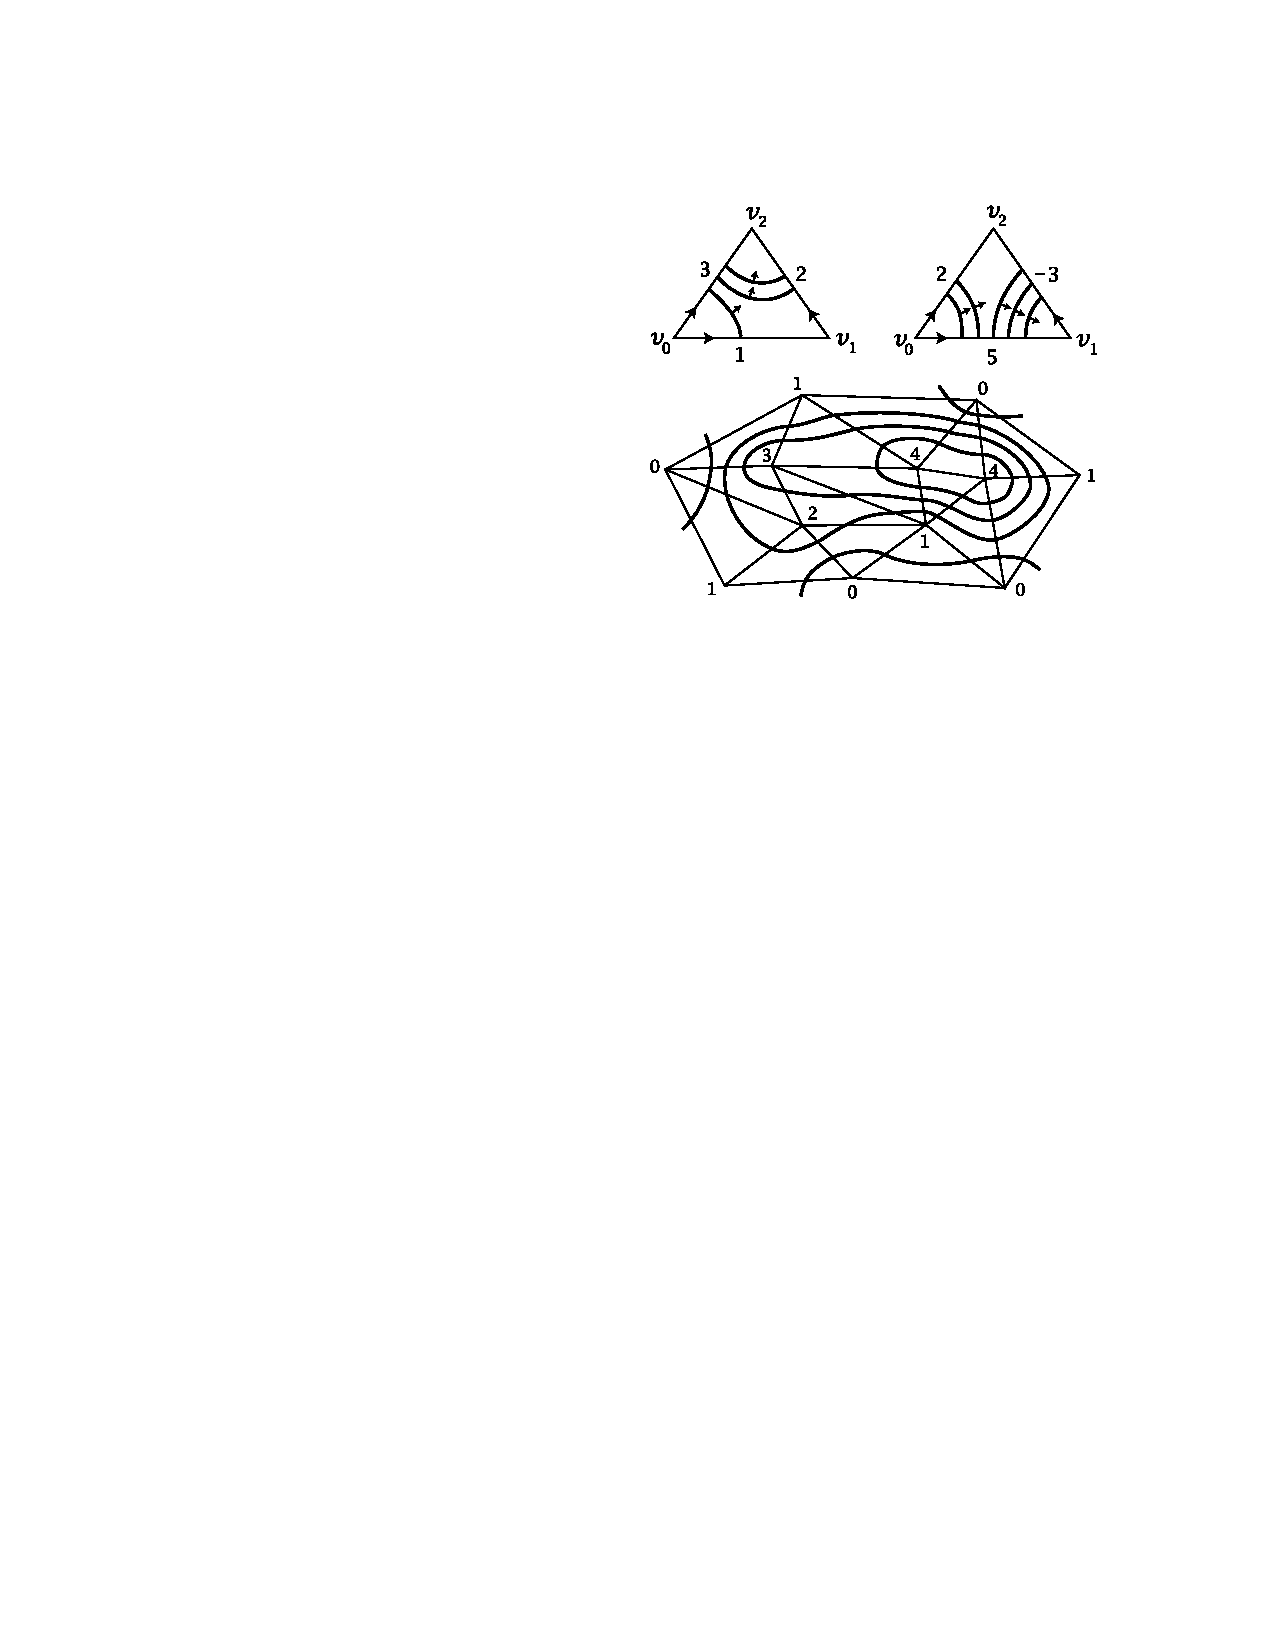
\includegraphics{idea-cohomo}\]
The resulting collection $C_\psi$ of disjoint curves in $X$ can be thought of as something like level curves for a function $\varphi$ with $\delta\varphi=\psi$, if such a function exists. The value of $\varphi$ changes by $1$ each time a curve of $C_\psi$ is crossed.
\end{itemize}
The key to relating cohomology groups to homology groups is the observation
that a function from $i$-simplices of $X$ to $G$ is equivalent to a homomorphismfromthe simplicial chain group $\Delta^i(X)$ to $G$. This is because $\Delta^i(X)$ is free abelian with basis the $i$-simplices of $X$, and a homomorphism with domain a free abelian group is uniquely determined by its values on basis elements, which can be assigned arbitrarily. Thus we have an identification of $\Delta^i(X;G)$ with the group $\Hom(\Delta_i(X),G)$ of homomorphisms $\Delta_i(X)\to G$, which is called the \textbf{dual group} of $\Delta_i(X)$. There is also a simple relationship of duality between the homomorphism $\delta:\Delta^i(X;G)\to\Delta^{i+1}(X;G)$ and the boundary
homomorphism $\partial:\Delta_{i+1}(X)\to\Delta_i(X)$. The general formula for $\delta$ is
\[\delta\varphi([v_0,\cdots,v_{i+1}])=\sum_{i}(-1)^j\varphi([v_0,\cdots,\widehat{v}_j,\cdots,v_{i+1}]).\]
and the latter sumis just $\varphi(\partial[v_0,\cdots,v_{i+1}])$. Thus we have $\delta\varphi=\varphi\partial$. In other words, $\delta$ sends each $\varphi\in\Hom(\Delta_i(X),G)$ to the composition 
\[\begin{tikzcd}
\Delta_{i+1}(X)\ar[r,"\partial"]&\Delta_i(X)\ar[r,"\varphi"]&G
\end{tikzcd}\]
which in the language of linear algebra means that $\delta$ is the \textbf{dual map} of $\partial$.\par
Thus we have the algebraic problem of understanding the relationship between
the homology groups of a chain complex and the homology groups of the dual complex obtained by applying the functor $C\mapsto\Hom(C,G)$. This is the first topic of the chapter.
\section{Cohomology Groups}
\subsection{Definition}
we observed that for any fixed abelian group $G$, there is a contravariant functor from the category of abelian groups to itself that sends each group $X$ to the group $\Hom(X,G)$ of homomorphisms into $G$, and each homomorphism $f:X\to Y$ to the induced homomorphism $f^*:\Hom(Y,G)\to\hom(X,G)$ given
by $f^*(\varphi)=\varphi\circ f$. We apply this to the singular chain groups as follows. Given a topological space $X$ and an abelian group $G$, for any integer $p\geq0$ let $C^p(X;G)$ denote the group $\Hom(C_p(X),G)$. Elements of $C^p(X;G)$ are called \textbf{$\bm{p}$-dimensional singular cochains with coefficients in $\bm{G}$} ($p$-cochains for short).\par
The boundary operator $\partial:C_{p+1}(X)\to C_p(X)$ induces a group homomorphism $\delta:C^p(X;G)\to C_{p+1}(X;G)$, called the coboundary operator, characterized by
\[(\delta\varphi)(c)=\varphi(\partial c).\]
It is immediate that $\delta^2=0$, so we have a chain complex
\[\begin{tikzcd}
\cdots\ar[r]&C^{p-1}(X;G)\ar[r,"\delta"]&C^{p}(X;G)\ar[r,"\delta"]&C^{p+1}(X;G)\ar[r,"\delta"]&\cdots
\end{tikzcd}\]
(Actually, when the arrows go in the direction of increasing indices as in this case, it is customary to call it a \textbf{cochain complex}.) A $p$-cochain $\varphi$ is called a \textbf{cocycle} if $\delta\varphi=0$, and a \textbf{coboundary} if there exists $\psi\in C^{p-1}(X;G)$ such that $\delta\psi=\varphi$. The subgroups of $C^p(X;G)$ consisting of cocycles and coboundaries are denoted by $Z^p(X;G)$ and $B^p(X;G)$, respectively.\par
We define the $p$-th singular cohomology group of $X$ with coefficients in $G$ to be the quotient
\[H^p(X;G):=\dfrac{Z^p(X;G)}{B^p(X;G)}.\]
If $f:X\to Y$ is a continuous map, we obtain a map $f^\sharp:C^p(Y;G)\to C^p(X;G)$ (note the reversal of direction) by 
\[(f^\flat\varphi)(c)=\varphi(f_\sharp c).\]
This map commutes with the coboundary operators because
\[(f^\flat\delta\varphi)(c)=\varphi(\partial f_\sharp c)=(f_\sharp\partial c)=(\delta f^\flat)(c).\]
(A map that commutes with $\delta$ is called, predictably enough, a \textbf{cochain map}.) Therefore,
$f^\flat$ induces a cohomology homomorphism $f^*:H^p(Y)\to H^p(X)$ by $f^*[\varphi]=[f^\flat\varphi]$.
\begin{proposition}[\textbf{Functorial Properties of Cohomology}]
The induced cohomology homomorphism satisfies the following properties.
\begin{itemize}
\item[$(a)$]If $f:X\to Y$ and $g:\to Z$ are continuous, then $(g\circ f)^*=g^*\circ f^*$.
\item[$(b)$]The homomorphism induced by the identity map is the identity.
\end{itemize}
Therefore, the assignments $X\mapsto H^p(X;G)$, $f\mapsto f^*$ define a contravariant functor from the category of topological spaces to the category of abelian groups.
\end{proposition}
\begin{corollary}
If $f:X\to Y$ is a homeomorphism, then for every abelian group $G$ and every integer $p\geq0$, the map
$f^*:H^p(Y;G)\to H^p(X;G)$ is an isomorphism.
\end{corollary}
In a very specific sense, the singular cohomology groups express the same information as the homology groups, but in rearranged form. The precise statement is given by the \textbf{universal coefficient theorem}, which gives an exact sequence from which the cohomology groups with any coefficients can be computed from the
singular homology groups.\par
We do not go into the general case here, but we can easily handle one special case. Let $\F$ be a field of characteristic zero (which just means that $\F$ is torsion-free as an abelian group under addition). In most applications $\F$ will be $\R$, $\C$, or $\Q$.We can form the cohomology groups $H^p(X;\F)$ as usual, just by regarding $\F$ as an abelian group; but in this case they have a bit more structure. The basic algebraic facts are expressed in the following lemma.
\begin{lemma}\label{Hom lem}
Let $\F$ be a field of characteristic zero.
\begin{itemize}
\item[$(a)$]For any abelian group $G$, the set $\Hom(G;\F)$ of group homomorphisms from $G$ to $\F$ is a vector space over $\F$ with scalar multiplication defined pointwise: $(a\varphi)(g)=a(\varphi(g))$ for $a\in\F$.
\item[$(b)$]If $f:G_1\to G_2$ is a group homomorphism, then the induced homomorphism $f^*:\Hom(G_2,\F)\to\Hom(G_1,\F)$ is an $\F$-linear map.
\item[$(c)$]If $G$ is finitely generated, the dimension of $\Hom(G,\F)$ is equal to the rank of $G$.
\end{itemize}
\end{lemma}
\begin{proof}
For $(c)$, we proceed as follows. First suppose $G$ is free abelian of rank $n$, and let $g_1,\cdots,g_n$ be a basis for $G$ (as an abelian group). For each $i$, define a homomorphism $\varphi_i:G\to\F$ by setting
\[\varphi_i(g_j)=\delta_{ij}.\]
If $\sum_ia_i\varphi_i$ is the zero homomorphism for some scalars $a_i\in\F$, applying this homomorphism to $g_j$ shows that $a_j=0$, so the $\varphi_i$'s are linearly independent. On the other hand, it is easy to see that an arbitrary $\varphi\in\Hom(G,\F)$ can be written $\sum_ia_i\varphi_i$ with $a_i=\varphi(g_i)$; thus the $\varphi_i$'s are a basis for $\Hom(G,\F)$, proving the result in this case.\par
In the general case, let $T\sub G$ be the torsion subgroup of $G$. The surjective homomorphism $\pi:G\to G/T$ induces a homomorphism
\[\pi^*:\Hom(G/T,\F)\to\Hom(G,\F).\]
It follows easily from the surjectivity of $\pi$ that $\pi^*$ is injective ($\Hom(-,M)$ is left exact for any $\Z$ module $M$). On the other hand, let $\varphi\in\Hom(G)$ be arbitrary. If $g\in G$ satisfies $kg=0$, then $\varphi(g)=\varphi(kg)/k=0$, so $T\sub\ker\varphi$ and $\varphi$ descends to a homomorphism $\widetilde{\varphi}\in\Hom(G/T,\F)$. Clearly, $\pi^*\widetilde{\varphi}=\varphi$, so $\pi^*$ is an isomorphism. Because $G/T$ is free abelian, we have $\dim\Hom(G,\F)=\dim\Hom(G/T,\F)=\rank G/T=\rank G$.
\end{proof}
Applying this to $C^p(X;\F)=\Hom(C_p(X),\F)$, we see that the cochain groups are $\F$-vector spaces and the coboundary operators are linear maps. It follows that $Z^p(X;\F)$ and $B^p(X;\F)$ are vector spaces as is the quotient $H^p(X;\F)$. Moreover, for any continuous map $f:X\to Y$, the induced cohomology map $f^*:H^p(X;\F)\to H^p(X;\F)$ is also a linear map.
The special feature of field coefficients that makes the cohomology groups easier to calculate is expressed in the following lemma.
\begin{lemma}[\textbf{Extension Lemma for Fields}]
Let $\F$ be a field of characteristic zero. If $G$ is an abelian group, any group homomorphism from a subgroup of $G$ to $\F$ admits an extension to all of $G$.
\end{lemma}
\begin{proof}
$\Z$ is a PID, any field is a $\Z$ module. Since $\F$ has characteristic zero, it is divisible, it is injective. So for any subgroup of $G$, we have
\[\begin{tikzcd}
0\ar[r]&H\ar[d]\ar[r]&G\ar[ld,dashed]\\
&\F
\end{tikzcd}\]
Thus the claim follows.
\end{proof}
\begin{theorem}
Let $\F$ be a field of characteristic zero. For any topological space $X$, the vector spaces $H^p(X;\F)$ and $\Hom(H_p(X),\F)$ are naturally isomorphic under
the map that sends $[\varphi]\in H^p(X;\F)$ to the homomorphism defined by $[c]\mapsto\varphi(c)$. Hence if $H_p(X)$ is finitely generated, then the dimension of $H^p(X;\F)$ is equal to the rank of $H_p(X)$.
\end{theorem}
\begin{proof}
The functor $\Hom(-,\F)$ is exact since $\F$ is injective, so the first claim follows. The second follows from Lemma~\ref{Hom lem}.
\end{proof}
As a consequence of this theorem, the Euler characteristic of a space can also be computed in terms of its cohomology. The following corollary follows immediately from the theorem.
\begin{corollary}
If $X$ is a topological space such that $H_p(X)$ is finitely generated for all $p$ and zero for $p$ sufficiently large, then for any field $\F$ of characteristic zero,
\[\chi(X)=\sum_p(-1)^p\dim H^p(X;\F).\]
\end{corollary}
\subsection{The Universal Coefficient Theorem}
Let's begin with a special case about $\RP^3$: Consider the chain complex
\[\begin{tikzcd}
0\ar[r]&\Z\ar[r,"0"]&\Z\ar[r,"2"]&\Z\ar[r,"0"]&\Z\ar[r]&0
\end{tikzcd}\]
If we dualize by taking $\Hom(-,G)$ with $G=\Z$, we obtain the cochain complex
\[\begin{tikzcd}
0&\Z\ar[l]&\Z\ar[l,swap,"0"]&\Z\ar[l,swap,"2"]&\Z\ar[l,swap,"0"]&0\ar[l]
\end{tikzcd}\]
In the original chain complex the homology groups are $\Z$'s in dimensions $0$ and $3$, together with a $\Z/2\Z$ in dimension $1$. The cohomology groups are again $\Z$'s in dimensions $0$ and $3$, but the $\Z/2\Z$ in the $1$-dimensional homology of the original complex has shifted up a dimension to become a $\Z/2\Z$ in $2$-dimensional cohomology.\par
Now our goal is to find some relations between the cohomology group $H^n(X)$ and the homology group $H_n(X)$. As we see above, this is just figuring out the effect of the functor $\Hom(-,G)$ on the homology of the complex. As one may guess, this should be related to the dereived functor $\Ext$, which turned out to be the truth. \textbf{To simplify the discussion, we will use some facts in Homological Algebra: such as $\bm{\Hom(-,G)}$ is left-exact, $\bm{\Ext^1(P,-)=0}$ for free abelian groups $\bm{P}$, ect.}\par
First consider a complex $C$:
\[\begin{tikzcd}
\cdots\ar[r]&C_{n+1}\ar[r,"\partial_{n+1}"]&C_n\ar[r,"\partial_{n}"]&C_{n-1}\ar[r]&\cdots
\end{tikzcd}\]
We can break it into short exact sequences:
\[\begin{tikzcd}
0\ar[r]&Z_n\ar[r]&C_n\ar[r]&B_{n-1}\ar[r]&0
\end{tikzcd}\]
And to apply the long exact seqeunce, we add zeros on the both sides to yield complexes
\[\begin{tikzcd}
&\vdots\ar[d]&\vdots\ar[d]&\vdots\ar[d]&\\
0\ar[r]&Z_{n+1}\ar[d,"0"]\ar[r]&C_{n+1}\ar[d,"\partial"]\ar[r,"\partial"]&B_{n}\ar[r]\ar[d,"0"]&0\\
0\ar[r]&Z_{n}\ar[r]\ar[d]&C_n\ar[r,"\partial"]\ar[d]&B_{n-1}\ar[r]\ar[d]&0\\
&\vdots&\vdots&\vdots&
\end{tikzcd}\]
and this gives a short exact sequence of chain complexes. Now we apply the functor $\Hom(-,G)$ to get
\[\begin{tikzcd}
&\vdots&\vdots&\vdots&\\
0&Z^*_{n+1}\ar[u]\ar[l]&C^*_{n+1}\ar[u]\ar[l]&B^*_{n}\ar[u]\ar[l,swap,"\delta"]&0\ar[l]\\
0&Z^*_{n}\ar[u,"0"]\ar[l]&C^*_n\ar[l]\ar[u,"\delta"]&B^*_{n-1}\ar[l,swap,"\delta"]\ar[u,"0"]&0\ar[l]\\
&\vdots\ar[u]&\vdots\ar[u]&\vdots\ar[u]&
\end{tikzcd}\]
Since $B_n$ are free abelian groups for each $n$, we conclude that the rows are still exact. So this is a short exact sequence of chain complexes, from which we get a long exact sequence
\[\begin{tikzcd}
\cdots&B_n^*\ar[l]&Z^*_{n}\ar[l]&H^n(C,G)\ar[l]&B_{n-1}^*\ar[l]&Z^*_{n-1}\ar[l]&\cdots\ar[l]
\end{tikzcd}\]
The connecting morphisms $Z^*_{n-1}\to B^*_{n-1}$ in thie sequence are the dual $i^*_n$ of the inclusions $i_n:B_n\hookrightarrow Z_n$: Recall how this morphism is constructed, we extend $\varphi\in Z^*_n$ to $C^*_n$, compose with $\delta$, and take preimage of $\delta$:
\[\begin{tikzcd}
&\widetilde{\varphi}\circ\partial&\widetilde{\varphi}\circ\partial\circ\partial^{-1}\ar[l,swap,"\delta"]\\
\varphi&\widetilde{\varphi}\ar[l]\ar[u,swap,"\delta"]&
\end{tikzcd}\]
The restrction $\varphi|_{B_n}$ is exactly the image. So we get the conclusion.\par
With this in mind, we begin to compute $H^n(C;G)$. First, from the long exact sequence we extract
\begin{equation}
\begin{tikzcd}
0&\ker i_n^*\ar[l]&H^n(C;G)\ar[l]&\coker i^*_{n-1}\ar[l]&0\ar[l]
\end{tikzcd}
\tag{$\ast$}
\end{equation}
What are kernels and coernels of these $i^*_n$? We consult the exact sequence:
\[\begin{tikzcd}
0\ar[r]&B_{n}\ar[r]&Z_n\ar[r]&H_n(C)\ar[r]&0
\end{tikzcd}\]
Applying $\Hom(-,G)$ gives a long exact sequence, in terms of the derived functor $\Ext^i(-,G)$:
\[\begin{tikzcd}
0&\Ext^1(H_n(C),G)\ar[l]&B^*_n\ar[l]&Z^*_n\ar[l,swap,"i^*_n"]&\Hom(H_n(C),G)\ar[l]&0\ar[l]
\end{tikzcd}\]
The leftmost term is $\Ext^1(Z_n,G)$, which is zero since $Z_n$ is free. Now with this we claim 
\[\ker i^*_n=\Hom(H_n(C),G),\quad \coker i^*_n=\Ext^1(H_n(C),G).\]
Plug into $(\ast)$ we get
\[\begin{tikzcd}
0&\Hom(H_{n}(C),G)\ar[l]&H^n(C;G)\ar[l]&\Ext^1(H_{n-1}(C),G)\ar[l]&0\ar[l]
\end{tikzcd}\]
Summarizing, we have established the following algebraic result:
\begin{theorem}[\textbf{universal coefficient theorem for cohomology}]\label{Universal coeff}
If a chain complex $C$ of free abelian groups has homology groups $H_n(C)$, then the cohomology groups $H_n(C;G)$ of the cochain complex $\Hom(C_n,G)$ are determined by split exact sequences
\[\begin{tikzcd}
0\ar[r]&\Ext^1(H_{n-1}(C),G)\ar[r]&H^n(C;G)\ar[r,"h"]&\Hom(H_{n}(C),G)\ar[r]&0
\end{tikzcd}\]
\end{theorem}
It is sometimes useful to describe what the morphism $h:H^n(C;G)\to\Hom(H_n(C),G)$ looks like: A class in $H^n(C;G)$ is
represented by a homomorphism $\varphi:C_n\to G$ such that $\delta\varphi=0$, that is, $\varphi\partial=0$, or in other words, $\varphi$ vanishes on $B_n$. The restriction $\varphi_0=\varphi|Z_n$ then induces a quotient homomorphism $\widetilde{\varphi}_0:Z_n/B_n\to G$, an element of $\Hom(H_n(C),G)$. If $\varphi$ is in $\im\delta$, say $\varphi=\delta\psi=\psi\partial$, then $\varphi$ is zero on $Z_n$, so $\varphi_0=0$ and hence also $\widetilde{\varphi}_0=0$, which means this map is well-defined. This is the homomorphism in the exact sequence. Conversely, for $\psi\in\Hom(H_n(C),G)$, we can extend it to $\Hom(C_n,G)$ by defining 
\[\psi(a):=\psi([a]).\]
Then $\varphi(a)=0$ for $a\in B_n$, hence $\delta\varphi=0$, making it an element in $H^n(C,G)$. The argument gives us a homomorphism $g:\Hom(H_n(C),G)\to H^n(C;G)$, which can be verified to be a right inverse of $h$. So the exact sequence in Theorem~\ref{Universal coeff} indeed splits.\par
Computing $\Ext^1(H,G)$ for finitely generated $H$ is not difficult using the following three properties:
\begin{itemize}
\item $\Ext(H\oplus H',G)=\Ext^1(H,G)\oplus\Ext^1(H',G)$.
\item $\Ext(H,G)=0$ if $H$ is free.
\item $\Ext(Z/n\Z,G)=G/nG$.
\end{itemize}
For the last equality, consider the following exact sequence
\[\begin{tikzcd}
0\ar[r]&\Z\ar[r,"\cdot n"]&\Z\ar[r]&\Z/n\Z\ar[r]&0
\end{tikzcd}\]
Applying $\Hom(-,G)$ gives
\[\begin{tikzcd}
0\ar[r]&\Z/n\Z^*\ar[r,"\cdot n"]&\Z^*\ar[r]&\Z^*\ar[r]&\Ext^1(\Z/n\Z,G)\ar[r]&0
\end{tikzcd}\]
Since $\Z^*=\Hom(\Z,G)\cong G$, and the map $\cdot n$ is defined to be 
\[n(\varphi)(x)=\varphi(nx)=n\varphi(x).\]
we conclude the image of $\cdot n$ is $nG$, so $\Ext^1(\Z/n\Z,G)=G/nG$.\par
In particular, these three properties imply that $\Ext^1(H,\Z)$ is isomorphic to the torsion subgroup of $H$ if $H$ is finitely generated. Further, observe that $\Hom(H,\Z)$ is isomorphic to the free part of $H$ if $H$ is finitely generated: Let $T\sub H$ be the torsion group, then for $x\in T$ and $\varphi\in\Hom(H,\Z)$ we have
\[n\varphi(x)=\varphi(nx)=\varphi(0)=0\text{ for $n$ such that $nx=0$}\]
This means every $\varphi$ vanishes on $T$, hence restricts to a morphism in $\Hom(H/T,\Z)$. So we have
\[\Hom(H,\Z)=\Hom(H/T,\Z)\cong H/T\]
since $H/T$ is free, and we use the fact $\Hom(\bigoplus_iM_i,\Z)=\prod_i\Hom(M_i,\Z)$.
\begin{corollary}
If the homology groups $H_n$ and $H_{n-1}$ of a chain complex $C$ of free abelian groups are finitely generated, with torsion subgroups $T_n\sub H_n$ and
$T_{n-1}\sub H_{n-1}$, then 
\[H^n(C;\Z)=(H_n/T_n)\oplus T_{n-1}\].
\end{corollary}
It is useful in many situations to know that the short exact sequences in the
universal coefficient theorem are natural, meaning that a chain map $\alpha$ between chain complexes $C$ and $C'$ of free abelian groups induces a commutative diagram
\[\begin{tikzcd}
0\ar[r]&\Ext^1(H_{n-1}(C),G)\ar[r]&H^n(C;G)\ar[r]&\Hom(H_{n}(C),G)\ar[r]&0\\
\
0\ar[r]&\Ext^1(H_{n-1}(C'),G)\ar[u,"(\alpha_*)^*"]\ar[r]&H^n(C';G)\ar[r]\ar[u,"\alpha^*"]&\Hom(H_{n}(C'),G)\ar[r]\ar[u,"(\alpha_*)^*"]&0
\end{tikzcd}\]
The naturality property together with the five-lemma proves:
\begin{corollary}\label{iso homo cohomo}
If a chain map between chain complexes of free abelian groups induces an isomorphism on homology groups, then it induces an isomorphism on cohomology
groups with any coefficient group $G$.
\end{corollary}
For the remainder of this section we will go through the main features of singular homology and check that they extend without much difficulty to cohomology.\par
\textbf{Reduced Groups}. Reduced cohomology groups $\widetilde{H}^n(X;G)$ can be defined by dualizing the augmented chain complex 
\[\begin{tikzcd}
\cdots\ar[r]&C_0(X)\ar[r,"\eps"]&\Z\ar[r]&0
\end{tikzcd}\]
then taking $\ker/\im$. As with homology, this gives $\widetilde{H}^n(X;G)=H^n(X;G)$ for $n>0$, and the universal coefficient theorem identifies $\widetilde{H}^0(X;G)$ with $\Hom(\widetilde{H}_0(X),G)$. We can describe the difference between $\widetilde{H}^0(X;G)$ and $H^0(X;G)$ more explicitly by using the interpretation of $H^0(X;G)$ as functions $X\to G$ that are constant on path-components. Recall that the augmentation map $\eps:C_0(X)\to\Z$ sends each singular $0$ simplex $\sigma$ to $1$, so the dual map $\eps^*$ sends a homomorphism $\varphi:\Z\to G$ to the composition
\[\begin{tikzcd}
C_0(X)\ar[r,"\eps"]&\Z\ar[r,"\varphi"]&G
\end{tikzcd}\]
which is the function $\sigma\mapsto\varphi(1)$. This is a constant function $X\to G$, and since $\varphi(1)$ can be any element of $G$, the image of $\eps^*$ consists of precisely the constant functions. Thus $\widetilde{H}^0(X;G)$ is all functions $X\to G$ that are constant on path-components modulo the functions that are constant on all of $X$.\par
\textbf{Relative Groups and the Long Exact Sequence of a Pair}. To define relative groups $H^n(X,A;G)$ for a pair $(X,A)$ we first dualize the short exact sequence
\[\begin{tikzcd}
0\ar[r]&C_n(A)\ar[r,"i"]&C_n(X)\ar[r,"j"]&C_n(X,A)\ar[r]&0
\end{tikzcd}\]
by applying $\Hom(-,G)$ to get 
\[\begin{tikzcd}
0&C^n(A)\ar[l]&C^n(X)\ar[l,swap,"i^*"]&C^n(X,A)\ar[l,swap,"j^*"]&0\ar[l]
\end{tikzcd}\]
where by definition $C_n(X,A;G)=\Hom(C_n(X,A),G)$. This sequence is exact by the
following direct argument. The map $i^*$ restricts a cochain on $X$ to a cochain on $A$. Thus for a function from singular $n$-simplices in $X$ to $G$, the image of this function under $i^*$ is obtained by restricting the domain of the function to singular $n$-simplices in $A$. Every function from singular $n$-simplices in $A$ to $G$ can be extended to be defined on all singular $n$-simplices in $X$, for example by assigning the value $0$ to all singular $n$-simplices not in $A$, so $i^*$ is surjective. The kernel of $i^*$ consists of cochains taking the value $0$ on singular $n$-simplices in $A$. Such cochains are the same as homomorphisms $C_n(X,A)=C_n(X)/C_n(A)\to G$, so the kernel of $i^*$ is exactly $C_n(X,A;G)=\Hom(C_n(X,A),G)$, giving the desired exactness. Notice that we can view $C_n(X,A;G)$ as the functions from singular $n$-simplices in $X$ to $G$ that vanish on simplices in $A$, since the basis for $C_n(X)$ consisting of singular $n$-simplices in $X$ is the disjoint union of the simplices with image contained in $A$ and the simplices with image not contained in $A$.\par
Relative coboundarymaps $\delta:C_n(X,A;G)\to C_{n+1}(X,A;G)$ are obtained as restrictions of the absolute $\delta$'s, so relative cohomology groups $H^n(X,A;G)$ are defined. The fact that the relative cochain group is a subgroup of the absolute cochains, namely the cochains vanishing on chains in $A$, means that relative cohomology is conceptually a little simpler than relative homology The maps $i^*$ and $j^*$ commute with $\delta$ since $i$ and $j$ commute with $\partial$, so the preceding displayed short exact sequence of cochain groups is part of a short exact sequence of cochain complexes, giving rise to an associated long exact sequence of cohomology groups
\[\begin{tikzcd}
\cdots\ar[r]&H^n(X,A;G)\ar[r]&H^{n+1}(A;G)\ar[r]&H^{n+1}(X;G)\ar[r]&H^{n+1}(X,A;G)\ar[r]&\cdots
\end{tikzcd}\]
By similar reasoning one obtains a long exact sequence of reduced cohomology groups for a pair $(X,A)$ with $A$ nonempty, where $\widetilde{H}^n(X,A;G)=H^n(X,A;G)$ for all $n$, as in homology. Taking $A$ to be a point $x_0$, this exact sequence gives an identification of $\widetilde{H}^n(X;G)$ with $H^n(X,x_0;G)$.\par
More generally there is a long exact sequence for a triple $(X,A,B)$ coming from
the short exact sequences
\[\begin{tikzcd}
0&C^n(A,B;G)\ar[l]&C^n(X,B;G)\ar[l,swap,"i^*"]&C^n(X,A;G)\ar[l,swap,"j^*"]&0\ar[l]
\end{tikzcd}\]
The long exact sequence of reduced cohomology can be regarded as the special case that $B$ is a point.\par
As one would expect, there is a duality relationship between the connecting homomorphisms $\delta:H^n(A;G)\to H^n(X,A;G)$ and $\partial:H_n(X,A)\to H_n(A)$. This takes the form of the following commutative diagram
\[\begin{tikzcd}
H^n(A;G)\ar[r,"\delta"]\ar[d,"h"]&H^n(X,A;G)\ar[d,"h"]\\
\Hom(H_n(A),G)\ar[r,"\partial^*"]&\Hom(H_n(X,A),G)
\end{tikzcd}\]
To verify commutativity, recall how the two connecting homomorphisms are defined, via the diagrams
\[\begin{tikzcd}
&C^{n+1}(X;G)&C^{n+1}(X,A;G)\ar[l]\\
C^n(A;G)\ar[rru,dashed]&C^n(X;G)\ar[l]\ar[u]
\end{tikzcd}\quad\quad\begin{tikzcd}
&C_{n+1}(X)\ar[r]\ar[d]&C_{n+1}(X,A)\ar[lld,dashed]\\
C_n(A)\ar[r]&C_n(X)&
\end{tikzcd}\]
The connecting homomorphisms are represented by the dashed arrows, which are well-defined only when the chain and cochain groups are replaced by homology and
cohomology groups. To show that $h\delta=\partial^*h$, start with an element $\alpha\in H^n(A;G)$ represented by a cocycle $\varphi\in C^n(A;G)$. To compute $\delta(\alpha)$ we first extend $\varphi$ to a cochain $\widetilde{\varphi}\in C^n(X;G)$, say by letting it take the value $0$ on singular simplices not in
$A$. Then we compose $\widetilde{\varphi}$ with $\partial:C_{n+1}(X)\to C_n(X)$ to get a cochain $\widetilde{\varphi}\partial\in C^{n+1}(X;G)$, which actually lies in $C^{n+1}(X,A;G)$ since the original $\varphi$ was a cocycle in $C^n(A;G)$. This cochain $\widetilde{\varphi}\partial\in C^{n+1}(X,A;G)$ represents $\delta(\alpha)$ in $H^{n+1}(X,A;G)$. Now we apply the map $h$, which simply restricts the domain of $\widetilde{\varphi}\partial$ to relative cycles in $C^{n+1}(X,A)$, that is, $(n+1)$-chains in $X$ whose boundary lies in $A$. On such chains we have $\widetilde{\varphi}\partial=\varphi\partial$ since the extension of $\varphi$ to $\widetilde{\varphi}$ is irrelevant. The net result of all this is that $h\delta(\alpha)$ is represented by $\varphi\partial$. Let us compare this with $\partial^*h(\alpha)$. Applying $h$ to $\varphi$ restricts its domain to cycles in $A$. Then applying $\partial^*$ composes with the map which sends a relative $(n+1)$ cycle in $X$ to its boundary in $A$. Thus $\partial^*h(\alpha)$ is represented by $\varphi\partial$ just as $h\delta(\alpha)$ was, and so the square commutes.\par
\textbf{Induced Homomorphisms}. Dual to the chain maps $f_\sharp:C_n(X)\to C_n(Y)$ induced by $f:X\to Y$ are the cochain maps $f^\flat:C^n(Y;G)\to C^n(X;G)$. The relation $f_\sharp\partial=\partial f_\sharp$ dualizes to $\delta f^\flat=f^\flat\delta$, so $f^\flat$ induces homomorphisms $f^*:H^n(Y;G)\to H^n(X;G)$. In the relative case a map $f:(X,A)\to (Y,B)$ induces $f^*:H^n(Y, B;G)\to H^n(X,A;G)$ by the same reasoning, and in fact $f$ induces a map between short exact sequences of cochain complexes, hence amap between long exact sequences of cohomology groups, with commuting squares. The properties $(fg)^\flat=g^\flat f^\flat$ and $id^\flat=id$ imply $(fg)^*=g^*f^*$ and $id^*=id$, so $X\mapsto H_n(X;G)$ and $(X,A)\mapsto H^n(X,A;G)$ are contravariant functors, the \textit{contra} indicating that induced maps go in the reverse direction.\par
The algebraic universal coefficient theorem applies also to relative cohomology
since the relative chain groups $C^n(X,A)$ are free, and there is a naturality statement: A map $f:(X,A)\to(Y,B)$ induces a commutative diagram
\[\begin{tikzcd}
0\ar[r]&\Ext^1(H_{n-1}(X,A),G)\ar[r]&H^n(X,A;G)\ar[r,"h"]&\Hom(H_n(X,A),G)\ar[r]&0\\
0\ar[r]&\Ext^1(H_{n-1}(Y,B),G)\ar[u,"(f_*)^*"]\ar[r]&H^n(Y,B;G)\ar[u,"f^*"]\ar[r,"h"]&\Hom(H_n(Y,B),G)\ar[u,"(f_*)^*"]\ar[r]&0
\end{tikzcd}\]
This follows from the naturality of the algebraic universal coefficient sequences since the vertical maps are induced by the chain maps $f_\sharp:C_n(X,A)\to C_n(Y,B)$. When the subspaces $A$ and $B$ are empty we obtain the absolute forms of these results.\par
\textbf{Homotopy Invariance}. The statement is that if $f\simeq g:(X,A)\to (Y,B)$, then $f^*=g^*:H^n(Y,B)\to H^n(X,A)$. This is proved by direct dualization of the proof for homology. A chain homotopy $g_\sharp-f_\sharp=\partial h+h\partial$ dualizes to $g^\flat-f^\flat=h^*\delta+\delta h^*$.\par
\textbf{Excision}. For cohomology this says that for subspaces $Z\sub A\sub X$ with the closure of $Z$ contained in the interior of $A$, the inclusion $i:(X-Z,A-Z)֓\hookrightarrow(X,A)$ induces isomorphisms $i^*:H^n(X,A;G)\to H^n(X-Z,A-Z;G)$ for all $n$. This follows from the corresponding result for homology by the naturality of the universal coefficient theorem and the five-lemma.\par
\textbf{Simplicial Cohomology}. If X is a $\Delta$-complex and $A\sub X$ is a subcomplex, then the simplicial chain groups $\Delta_n(X,A)$ dualize to simplicial cochain groups $\Delta^n(X,A;G)=\Hom(\Delta_n(X,A),G)$, and the resulting cohomology groups are by definition the simplicial cohomology groups $H^n_\Delta(X,A;G)$. Since the inclusions $\Delta_n(X,A)\sub C_n(X,A)$ induce isomorphisms $H_n^\Delta(X,A)=H_n(X,A)$, Corollary~\ref{iso homo cohomo} gives the isomorphisms $H^n(X,A;G)=H^n_\Delta(X,A;G)$.\par
\textbf{Cellular Cohomology}. For a CW complex $X$ this is defined via the cellular cochain complex formed by the horizontal sequence in the following diagram, where coefficients in a given group $G$ are understood, and the cellular coboundary maps $d_n$ are the compositions $\delta_nj_n$, making the triangles commute. Note that $d_nd_{n-1}=0$ since
$j_n\delta_{n-1}=0$. 
\[\begin{tikzpicture}[scale=0.85]
\node (0) at (0,0) {$\cdots$};
\node (k0) at (4,0) {$H^{n-1}(X^{n-1},X^{n-2})$};
\node (k1) at (8,0) {$H^{n}(X^{n},X^{n-1})$};
\node (k2) at (12,0) {$H^{n+1}(X^{n+1},X^{n})$};
\node (k3) at (16,0) {$\cdots$};
\node (a1) at (6,1) {$H^{n-1}(X^{n-1})$};
\node (a2) at (8,2) {$0$};
\node (b1) at (10,-1) {$H^{n}(X^{n})$};
\node (b0) at (8,-2) {$H^n(X^{n+1})$};
\node (b2) at (12,-2) {$0$};
\node (b3) at (6,-3) {$0$};
\draw[->]
(0) edge (k0)
(k0) edge (k1)
(k2) edge (k3)
(a1) edge (a2)
(b1) edge (b2)
(b3) edge (b0)
(b0) edge (b1)
(k0) edge node[node font=\tiny,auto] {$d_{n-1}$} (k1)
(k1) edge node[node font=\tiny,auto] {$d_{n}$} (k2)
(k0) edge node[node font=\tiny,auto] {$j_{n-1}$} (a1) 
(a1) edge node[node font=\tiny,auto] {$\delta_{n-1}$} (k1)
(k1) edge node[node font=\tiny,below,pos=0.2] {$j_{n}$} (b1) 
(b1) edge node[node font=\tiny,below,pos=0.8,xshift=6pt] {$\delta_{n}$}(k2);
\end{tikzpicture}\]
\begin{theorem}
$H^n(X;G)=\ker d_n/\im d_{n-1}$. Furthermore, the cellular cochain complex is isomorphic to the dual of the cellular chain complex, obtained by applying $\Hom(-,G)$.
\end{theorem}
\begin{proof}
The universal coefficient theorem implies that $H^k(X^n,X^{n-1};G)=0$ for $k\neq n$. The long exact sequence of the pair $(X^n,X^{n-1})$ then gives isomorphisms $H^k(X^n;G)=H^k(X^{n-1};G)$ for $k\neq n,n-1$. Hence by induction on $n$ we obtain $H^k(X^n;G)=0$ if $k>n$. Thus the diagonal sequences in the preceding diagramare exact. The universal coefficient theorem also gives $H^k(X,X^{n+1};G)=0$ for $k\leq n+1$, so $H^n(X;G)=H^n(X^{n+1};G)$. The diagram then yields isomorphisms
\[H^n(X;G)=H^n(X^{n+1};G)=\ker\delta_n=\ker d_n/\ker j_{n}=\ker d_n/\im\delta_{n-1}=\ker d_n/\im d_{n-1}.\]
Where we use a lemma states that for $d=\delta\circ j$ and $j$ is surjective, we have
\[\ker\delta=\dfrac{\ker d}{\ker j},\]
by the induced surjective map $\ker d\stackrel{j}{\longrightarrow}\ker\delta$.\par
For the second statement in the theorem we have the diagram
\[\begin{tikzcd}
H^k(X^k,X^{k-1};G)\ar[r]\ar[d,"h"]&H^k(X^k;G)\ar[r,"\delta"]\ar[d,"h"]&H^{k+1}(X^{k+1},X^k;G)\ar[d,"h"]\\
\Hom(H_k(X^k,X^{k-1}),G)\ar[r]&\Hom(H_k(X^k),G)\ar[r,"\partial^*"]&\Hom(H_{k+1}(X^{k+1},X^k),G)
\end{tikzcd}\]
The cellular coboundary map is the composition across the top, and we want to see that this is the same as the composition across the bottom. The first and third vertical maps are isomorphisms by the universal coefficient theorem, so it suffices to show the diagram commutes. The first square commutes by naturality of $h$, and commutativity of the second square was shown in the discussion of the long exact sequence of cohomology groups of a pair $(X,A)$.
\end{proof}
\textbf{Mayer-Vietoris Sequences}. In the absolute case these take the form
\[\begin{tikzcd}
\cdots\ar[r]&H^n(X;G)\ar[r,"\Psi"]&H^n(A;G)\oplus H^n(B;G)\ar[r,"\Phi"]&H^n(A\cap B)\ar[r,"\delta"]&H^{n+1}(X;G)\ar[r]&\cdots
\end{tikzcd}\]
where $X$ is the union of the interiors of $A$ and $B$. This comes from the long exact sequence of the pairs $(B,A\cap B)$ and $(X,A)$, using Excision and Barratt-Whitehead Lemma.\par
There is also a relative Mayer-Vietoris sequence
\[\begin{tikzcd}
\cdots\ar[r]&H^n(X,Y;G)\ar[r,"\Psi"]&H^n(A,C;G)\oplus H^n(B,D;G)\ar[r,"\Phi"]&H^n(A\cap B,C\cap D)\ar[r]&\cdots
\end{tikzcd}\]
for a pair $(X,Y)=(A\cup B,C\cup D)$ with $C\sub A$ and $D\sub B$ such that $X$ is the union of the interiors of $A$ and $B$ while $Y$ is the union of the interiors of $C$ and $D$. To derive this, consider first the map of short exact sequences of cochain complexes
\[\begin{tikzcd}
0\ar[r]&C^n(X,Y;G)\ar[d]\ar[r]&C^n(X;G)\ar[r]\ar[d]&C^n(Y;G)\ar[d]\ar[r]&0\\
0\ar[r]&C^n(A+B,C+D;G)\ar[r]&C^n(A+B;G)\ar[r]&C^n(C+D;G)\ar[r]&0
\end{tikzcd}\]
Here $C^n(A+B,C+D;G)$ is defined as the kernel of $C^n(A+B;G)\to C^n(C+D;G)$, the restriction map, so the second sequence is exact. The vertical maps are restrictions. The second and third of these induce isomorphisms on cohomology, as we have seen, so by the five-lemma the first verticalmap also induces isomorphisms on cohomology. The relative Mayer-Vietoris sequence is then the long exact sequence associated to the short exact sequence of cochain complexes
\[\begin{tikzcd}[column sep=small]
0\ar[r]&C^n(A+B,C+D;G)\ar[r,"\psi"]&C^n(A,C;G)\oplus C^n(B,D;G)\ar[r,"\varphi"]&C^n(A\cap B,C\cap D;G)\ar[r]&0
\end{tikzcd}\]
This is exact since it is the dual of the short exact sequence
\[\begin{tikzcd}
0\ar[r]&C_n(A\cap B,C\cap D)\ar[r]&C_n(A,C)\oplus C_n(B,D)\ar[r]&C_n(A+B,C+D)\ar[r]&0
\end{tikzcd}\]
which splits since $C_n(A+B,C+D)$ is free with basis the singular $n$-simplices in $A$ or in $B$ that do not lie in $C$ or in $D$.
\subsection{Exercise}
\begin{exercise}
Show that the maps $G\stackrel{m}{\longrightarrow}G$ and $H\stackrel{n}{\longrightarrow}H$ multiplying each element by the integer $n$ induce multiplication by $n$ in $\Ext^1(H,G)$.
\end{exercise}
\begin{proof}
Let's de the case for $G\stackrel{m}{\longrightarrow}G$: Consider the diagram
\[\begin{tikzcd}
0\ar[r]&G\ar[r,"f_0"]\ar[d,"m"]&Q_0\ar[r]\ar[d,"\alpha_0"]&Q_1\ar[r]&\cdots\\
0\ar[r]&G\ar[r,"f_0"]&Q_0\ar[r]&Q_1\ar[r]&\cdots
\end{tikzcd}\]
The map $\alpha_0$ is induced by the composition $G\stackrel{m}{\longrightarrow}G\to Q_0$ and that $Q_0$ is injective. Since we have
\[\alpha_0\circ f_0(g)=f_0(mx)=mf_0(x)\]
$\alpha_0$ is multiplication by $m$.
\end{proof}
\begin{exercise}
Regarding $\Z/2\Z$ as a module over the ring $\Z/4\Z$, construct a resolution of $\Z/2\Z$ by free modules over $\Z/4\Z$ and use this to show that $\Ext^n_{\Z/4\Z}(\Z/2\Z,\Z/2\Z)$ is nonzero for all $n$.
\end{exercise}
\begin{proof}
The free resolution is infinite:
\[\begin{tikzcd}
\cdots\ar[r]&\Z/4\Z\ar[r,"\alpha_1"]&\Z/4\Z\ar[r,"\alpha_0"]&\Z/2\Z\ar[r]&0
\end{tikzcd}\]
where $\alpha_0:\Z/4\Z\to\Z/2\Z$ is the quotient map as follows
\[\alpha_0(0)=\alpha_0(2)=0,\quad \alpha(1)=\alpha(3)=1.\]
Hence $\ker\alpha_0=\{0,2\}$. Since this is isomorphic to $\Z/2\Z$, we construct $\alpha_i, i>0$ to be $\alpha_i=2\alpha_0$, that is, for $i>0$
\[\alpha_i(0)=\alpha_i(2)=0,\quad\alpha_i(1)=\alpha_i(3)=2.\]
And we get $\ker\alpha_i=\im\alpha_i=\{0,2\}$, so this complex is exact.\par
Applying $\Hom(-,\Z/2\Z)$ gives
\[\begin{tikzcd}
0\ar[r]&\Hom(\Z/2\Z,\Z/2\Z)\ar[r]&\Hom(\Z/4\Z,\Z/2\Z)\ar[r,"\alpha_1^*"]&\Hom(\Z/4\Z,\Z/2\Z)\ar[r]&\cdots
\end{tikzcd}\]
Every map $\varphi$ in the image of $\alpha_i$ is obtained by the following
\[\begin{tikzcd}
&\Z/4\Z&\\
\Z/4\Z\ar[ru,dashed]\ar[r,"\alpha_i"]&\{0,2\}\ar[r,hook]&\Z/4\Z\ar[lu]
\end{tikzcd}\]
Assume $\varphi=\alpha_i^*\psi=\psi\circ\alpha_i$, then $\varphi$ satisfies 
\[\varphi(0)=\varphi(2)=\psi(0)=0,\quad\varphi(1)=\varphi(3)=\psi(2).\]
But, note that for a map $\psi:\Z/4\Z\to\Z/2\Z$, we have $\psi(2)=2\psi(1)=0$. So the image of $\alpha^*$ is infact zero. So for all $n$ \[\Ext^n_{\Z/4\Z}(\Z/2\Z,\Z/2\Z)=\Hom_{\Z/4\Z}(\Z/4\Z,\Z/2\Z).\]
\end{proof}
\begin{exercise}
What happens if one defines homology groups $h_n(X;G)$ as the homology groups
of the chain complex 
\[\begin{tikzcd}
\cdots\ar[r]&\Hom(G,C_n(X))\ar[r]&\Hom(G,C_{n-1}(X))\ar[r]&\cdots
\end{tikzcd}\]
More specifically, what are the groups $h_n(X;G)$ when $G=\Z$, $\Z/m\Z$, and $\Q$?
\end{exercise}
\begin{proof}
$\Z$ are projective, so it produces nothing interesting. $\Hom(-,\Z)$ kills torsion, so $\Z/m\Z$ is not interesting either.\par
$\Q$ is divisible, so its quotient subgroups are all divisible. For $\varphi\in\Hom(\Q,\Z)$, the image $\im\varphi$ is a quotient subgroup of $\Q$. But there is no divisible subgroup of $\Z$ except $0$. So $\varphi$ is trivial. It follows that $\Hom(\Q,\Z)=0$. So if $C_n(X)$ is a finite sum, then $\Hom(\Q,C_n(X))=0$.
\end{proof}
\begin{exercise}
Regarding a cochain $\varphi\in C^1(X;G)$ as a function from paths in $X$ to $G$, show that if $\varphi$ is a cocycle, then
\begin{itemize}
\item[$(a)$]$\varphi(f\ast g)=\varphi(f)+\varphi(g)$.
\item[$(b)$]$\varphi$ takes the value $0$ on constant paths.
\item[$(c)$]$\varphi(f)=\varphi(g)$ if $f\simeq g$.
\item[$(d)$]$\varphi$ is a coboundary iff $\varphi(f)$ depends only on the endpoints of $f$, for all $f$.
\end{itemize}
In particular, $(a)$ and $(c)$ give a map $H^1(X;G)\to\Hom(\pi_1(X),G)$, which the universal coefficient theorem says is an isomorphism if $X$ is path-connected.
\end{exercise}
\begin{proof}
Since $\varphi$ is a cochain, it vanishes on boundaries, so it restricts to a map on $H_1(X)$:
\[\varphi([f]_H)=\varphi(f+\partial c)=\varphi(f).\]
\begin{itemize}
\item[$(a)$]By the Hurewicz homomorphism, $[f\ast g]_H=[f]_{H}+[g]_{H}$. So $\varphi(f\ast g)=\varphi([f\ast g]_H)=\varphi(f)+\varphi(g)$.
\item[$(b)$]Again from the Hurewicz homomorphism.
\item[$(c)$]If $f\ast g$, then $[f]=[g]$. Our claim follows.
\item[$(d)$]$\varphi$ is a coboundary iff $\varphi=\delta\psi=\psi\circ\partial$ for $\psi\in C^0(X;G)$. If this is satisfied, obviously we have $\varphi(f)=\psi(\partial f)$, so $\varphi(f)$ depends only on end points. Conversely, if $\varphi$ vanishes on loops, we can define a functoion $\psi\in C^0(X,G)$: choose a base point $x_0$, for any point $x\in X$, define $\psi(x)=\varphi(\alpha)$ for an arbitrary path $\alpha$ from $x_0$ to $x$. Then for a path $f\in C_1(X)$ we have
\[\delta\psi(f)=\psi(\partial f)=\psi(f(1)-f(0))=\varphi(\alpha_1)-\varphi(\alpha_0).\]
where $\alpha_1$, $\alpha_0$ are paths to $f(1)$, $f(0)$, respectively. Since $\alpha_0\ast f\ast\widebar{\alpha}_1$ is a loop at $x_0$, we have
\[\varphi(\alpha_0\ast f\ast\widebar{\alpha}_1)=\varphi(\alpha_0)+\varphi(f)-\varphi(\alpha_1).\]
This gives $\delta\psi(f)=\varphi(f)$. So $\varphi=\delta\psi$, showing that $\varphi$ is a coboundary.\par
Any way, this deals the case when $X$ has one component. For the case $X$ is not path-connected, we can do this in each component separately. Since the image of a path $f$ is contained in one component, we also get the claim.
\end{itemize}
\end{proof}
\begin{remark}
This gives the idea of De Rham cohomology: For a differential form $\omega$, the map
\[a\mapsto\int_{a}\omega\]
is a map from $C_n(X)$ to $\R$. So this is an element in $C^n(X,\R)$. For suitable spaces, the cohomology can be computed only use these differential forms. And on these forms, the differential $\delta$ becomes
\[\delta\int\omega=\int\omega\circ\partial=\int_{\partial}\omega\]
Recall the Stokes theorem, for a chain $a\in C_n(X)$ we have
\[\int_{\partial a}\omega=\int_a d\omega\]
where $d$ is the exterior differential. So we can directly define $\delta\omega=d\omega$, and this gives a cochain complex.
\end{remark}
\begin{exercise}
\mbox{}
\begin{itemize}
\item[$(a)$]Directly from the definitions, compute the simplicial cohomology groups of $S^1\times S^1$ with $\Z$ and $\Z/2\Z$ coefficients.
\item[$(a)$]Do the same for $\RP^2$ and the Klein bottle.
\end{itemize}
\end{exercise}
\begin{exercise}
Show that if $f:S^n\to S^n$ has degree $d$ then $f^*:H^n(S^n;G)\to H^n(S^n;G)$ is multiplication by $d$.
\end{exercise}
\begin{exercise}
Let $X$ be a Moore space $M(\Z/m\Z,n)$ obtained from $S^n$ by attaching a cell $e^{n+1}$ by a map of degree $m$.
\begin{itemize}
\item[$(a)$]Show that the quotient map $X\to X/S^n=S^{n+1}$ induces the trivial map on $\widetilde{H}_i(-;\Z)$ for all $i$, but not on $H^{n+1}(-;\Z)$. Deduce that the splitting in the universal coefficient
theorem for cohomology cannot be natural.
\item[$(b)$]Show that the inclusion $S^n֓\hookrightarrow X$ induces the trivial map on $\widetilde{H}^i(-;\Z)$ for all $i$, but not on $H^n(-;\Z)$.
\end{itemize}
\end{exercise}
\begin{proof}
\mbox{}
\begin{itemize}
\item[$(a)$]By universal coefficient theorem we obtain
\[\widetilde{H}_i(X,\Z)=\begin{cases}
\Z/m\Z&\text{if }i=n\\
0&\text{otherwise}
\end{cases}\quad \widetilde{H}_i(S^n,\Z)=\begin{cases}
\Z&\text{if }i=n\\
0&\text{otherwise}
\end{cases}\]
So the induced maps on homology are all zero. The cohomology is 
\[\widetilde{H}_i(X,\Z)=\begin{cases}
\Z/m\Z&\text{if }i=n+1\\
0&\text{otherwise}
\end{cases}\]
It is clear that the quotient induces identity on homology. But the induced map $H^{n+1}(S^n)\to H^{n+1}(X)$ is the quotient map $\Z\to\Z/m\Z$, which is not trivial. Now consider the following diagram
\[\begin{tikzcd}
0\ar[r]&\Ext^1(H_{n}(X),\Z)\ar[r]&H^{n+1}(X;\Z)\ar[r,shift left=0.5 ex,"h"]&\Hom(H_{n+1}(X),\Z)\ar[l,shift left=0.5ex,"g"]\ar[r]&0\\
\
0\ar[r]&\Ext^1(H_{n}(S^{n+1}),\Z)\ar[u,"(q_*)^*"]\ar[r]&H^{n+1}(S^{n+1};\Z)\ar[u,"q^*"]\ar[r,shift left=0.5 ex,"h"]&\Hom(H_{n+1}(S^{n+1}),\Z)\ar[u,"(q_*)^*"]\ar[l,shift left=0.5ex,"g"]\ar[r]&0
\end{tikzcd}\]
The right-hand side $(q_*)^*$ is zero since $\Hom(H_{n+1}(X),\Z)=0$. So the squre about $h$ commutes. But the squre about $g$ does not commute: one composition is zero, the other is the quotient $\Z\to\Z/m\Z$.
\item[$(b)$]Similar with $(a)$.
\end{itemize}
\end{proof}
\section{Cup Product}
To define the cup product we consider cohomology with coefficients in a ring $R$, the most common choices being $\Z$, $\Z/n\Z$, and $\Q$. For cochains $\varphi\in C^k(X;R)$ and $\psi\in C^\ell(X;R)$, the cup product $\varphi\cup\psi\in C^{k+\ell}(X;R)$ is the cochain whose value on a singular simplex $\sigma:\Delta^{k+\ell}\to X$ is given by the formula
\[(\varphi\cup\psi)(\sigma)=\varphi(\sigma|[v_0,\cdots,v_k])\,\psi(\sigma|[v_{k},\cdots,v_{k+\ell}])\]
where the right-hand side is the product in $R$. To see that this cup product of cochains induces a cup product of cohomology classes we need a formula relating it to the coboundary map:
\begin{lemma}
$\delta(\varphi\cup\psi)=\delta\varphi\cup\psi+(-1)^{k}\varphi\cup\delta\psi$ for $\varphi\in C^k(X;R)$ and $\psi\in C^\ell(X;R)$.
\end{lemma}
\begin{proof}
For $\sigma:\Delta^{k+\ell+1}\to X$ we have
\begin{align*}
\delta(\varphi\cup\psi)(\sigma)&=(\varphi\cup\psi)(\partial\sigma)=(\varphi\cup\psi)\Big(\sum_{i=0}^{k+\ell+1}(-1)^i\sigma|[v_0,\cdots,\widehat{v}_i,\cdots,v_{k+\ell+1}]\Big)\\
&=\sum_{i=0}^{k+\ell+1}(\varphi\cup\psi)(\sigma|[v_0,\cdots,\widehat{v}_i,\cdots,v_{k+\ell+1}])\\
&=\sum_{i=0}^{k+1}(-1)^i\varphi(\sigma|[v_0,\cdots,\widehat{v}_i,\cdots,v_{k+1}])\,\psi(\sigma|[v_{k+1},\cdots,v_{k+\ell+1}])\\
&+\sum_{i=k}^{k+\ell+1}(-1)^i\varphi(\sigma|[v_0,\cdots,v_k])\,\psi(\sigma|[v_{k},\cdots,\widehat{v}_i,\cdots,v_{k+\ell+1}])
\end{align*}
the last equation holds since the last term of the first sum cancels the first term of the second sum. Note that
\[(\delta\varphi\cup\psi)(\sigma)=\sum_{i=0}^{k+1}(-1)^i\varphi(\sigma|[v_0,\cdots,\widehat{v}_i,\cdots,v_{k+1}])\,\psi(\sigma|[v_{k+1},\cdots,v_{k+\ell+1}])\]
\[(-1)^k(\varphi\cup\delta\psi)(\sigma)=\sum_{i=k}^{k+\ell+1}(-1)^i\varphi(\sigma|[v_0,\cdots,v_k])\,\psi(\sigma|[v_{k},\cdots,\widehat{v}_i,\cdots,v_{k+\ell+1}])\]
so we get the formula.
\end{proof}
From the formula $\delta(\varphi\cup\psi)=\delta\varphi\cup\psi\pm\varphi\cup\delta\psi$ it is apparent that the cup product of two cocycles is again a cocycle. Also, the cup product of a cocycle and a coboundary, in either order, is a coboundary since $\varphi\cup\delta\psi=\pm\delta(\varphi\cup\psi)$ if $\delta\varphi=0$,
and $\delta\varphi\cup\psi=\delta(\varphi\cup\psi)$ if $\delta\psi=0$. It follows that there is an induced cup product
\[\begin{tikzcd}
H^k(X;R)\times H^\ell(X;R)\ar[r,"\cup"]&H^{k+\ell}(X;R)
\end{tikzcd}\]
This is associative and distributive since at the level of cochains the cup product obviously has these properties. If $R$ has an identity element, then there is an identity element for cup product, the class $1\in H^0(X;R)$ defined by the $0$ cocycle taking the value $1$ on each singular $0$-simplex.
A cup product for simplicial cohomology can be defined by the same formula as
for singular cohomology, so the canonical isomorphismbetween simplicial and singular cohomology respects cup products.
\begin{example}\label{cup prod eg}
Let $X$ be the $2$-dimensional CW complex obtained by attaching a $2$ cell
to $S^1$ by the degree $m$ map $S^1\to S^1, z\mapsto z^m$, so $X=M(\Z/m\Z,2)$ Using cellular cohomology, or cellular homology and the universal coefficient theorem, we see that $H^n(X;\Z)$ consists of a $\Z$ for $n=0$ and a $\Z/m\Z$ for $n=2$, so the cup product structure with $\Z$ coefficients is uninteresting. However, with $\Z/m\Z$ coefficients we have $H^i(X;\Z/m\Z)=\Z/m\Z$ for $i=0,1,2$, so there is the possibility that the cup product of two $1$-dimensional classes can be nontrivial.\par
To obtain a $\Delta$-complex structure on $X$, take a regular $m$-gon subdivided into $m$ triangles $T_i$ around a central vertex $v$, as shown in the figure for the case $m=4$, then identify all the outer edges by rotations of the $m$-gon. 
\[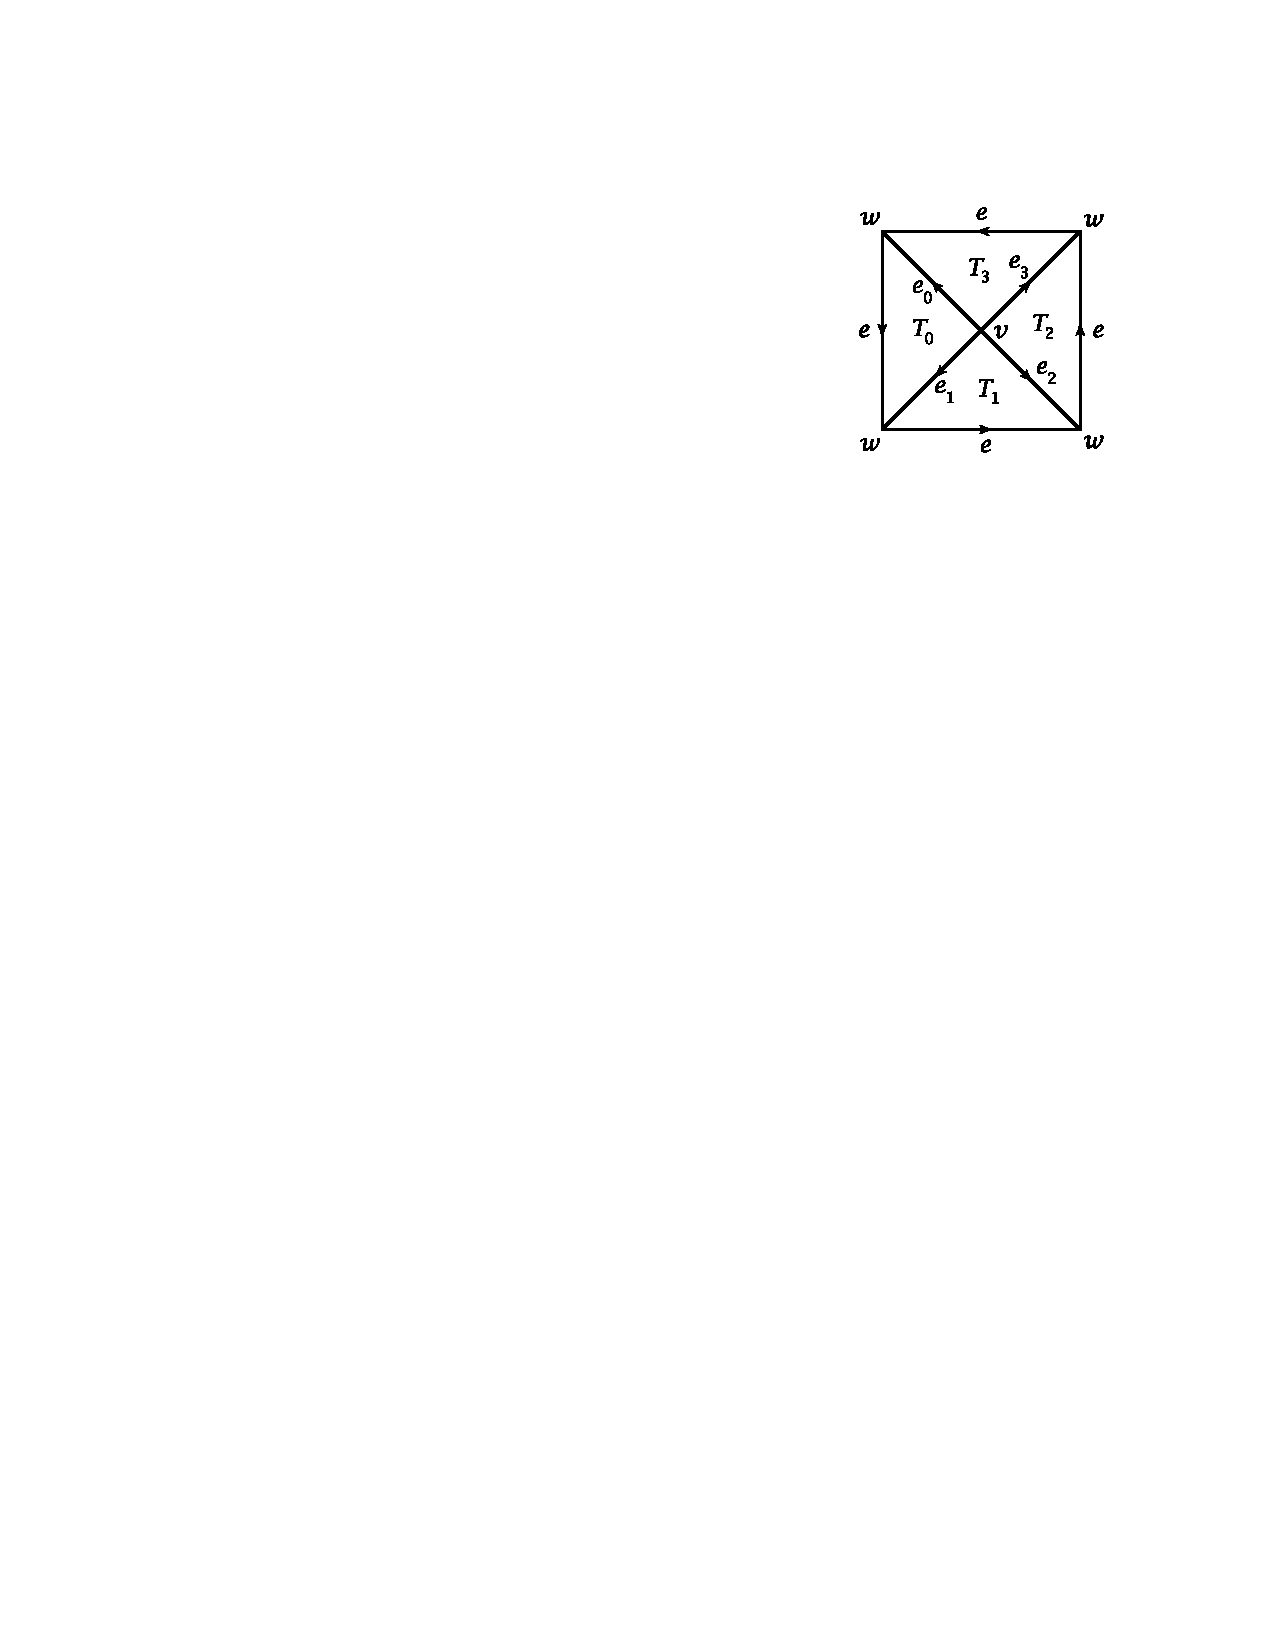
\includegraphics{cup-product}\]
This gives $X$ a $\Delta$-complex structure with $2$ vertices, $m+1$ edges, and $m$ $2$-simplices.\par
A generator $\alpha$ of $H^1(X;\Z/m\Z)$ is represented by a cocycle $\varphi$ assigning the value $1$ to the edge $e$, which generates $H_1(X)$. The condition that $\varphi$ be a cocycle means that \[\varphi(e_i)+\varphi(e)=\varphi(e_{i+1})\]
for all $i$, subscripts being taken mod $m$. So we may take $\varphi(e_i)=i\in\Z/m\Z$. Hence $(\varphi\cup\varphi)(T_i)=\varphi(e_i)\,\varphi(e)=i$. The map
$h:H^2(X;\Z/m\Z)\to\Hom(H^2(X;\Z/m\Z),\Z/m\Z)$ is an isomorphism by the universal coefficient theorem since $H^1(X;\Z/m\Z)=\Z/m\Z$ is free. The cocycle $\varphi\cup\varphi$ takes the value $0+1+\cdots+(m-1)=m(m-1)/2$ on $\sum_iT_i$, hence represents $m(m-1)/2$ times a generator $\beta$ of $H^2(X;\Z/m\Z)$. In $\Z/m\Z$ the sum $m(m-1)/2$ is $0$ if $m$ is odd and $k$ if $m=2k$. Thus, writing $\alpha^2$ for $\alpha\cup\alpha$, we have $\alpha^2=0$ if $m$ is odd and $\alpha^2=k\beta$ if $m=2k$.
\end{example}
The cup product formula $(\varphi\cup\psi)(\sigma)=\varphi(\sigma|[v_0,\cdots,v_k])\,\psi(\sigma|[v_{k},\cdots,v_{k+\ell}])$ also gives relative cup products
\[\begin{tikzcd}
H^k(X;R)\times H^\ell(X,A;R)\ar[r,"\cup"]&H^{k+\ell}(X,A;R)
\end{tikzcd}\]
\[\begin{tikzcd}
H^k(X,A;R)\times H^\ell(X;R)\ar[r,"\cup"]&H^{k+\ell}(X,A;R)
\end{tikzcd}\]
\[\begin{tikzcd}
H^k(X,A;R)\times H^\ell(X,A;R)\ar[r,"\cup"]&H^{k+\ell}(X,A;R)
\end{tikzcd}\]
since if $\varphi$ or $\psi$ vanishes on chains in $A$ then so does $\varphi\cup\psi$. There is a more general relative cup product
\[\begin{tikzcd}
H^k(X,A;R)\times H^\ell(X,B;R)\ar[r,"\cup"]&H^{k+\ell}(X,A\cup B;R)
\end{tikzcd}\]
when $A$ and $B$ are open subsets of $X$ or subcomplexes of the CW complex $X$. This is obtained in the following way. The absolute cup product restricts to a cup product $C^k(X,A;R)\times C^\ell(X,B;R)\to C^{k+\ell}(X,A+B;R)$ where $C^n(X,A+B;R)$ is the subgroup of $C^n(X;R)$ consisting of cochains vanishing on sums of chains in $A$ and chains in $B$. If $A$ and $B$ are open in $X$, the inclusions $C^n(X,A\cup B;R)֓\hookrightarrow C^n(X,A+B;R)$ induce isomorphisms on cohomology, via the five-lemma and the fact that the restriction maps $C_n(A\cup B;R)\to C_n(A+B;R)$ induce isomorphisms on cohomology as we saw in the discussion of excision in the previous section. Therefore the cup product $C^k(X,A;R)\times C^\ell(X,B;R)\to C^{k+\ell}(X,A+B;R)$ induces the desired relative cup product $H^k(X,A;R)\times H^\ell(X,B;R)\to H^{k+\ell}(X,A\cup B;R)$. This holds also if $X$ is a CW complex with $A$ and $B$ subcomplexes since here again the maps $C^n(A\cup B;R)\to C^n(A+B;R)$ induce isomorphisms on cohomology.
\begin{proposition}
For a map $f:X\to Y$, the inducedmaps $f^*:H^n(Y;R)\to H^n(X;R)$ satisfy $f^*(\alpha\cup\beta)=f^*(\alpha)\cup f^*(\beta)$, and similarly in the relative case.
\end{proposition}
\begin{proof}
This comes from the cochain formula $f^\flat(\varphi\cup\psi)=f^\flat(\varphi)\cup f^\flat(\psi)$:
\begin{align*}
(f^\flat\varphi\cup f^\flat\psi)&=f^\flat\varphi(\sigma|[v_0,\cdots,v_k])f^\flat\psi(\sigma|[v_k,\cdots,v_{k+\ell}])\\
&=\varphi(f\sigma|[v_0,\cdots,v_k])\,\psi(f\sigma|[v_k,\cdots,v_{k+\ell}])\\
&=(\varphi\cup\psi)(f\sigma)=f^\flat(\varphi\cup\psi)(\sigma).
\end{align*}
\end{proof}
The natural question of whether the cup product is commutative is answered by
the following:
\begin{theorem}
The identity $\alpha\cup\beta=(-1)^{k\ell}\beta\cup\alpha$ holds for all $\alpha\in H^k(X,A;R)$ and $\beta\in H^\ell(X,A;R)$, when $R$ is commutative.
\end{theorem}
Taking $\alpha=\beta$, this implies in particular that if $\alpha$ is an element of $H^k(X,A;R)$ with $k$ odd, then $2(\alpha\cup\alpha)=0$ in $H^{2k}(X,A;R)$, or more concisely, $2\alpha^2=0$. Hence if $H^{2k}(X,A;R)$ has no elements of order two, then $\alpha^2=0$. For example, if $X$ is the $2$-complex obtained by attaching a disk to $S^1$ by a map of degree $m$, then we can deduce that the square of a generator of $H^1(X;\Z/m\Z)$ is zero if $m$
is odd, and is either zero or the unique element of $H^2(X;\Z/m\Z)=\Z/m\Z$ of order two if $m$ is even. As we showed, the square is in fact nonzero when $m$ is even.
\begin{proof}
Consider first the case $A=\emp$. For cochains $\varphi\in C^k(X;R)$ and $\psi\in C^\ell(X;R)$ one can see from the definition that the cup products $\varphi\cup\psi$ and $\psi\cup\varphi$ differ only by a permutation of the vertices of $\Delta^{k+\ell}$. The idea of the proof is to study a particularly
nice permutation of vertices, namely the one that totally reverses their order. This has the convenient feature of also reversing the ordering of vertices in any face.\par
For a singular $n$ simplex $\sigma:[v_0,\cdots,v_n]\to X$, let $\widebar{\sigma}$ be the singular $n$-simplex obtained by preceding $\sigma$ by the linear homeomorphism of $[v_0,\cdots,v_n]$ reversing the order of the vertices. Thus $\widebar{\sigma}(v_i)=\sigma(v_{n-i})$. This reversal of vertices is the product of $n+(n-1)+\cdots+1=n(n + 1)/2$ transpositions of adjacent vertices, each of which reverses orientation of the $n$-simplex since it is a reflection across an $(n-1)$-dimensional hyperplane. So to take orientations into account we would expect that a sign $\eps_n=(-1)^{n(n+1)/2}$ ought to be inserted. Hence we define a homomorphism $\rho:C_n(X)\to C_n(X)$ by $\rho(\sigma)=\eps_n\widebar{\sigma}$.\par
We will show that $\rho$ is a chain map, chain homotopic to the identity, so it induces the identity on cohomology. From this the theorem quickly follows. Namely, the formulas
\[(\rho^*\varphi\cup\rho^*\psi)(\sigma)=\varphi(\eps_k\sigma|[v_k,\cdots,v_0])\,\psi(\eps_\ell\sigma|[v_{k+\ell},\cdots,v_{k}])\]
\[\rho^*(\psi\cup\varphi)(\sigma)=\eps_{k+\ell}\psi(\sigma|[v_{k+\ell},\cdots,v_k])\,\varphi(\sigma|[v_k,\cdots,v_{0}])\]
show that $\eps_k\eps_\ell(\rho^*\varphi\cup\rho^*\psi)=\eps_{k+\ell}\rho^*(\psi\cup\varphi)$, since we assume $R$ is commutative. A trivial calculation gives \[\eps_{k+\ell}=(-1)^{(k+\ell)(k+\ell+1)/2}=(-1)^{k(k+1)/2+\ell(\ell+1)/2+k\ell}=(-1)^{k\ell}\eps_k\eps_\ell,\] 
hence $\rho^*\varphi\cup\rho^*\psi=(-1)^{k\ell}\rho^*(\psi\cup\varphi)$. Since $\rho$ is chain homotopic to the identity, the $\rho^*$ disappears when we pass to cohomology classes, and so we obtain the desired formula $\alpha\cup\beta=(-1)^{k\ell}\beta\cup\alpha$.\par
The chain map property $\partial\rho=\rho\partial$ can be verified by calculating, for a singular $n$-simplex $\sigma$,
\begin{align*}
\partial\rho(\sigma)&=\eps_n\sum_i(-1)^i\sigma|[v_n,\cdots,\widehat{v}_{n-i},\cdots,v_0]\\
\rho(\partial\sigma)&=\rho\Big(\sum_i(-1)^i\sigma|[v_0,\cdots,\widehat{v}_i,\cdots,v_k]\Big)\\
&=\eps_{n-1}\sum_{i}(-1)^i\sigma|[v_k,\cdots,\widehat{v}_{n-i},\cdots,v_0]\\
&=\eps_{n-1}\sum_{i}(-1)^{n-i}\sigma|[v_k,\cdots,\widehat{v}_{n-i},\cdots,v_0]
\end{align*}
so the result follows from the easily checked identity $\eps_n=(-1)^n\eps_{n-1}$.\par
To define a chain homotopy between $\rho$ and the identity we are motivated by
the construction of the prism operator $h$ in the proof that homotopic maps induce the same homomorphism on homology. The main ingredient in the construction of $h$ was a subdivision of $\Delta^n\times I$ into $(n+1)$ simplices with vertices $v_i$ in $\Delta^n\times\{0\}$ and $w_i$ in $\Delta^n\times\{1\}$, the vertex $w_i$ lying directly above $v_i$. Using the same subdivision, and letting $\pi:\Delta^n\times I\to\Delta^n$ be the projection, we now define $P:C_n(X)\to C_{n+1}(X)$ by 
\[P(\sigma)=\sum_i(-1)^i\eps_{n-i}(\sigma\pi)|[v_0,\cdots,v_i,w_n,\cdots,w_i]\]
Thus the $w$ vertices are written in reverse order, and there is a compensating sign $\eps_{n-i}$. One can view this formula as arising from the $\Delta$-complex structure on $\Delta^n\times I$ in which the vertices are ordered $v_0,\cdots,v_n,w_n,\cdots,w_0$ rather than the more natural ordering $v_0,\cdots,v_n,w_0,\cdots,w_n$.\par
To show $\partial P+P\partial=\rho-\mathrm{id}$ we first calculate $\partial P$, leaving out $\sigma$'s and $\sigma\pi$'s for notational simplicity:
\begin{align*}
\partial P=&\sum_{j\leq i}(-1)^i(-1)^j\eps_{n-i}[v_0,\cdots,\widehat{v}_j,\cdots,v_i,w_n,\cdots,w_i]\\
&+\sum_{j\geq i}(-1)^i(-1)^{i+1+n-j}\eps_{n-i}[v_0,\cdots,v_i,w_n,\cdots,\widehat{w}_j,\cdots,w_i]
\end{align*}
The $j=i$ terms in these two sums give
\begin{align*}
\eps[w_n,\cdots,w_0]&+\sum_{i>0}\eps_{n-i}[v_0,\cdots,v_{i-1},w_n,\cdots,w_i]\\
&+\sum_{i<n}(-1)^{n+i+1}\eps_{n-i}[v_0,\cdots,v_i,w_{n},\cdots,w_{i+1}]-[v_0,\cdots,v_n]
\end{align*}
In this expression the two summation terms cancel since replacing $i$ by $i-1$ in the second sum produces a new sign $(-1)^{n+i}\eps_{n-i+1}=-\eps_{n-i}$. The remaining two terms $\eps_n[w_n,\cdots,w_0]$ and $-[v_0,\cdots,v_n]$ represent $\rho(\sigma)-\sigma$. So in order to show that $\partial P+P\partial=\rho-\mathrm{id}$, it remains to check that in the formula for $\partial P$ above, the terms with $j\neq i$ give $-P\partial$. Calculating $P\partial$ from the definitions, we have
\begin{align*}
P\partial&=\sum_{i<j}(-1)^i(-1)^j\eps_{n-i-1}[v_0,\cdots,v_i,w_n,\cdots,\widehat{w}_j,\cdots,w_i]\\
&+\sum_{i>j}(-1)^{i-1}(-1)^j\eps_{n-i}[v_0,\cdots,\widehat{v}_j,\cdots,v_i,w_n,\cdots,w_i]
\end{align*}
Since $\eps_{n-i}=(-1)^{n-i}\eps_{n-i-1}$, this finishes the verification that $\partial P+P\partial=\rho-\mathrm{id}$, and so the theorem is proved when $A=\emp$. The proof also applies when $A\neq\emp$ since the maps $\rho$ and $P$ take chains in $A$ to chains in $A$, so the dual homomorphisms $\rho^*$ and
$P^*$ act on relative cochains.
\end{proof}
\subsection{The Cohomology Ring}
We simply define $H^*(X;R)$ to be the direct sum of the groups $H^n(X;R)$. For example, the calculations in Example~\ref{cup prod eg} above show that $H^*(\RP^2;\Z/2\Z)$ consists of the polynomials $a_0+a_1\alpha+a_2\alpha^2$ with coefficients $a_i\in\Z/2\Z$, so $H^*(\RP^2;\Z/2\Z)$ is the quotient $\Z/2\Z[\alpha]/(\alpha^3)$.\par
This example illustrates how $H^*(X;R)$ often has a more compact description
than the sequence of individual groups $H^n(X;R)$, so there is a certain economy in the change of scale that comes from regarding all the groups $H^n(X;R)$ as part of a single object $H^*(X;R)$.\par
Adding cohomology classes of different dimensions to form $H^*(X;R)$ is a convenient formal device, but it has little topological significance. One always regards the cohomology ring as a \textbf{graded ring}: a ring $A$ with a decomposition as a sum $\bigoplus_{k\geq 0}A_k$ of additive subgroups $A_k$ such that the multiplication takes $A_k\times A_\ell$ to $A_{k+\ell}$. To indicate that an element $a\in A$ lies in $A_k$ we write $|a|=k$. This applies in particular to elements of $H^k(X;R)$. We will use the term \textit{dimension} for $|a|$ and avoids potential confusion with the degree of a polynomial.\par
A graded ring satisfying the commutativity property $ab=(-1)^{|a||b|}ba$, is usually called simply commutative in the context of algebraic topology, in spite of the potential for misunderstanding. In the older literature one finds
less ambiguous terms such as graded commutative, anticommutative, or skew commutative.
\begin{example}[\textbf{Polynomial Rings}]
Among the simplest graded rings are polynomial rings $R[\alpha]$ and their truncated versions $R[\alpha]/(\alpha^n)$, consisting of polynomials of degree less than $n$. The example we have seen is $H^*(\RP^2;\Z/2\Z)=\Z/2\Z[\alpha]/(\alpha^3)$. More generally we will show that $H^*(\RP^n;\Z/2\Z)=\Z/2\Z[\alpha]/(\alpha^{n+1})$ and $H^*(\RP^\infty;\Z/2\Z)=\Z/2\Z[\alpha]$. In these cases $|\alpha|=1$. We will also show that $H^*(\CP^n;\Z)=\Z[\alpha]/(\alpha^{n+1})$ and $H^*(\CP^\infty;\Z)=\Z[\alpha]$ with $|\alpha|=2$. The analogous results for quaternionic projective spaces are also valid, with $|\alpha|=4$. The coefficient ring $\Z$ in the complex and quaternionic cases could be replaced by any commutative ring $R$, but not for $\RP^n$ and $\RP^\infty$ since a polynomial ring $R[\alpha]$ is strictly commutative, so for this to be a commutative ring in the graded sense we must have either $|\alpha|$ even or $2=0$ in $R$.\par
Polynomial rings in several variables also have graded ring structures, and these graded rings can sometimes be realized as cohomology rings of spaces. For example, $\Z/2\Z[\alpha_1,\cdots,\alpha_n]$ is $H^*(X;\Z/2\Z)$ for $X$ the product of $n$ copies of $\RP^\infty$, with $|\alpha_i|=1$ for each $i$, as we will see.
\end{example}
\begin{example}
The isomorphism $H^*(\coprod_\alpha X_\alpha;R)\stackrel{\cong}{\longrightarrow}\prod_\alpha H^*(X_\alpha;R)$
whose coordinates are induced by the inclusions $i_\alpha:X_\alpha\hookrightarrow\coprod_\alpha X_\alpha$ is a ring isomorphism
with respect to the usual coordinatewise multiplication in a product ring, because each coordinate function $i^*_\alpha$ is a ring homomorphism. Similarly for a wedge sum the isomorphism $\widetilde{H}^*(\bigvee_\alpha X_\alpha;R)\cong\prod_\alpha\widetilde{H}^*(X_\alpha;R)$ is a ring isomorphism. Here we take reduced cohomology to be cohomology relative to a basepoint, and we use relative cup products. We should assume the basepoints $x_\alpha\in X_\alpha$ are deformation retracts of neighborhoods, to be sure that the claimed isomorphism does indeed hold.\par
This product ring structure for wedge sums can sometimes be used to rule out
splittings of a space as a wedge sum up to homotopy equivalence. For example, consider $\CP^2$, which is $S^2$ with a cell $e^4$ attached by a certain map $f:S^3\to S^2$. Using homology or just the additive structure of cohomology it is impossible to conclude that $\CP^2$ is not homotopy equivalent to $S^2\vee S^4$, and hence that $f$ is not homotopic to a constant map. However, with cup products we can distinguish these two spaces since the square of each element of $H^2(S^2\vee S^4;\Z)$ is zero in view of the ring isomorphism $\widetilde{H}^*(S^2\vee S^4;\Z)\cong\widetilde{H}^*(S^2;\Z)\oplus\widetilde{H}^*(S^4;\Z)$, but the square of a generator of $H^2(\CP^2;\Z)$ is nonzero since $H^*(\CP^2;\Z)\cong \Z[\alpha]/(\alpha^3)$.\par
More generally, cup products can be used to distinguish infinitely many different homotopy classes of maps $S^{4n-1}\to S^{2n}$ for all $n\geq 1$. This is systematized in the notion of the \textbf{Hopf invariant}.
\end{example}
\subsection{A K\"unneth Formula}
To begin, we define the \textbf{cross product}, or \textbf{external cup product} as it is sometimes called. This is the map
\[\begin{tikzcd}
H^*(X;R)\times H^*(Y;R)\ar[r,"\times"]&H^*(X\times Y;R)
\end{tikzcd}\]
given by $a\times b=p_1^*(a)\cup p^*_2(b)$ where $p_1$ and $p_2$ are the projections of $X\times Y$ onto $X$ and $Y$. Since cup product is distributive, the cross product is bilinear, that is, linear in each variable separately. However, a bilinear map is rarely a homomorphism, so it could hardly be an isomorphism. Fortunately there is a nice algebraic solution to this problem, and that is to replace the direct product $H^*(X;R)\times H^*(Y;R)$ by the tensor product $H^*(X;R)\otimes_R H^*(Y;R)$.\par
Let us review some basic properties of tensor products
\begin{itemize}
\item[$(1)$]$A\otimes B=B\otimes A$.
\item[$(2)$]$(\bigoplus_iA_i)\otimes B=\bigoplus_i(A_i\otimes B)$.
\item[$(3)$]$(A\otimes B)\otimes C=A\otimes(B\otimes C)$.
\item[$(4)$]$\Z\otimes A=A$.
\item[$(5)$]$\Z/n\Z\otimes A=A/nA$.
\item[$(6)$]A pair of homomorphisms $f:A\to A'$ and $g:B\to B'$ induces a homomorphism $f\otimes g:A\otimes B\to A'\otimes B'$ via $(f\otimes g)(a\otimes b)=f(a)\otimes g(b)$.
\item[$(7)$]A bilinear map $\varphi:A\times B\to C$ induces a homomorphism $A\otimes B\to C$ sending $a\otimes b$ to $\varphi(a,b)$.
\end{itemize}
We will restrict attention to the case that $R$ is commutative in what follows. It is an easy algebra exercise to see that $A\otimes_RB=A\otimes_\Z B$ when $R$ is $\Z/m\Z$ or $\Q$. But in general $A\otimes_RB$ is not the same as $A\otimes R$. For example, if $R=\Q(\sqrt{2})$, which is a $2$-dimensional vector space over $\Q$, then $R\otimes_RR=R$ but $R\otimes R$ is a $4$-dimensional vector space over $\Q$.\par
Property $(7)$ of tensor products guarantees that the cross product as defined above gives rise to a homomorphism of $R$-modules
\[\begin{tikzcd}
H^*(X;R)\otimes_RH^*(Y;R)\ar[r,"\times"]&H^*(X\times Y;R)
\end{tikzcd},\quad a\otimes b\mapsto a\times b\]
which we shall also call cross product. This map becomes a ring homomorphism if
we define the multiplication in a tensor product of graded rings by $(a\otimes b)(c\otimes d)=(-1)^{|b||c|}ac\otimes bd$ where $|x|$ denotes the dimension of $x$. Namely, if we denote the cross product map by $\mu$ and we define $(a\otimes b)(c\otimes  d)=(-1)^{|b||c|}ac\otimes bd$, then
\begin{align*}
\mu\big((a\otimes b)(c\otimes d)\big)&=(-1)^{|b||c|}\mu(ac\otimes bd)\\
&=(-1)^{|b||c|}(a\cup c)\times(b\cup d)\\
&=(-1)^{|b||c|}p_1^*(a\cup c)\cup p_2^*(b\cup d)\\
&=(-1)^{|b||c|}p_1^*(a)\cup p_1^*(c)\cup p_2^*(b)\cup p_2^*(d)\\
&=p_1^*(a)\cup p_2^*(b)\cup p_1^*(c)\cup p_2^*(d)\\
&=(a\times b)(b\times d)=\mu\big(a\otimes b\big)\mu(b\otimes d)
\end{align*}
\begin{theorem}\label{homology prod}
The cross product $H^*(X;R)\otimes_RH^*(Y;R)\to H^*(X\times Y;R)$ is an isomorphism of rings if $X$ and $Y$ are CW complexes and $H^k(Y;R)$ is a finitely generated free $R$ module for all $k$.
\end{theorem}
\begin{example}
The exterior algebra $\bigwedge_R[\alpha_1,\cdots,\alpha_n]$ is the graded tensor product over $R$ of the one-variable exterior algebras $\bigwedge_R[\alpha_i]$ where the $\alpha_i$'s have odd dimension. The K\"unneth formula then gives an isomorphism $H^*(S^{k_1}\times\cdots\times S^{k_n};\Z)\cong\bigwedge_\Z[\alpha_1,\cdots,\alpha_n]$ if the dimensions $k_i$ are all odd. With some $k_i$'s even, one would have the tensor product of an exterior algebra for the odd-dimensional spheres and truncated polynomial rings $\Z[\alpha]/(\alpha^2)$ for the even-dimensional spheres. Of course, $\bigwedge_Z[\alpha]$ and $\Z[\alpha]/(\alpha^2)$ are isomorphic as rings, but when one takes tensor products in the graded sense it becomes important to distinguish them as graded rings, with $\alpha$ odd-dimensional in $\bigwedge_\Z[\alpha]$ and even-dimensional in $\Z[\alpha]/(\alpha^2)$. These remarks apply more generally with any coefficient ring $R$ in place of $\Z$, though when $R=\Z/2\Z$ there is no need to distinguish between the odd-dimensional and even-dimensional cases since signs become irrelevant.
\end{example}
The idea of the proof of the theorem will be to consider, for a fixed CW complex $Y$, the functors
\[h^n(X,A)=\bigoplus_i\big(H^i(X,A;R)\otimes_R H^{n-i}(Y;R)\big)\]
\[k^n(X,A)=H^n(X\times Y,A\times Y;R)\]
The cross product, or a relative version of it, defines a map $\mu:h^n(X,A)\to k^n(X,A)$ which we would like to show is an isomorphism when $X$ is a CW complex and $A=\emp$. We will show:
\begin{itemize}
\item[$(a)$]$h^*$ and $k^*$ are cohomology theories on the category of CW pairs.
\item[$(b)$]$\mu$ is a natural transformation: It commutes with induced homomorphisms and with coboundary homomorphisms in long exact sequences of pairs.
\end{itemize}
It is obvious that $\mu:h^n(X)\to k^n(X)$ is an isomorphism when $X$ is a point since it is just the scalar multiplication map $R\otimes_RH^n(Y;R)\to H^n(Y;R)$. The following general fact will then imply the theorem.
\begin{proposition}
If a natural transformation between unreduced cohomology theories on the category of CW pairs is an isomorphism when the CW pair is $($point ,$\emp$$)$,
then it is an isomorphism for all CW pairs.
\end{proposition}
\begin{proof}
Let $\mu:h^*(X,A)\to k^*(X,A)$ be the natural transformation. By the five-lemma
it will suffice to show that $\mu$ is an isomorphism when $A=\emp$.\par
First we do the case of finite-dimensional $X$ by induction on dimension. The
induction starts with the case that $X$ is $0$-dimensional, where the result holds by hypothesis and by the axiom for disjoint unions. For the induction step, $\mu$ gives a map between the two long exact sequences for the pair $(X^n,X^{n-1})$, with commuting squares since $\mu$ is a natural transformation. The five-lemma reduces the inductive step to showing that $\mu$ is an isomorphism for $(X,A)=(X^n,X^{n-1})$. Let $\Phi:\coprod_\alpha(D^n_\alpha,\partial D^n_\alpha)\to (X^n,X^{n-1})$ be a collection of characteristic maps for all the $n$-cells of $X$. By excision, $\Phi$ is an isomorphism for $h^*$ and $k^*$, so by naturality it suffices to show that $\mu$ is an isomorphism for $(X,A)=\coprod_\alpha(D^n_\alpha,\partial D^n_\alpha)$. The axiom for disjoint
unions gives a further reduction to the case of the pair $(D^n,\partial D^n)$. Finally, this case follows by applying the five-lemma to the long exact sequences of this pair, since $D^n$ is contractible and hence is covered by the $0$-dimensional case, and $\partial D^n$ is $(n-1)$-dimensional.\par
The case that $X$ is infinite-dimensional reduces to the finite-dimensional case by a telescope argument.
\end{proof}
\begin{proof}[Proof of Theorem~\ref{homology prod}]
It remains to check that $h^*$ and $k^*$ are cohomology theories, and that $\mu$ is a natural transformation. Since we are dealing with unreduced cohomology theories there are four axioms to verify.
\begin{itemize}
\item[$(1)$]Homotopy invariance: $f\simeq g$ implies $f^*=g^*$. This is obvious for both $h^*$ and $k^*$.
\item[$(2)$]Excision: $h^*(X,A)=h^*(B,A\cap B)$ for $A$ and $B$ subcomplexes of the CW complex $X=A\cup B$. This is obvious, and so is the corresponding statement for $k^*$ since $(A\times Y)\cup(B\times Y)=(A\cup B)\times Y$ and $(A\times Y)\cap (B\times Y)=(A\cap B)\times Y$.
\item[$(3)$]The long exact sequence of a pair. This is a triviality for $k^*$, but a few words of explanation are needed for $h^*$, where the desired exact sequence is obtained in two steps. For the first step, tensor the long exact sequence of ordinary cohomology groups for a pair $(X,A)$ with the free $R$-module $H^n(Y;R)$, for a fixed $n$. This yields another exact sequence because $H^n(Y;R)$ is free, hence flat. The second step is to let $n$ vary, taking a direct sum of the previously constructed exact sequences for each $n$, with the $n$-th exact sequence shifted up by $n$ dimensions.
\item[$(4)$]Disjoint unions. Again this axiom obviously holds for $k^*$, but some justification is required for $h^*$. What is needed is the algebraic fact that there is a canonical isomorphism $(\prod_\alpha M_\alpha)\otimes_RN=\prod_\alpha(M_\alpha\otimes_RN)$ for $R$ modules $M_\alpha$ and a finitely generated free $R$ module $N$. Since $N$ is a direct product of finitely many copies $R_\beta$ of $R$, $M_\alpha\otimes_RN$ is a direct product of corresponding copies $M_{\alpha\beta}=M_\alpha\otimes_RR_\beta$ of $M_\alpha$ and the desired relation becomes $\prod_\beta\prod_\alpha M_{\alpha\beta}=\prod_\alpha\prod_\beta M_{\beta\alpha}$, which is obviously
true.
\end{itemize}
Finally there is naturality of $\mu$ to consider. Naturality with respect to maps between spaces is immediate from the naturality of cup products. Naturality with respect to coboundary maps in long exact sequences is commutativity of the following square:
\[\begin{tikzcd}
H^k(A;R)\times H^\ell(Y;R)\ar[r,"\delta\times\mathrm{id}"]\ar[d,"\times"]&H^{k+1}(X,A;R)\times H^\ell(Y;R)\ar[d,"\times"]\\
H^{k+\ell}(A\times Y;R)\ar[r,"\delta"]&H^{k+\ell+1}(X\times Y,A\times Y;R)
\end{tikzcd}\]
To check this, start with an element of the upper left product, represented by cocycles $\varphi\in C^k(A;R)$ and $\psi\in C^\ell(Y;R)$. Extend $\varphi$ to a cochain $\widetilde{\varphi}\in C^k(X;R)$. Then the pair $(\varphi,\psi)$ maps rightward to $(\delta\widetilde{\varphi},\psi)$ and then downward to $p^\flat_1(\delta\widetilde{\varphi})\cup p^\flat_2(\psi)$. Going the other way around the square, $(\varphi,\psi)$ maps downward to $p^\flat_1(\varphi)\cup p^\flat_2(\psi)$ and then rightward to $\delta(p^\flat_1(\widetilde{\varphi})\cup p^\flat_2(\psi))$ since $p^\flat_1(\varphi)\cup p^\flat_2(\psi)$ extends $p^\flat_1(\widetilde{\varphi})\cup p^\flat_2(\psi)$ over
$X\times Y$. Finally, $\delta\big(p^\flat_1(\widetilde{\varphi})\cup p^\flat_2(\psi)\big)=p^\flat_1(\delta\widetilde{\varphi})\cup p^\flat_2(\psi)$  since $\delta\psi=0$.
\end{proof}
It is sometimes important to have a relative version of the K\"unneth formula. The relative cross product is
\[\begin{tikzcd}
H^*(X,A;R)\otimes_R H^*(Y,B;R)\ar[r,"\times"]&H^*(X\times Y,A\times Y\cup X\times B;R)
\end{tikzcd}\]
for CW pairs $(X,A)$ and $(Y,B)$, defined just as in the absolute case by $a\times b=p^*_1(a)\cup p^*_2(b)$ where $p^*_1(a)\in H^*(X\times Y,A\times Y;R)$ and $p^*_1(a)\in H^*(X\times Y,X\times B;R)$.
\begin{theorem}\label{Kunneth formula}
For CW pairs $(X,A)$ and $(Y,B)$ the cross product homomorphism 
\[\begin{tikzcd}
H^*(X,A;R)\otimes_RH^*(Y,B;R)\ar[r,"\times"]&H^*(X\times Y,A\times Y\cup X\times B;R)
\end{tikzcd}\]
is an isomorphism of rings if $H^k(Y,B;R)$ is a finitely generated free $R$ module for each $k$.
\end{theorem}
\begin{proof}
The case $B=\emp$ was covered in the course of the proof of the absolute case, so it suffices to deduce the case $B\neq\emp$ from the case $B=\emp$.\par 
The following commutative diagram shows that collapsing $B$ to a point reduces
the proof to the case that $B$ is a point:
\[\begin{tikzcd}
H^*(X,A)\otimes_RH^*(Y,B)\ar[d,"\times"]&H^*(X,A)\otimes_RH^*(Y/B,B/B)\ar[l,swap,"\cong"]\ar[d,"\times"]\\
H^*(X\times Y,A\times Y\cup X\times B;R)&H^*(X\times(Y/B),A\times(Y/B)\cup X\times(B/B))\ar[l,swap,"\cong"]
\end{tikzcd}\]
The lower map is an isomorphism since the quotient spaces 
\[(X\times Y)/(A\times Y\cup X\times B)\And\big(X\times(Y/B)\big)/\big(A\times(Y/B)\cup X\times(B/B)\big)\]
are the same.\par
In the case that $B$ is a point $y_0\in Y$, consider the commutative diagram
\[\begin{tikzcd}
H^*(X,A)\otimes_RH^*(Y,y_0)\ar[r]\ar[dd,"\times"]&H^*(X,A)\otimes_RH^*(Y)\ar[r]\ar[dd,"\times"]&H^*(X,A)\otimes_RH^*(y_0)\ar[d,"\times"]\\
&&H^*(X\times y_0,A\times y_0)\\
H^*(X\times Y,X\times y_0\cup A\times Y)\ar[r]&H^*(X\times Y,A\times Y)\ar[r]\ar[ru]&H^*(X\times y_0\cup A\times Y,A\times Y)\ar[u,"\cong"]
\end{tikzcd}\]
Since $y_0$ is a retract of $Y$, the upper row of this diagramis a split short exact sequence (the second map has a right-inverse). The lower row is the long exact sequence of a triple, and it too is a split short exact sequence since $(X\times y_0,A\times y_0)$ is a retract of $(X\times Y,A\times Y)$. The middle and right cross product maps are isomorphisms by the case $B=\emp$ since $H^k(Y;R)$ is a finitely generated free $R$ module if $H^k(Y,y_0;R)$ is. The five-lemma then implies that the left-hand cross product map is an isomorphism as well.
\end{proof}
The relative cross product for pairs $(X,x+0)$ and $(Y,y_0)$ gives a reduced cross product
\[\begin{tikzcd}
\widetilde{H}^*(X;R)\otimes_R\widetilde{H}^*(Y;R)\ar[r,"\times"]&\widetilde{H}^*(X\wedge Y;R)
\end{tikzcd}\]
where $X\wedge Y$ is the smash product $X\times Y/(X\times\{y_0\}\cup\{x_0\}\times Y)$. The preceding theorem implies that this reduced cross product is an isomorphism if $\widetilde{H}^*(X;R)$ or $\widetilde{H}^*(Y;R)$ is free and finitely generated in each dimension. For example, we have isomorphisms $\widetilde{H}^n(X;R)=\widetilde{H}^{n+k}(X\wedge S^k;R)$ via cross product with a generator of $H^k(S^k;R)=R$. The space $X\wedge S^k$ is the $k$-fold reduced suspension $imequm^kX$ of $X$. so we see that the suspension isomorphisms $\widetilde{H}^n(X;R)=\widetilde{H}^{n+k}(\sum^kX;R)$ derivable by elementary exact sequence arguments can also be obtained via cross product with a generator of $\widetilde{H}^*(S^k;R)$.
\subsection{Spaces with Polynomial Cohomology}
Earlier in this section we mentioned that projective spaces provide examples of
spaces whose cohomology rings are polynomial rings. Here is the precise statement:
\begin{theorem}
$H^*(\RP^n;\Z/2\Z)\cong\Z/2\Z[\alpha]/(\alpha^{n+1})$ and $H^*(\RP^{\infty}; \Z/2\Z)\cong\Z/2\Z[\alpha]$, where $|\alpha|=1$. In the complex case, $H^*(\CP^n;\Z)\cong\Z[\alpha]/(\alpha^{n+1})$ and $H^*(\CP^\infty;\Z)\cong\Z[\alpha]$ where $|\alpha|=2$.
\end{theorem}
\begin{proof}
Let us do the case of $\RP^n$ first. To simplify notation we abbreviate $\RP^n$ to $\P^n$ and \textbf{we let the coefficient group $\Z/2\Z$ be implicit}. Since the inclusion $P^{n-1}\hookrightarrow\P^n$ induces an isomorphism on $H^i$ for $i\leq n-1$ (since we use $\Z/2\Z$ coefficient, the differentials are all zero), it suffices by induction on $n$ to show that the cup product of a generator of $H^{n-1}(\P^n)$ with a generator of $H^1(\P^n)$ is a generator of $H^n(\P^n)$. It will be no more work to show more generally that the cup product of a generator of $H^i(\P^n)$ with a generator of $H^{n-1}(\P^n)$ is a generator of $\H^n(\P^n)$. As a further notational aid, we let $j=n-i$, so $i+j=n$.\par
The proof uses some of the geometric structure of $\P^n$. Recall that $\P^n$ consists of nonzero vectors $(x_0,\cdots,x_n)\in\R^{n+1}$ modulo multiplication by nonzero scalars. Inside $\P^n$ is a copy of $\P^i$ represented by vectors whose last $j$ coordinates $x_{i+1},\cdots,x_n$ are zero. We also have a copy of $\P^j$ represented by points whose first $i$ coordinates $x_0,\cdots,x_{i-1}$ are zero. The intersection $\P^i\cap\P^j$ is a single point $p$, represented by vectors whose only nonzero coordinate is $x_i$. Let $U$ be the subspace of $\P^n$ represented by vectors with nonzero coordinate $x_i$. Each point in $U$ may be represented by a unique vector with $x_i=1$ and the other $n$ coordinates arbitrary, so $U$ is homeomorphic to $\R^n$, with $p$ corresponding to $0$ under this homeomorphism. We can write this $\R^n$ as $\R^i\times\R^j$, with $\R^i$ as the coordinates $x_0,\cdots,x_{i-1}$ and $\R^j$ as the coordinates $x_{i+1},\cdots,x_n$.\par
Consider the diagram
\begin{equation}\label{coeff ring-1}
\begin{tikzcd}
H^i(\P^n)\times H^j(\P^n)\ar[rr,"\cup"]&&H^n(\P^n)\\
H^i(\P^n,\P^n-\P^j)\times H^j(\P^n,\P^n-\P^i)\ar[rr,"\cup"]\ar[u]\ar[d]&&H^n(\P^n,\P^n-\{p\})\ar[u]\ar[d]\\
H^i(\R^n,\R^n-\R^j)\times H^j(\R^n,\R^n-\R^i)\ar[rr,"\cup"]&&H^n(\R^n,\R^n-\{0\})\\
\end{tikzcd}
\end{equation}
which commutes by naturality of cup product. We will show that the four vertical maps are isomorphisms and that the lower cup product map takes generator cross generator to generator. Commutativity of the diagram will then imply that the upper cup product map also takes generator cross generator to generator.\par
The lower map in the right column is an isomorphism by excision. For the upper
map in this column, the fact that $\P^n-\{p\}$ deformation retracts to a $\P^{n-1}$ gives an isomorphism $H^n(\P^n,\P^n-\{p\})\cong H^n(\P^n,\P^{n-1})$ via the five-lemma applied to the long exact sequences for these pairs. And $H^n(\P^n,\P^{n-1})\cong H^n(\P^n)$ by cellular cohomology.\par
To see that the vertical maps in the left column of $(\ref{coeff ring-1})$ are isomorphisms we will use the following commutative diagram:
\begin{equation}\label{coeff ring-2}
\begin{tikzcd}
H^i(\P^n)\ar[d]&H^i(\P^n,\P^{i-1})\ar[l]\ar[d]&H^i(\P^n,\P^n-\P^j)\ar[d]\ar[l]\ar[r]&H^i(\R^n,\R^n-\R^j)\ar[d]\\
H^i(\P^i)&H^i(\P^i,\P^{i-1})\ar[l]&H^i(\P^i,\P^i-\{p\})\ar[l]\ar[r]&H^i(\R^i,\R^i-\{0\})\\
\end{tikzcd}
\end{equation}
If we can show all these maps are isomorphisms, then the same argument will apply with $i$ and $j$ interchanged, and the vertical maps in the left column of $(\ref{coeff ring-1})$ will be isomorphisms.\par
The left-hand square in $(\ref{coeff ring-2})$ consists of isomorphisms by cellular cohomology. The right-hand vertical map is obviously an isomorphism. The lower right horizontal map is an isomorphism by excision, and the map to the left of this is an isomorphism since $\P^i-\{p\}$ deformation retracts onto $\P^{i-1}$. The remaining maps will be isomorphisms if the middle map in the upper row is an isomorphism. And this map is indeed an isomorphism because $\P^n-\P^j$ deformation retracts onto $\P^{i-1}$ by the following argument.\par
The subspace $\P^n-\P^j\sub \P^n$ consists of points represented by vectors $v=(x_0,\cdots,x_n)$ with at least one of the coordinates $x_0,\cdots,x_{i-1}$ nonzero. The formula $f_t(v)=(x_0,\cdots,x_{i-1},tx_i,\cdots,tx_n)$ for $t$ decreasing from $1$ to $0$ gives a well-defined deformation retraction of $P^n-P^j$ onto $P^{i-1}$ since $f_t(\lambda v)=\lambda f_t(v)$ for scalars $\lambda\in\R$. ($f_t$ is well-defined since $f_t(x)\neq 0$ for $x\in\P^n-\P^j$, for $x\in\P^n$, this is not a homotopy since it touches $0$.)\par
The cup product map in the bottom row of $(\ref{coeff ring-1})$ is equivalent to the cross product $H^i(I^i,\partial I^i)\times H^j(I^j,\partial I^j)\to H^n(I^n,\partial I^n)$, where the cross product of generators is a generator by the relative form of the K\"unneth formula in Theorem~\ref{Kunneth formula}. Alternatively, if one wishes to use only the absolute K\"unneth formula, the cross product for cubes is equivalent to the cross product $H^i(S^i)\times H^j(S^j)\to H^n(S^i\times S^j)$ by means of the quotient maps $I^i\to S^i$ and $I^j\to S^j$ collapsing the boundaries of the cubes to points.\par
This finishes the proof for $\RP^n$. The case of $\RP^\infty$ follows from this since the inclusion $\RP^n֓\hookrightarrow\RP^\infty$ induces isomorphisms on $H^i(-;\Z/2\Z)$ for $i\leq n$ by cellular cohomology.\par
Complex projective spaces are handled in precisely the same way, using $\Z$ coefficients and replacing each $H^k$ by $H^{2k}$ and $\R$ by $\C$.
\end{proof}
There are also quaternionic projective spaces $\H\mathrm{P}^n$ and $\H\mathrm{P}^\infty$, defined exactly as in the complex case, with CW structures of the form $e^0\cup e^4\cup e^8\cup\cdots$. The cup
product structure in quaternionic projective spaces is just like that in complex projective spaces, except that the generator is $4$-dimensional:
\[H^*(\H\mathrm{P}^\infty;\Z)\cong\Z[\alpha]\And H^*(\H\mathrm{P}^n;\Z)\cong\Z[\alpha]/(\alpha^{n+1}),\text{ with }|\alpha|=4.\]
The same proof as in the real and complex cases works here as well.\par
The cup product structure for $\RP^\infty$ with $\Z$ coefficients can easily be deduced from the cup product structure with $\Z/2\Z$ coefficients, as follows. In general, a ring homomorphism $R\to S$ induces a ring homomorphism $H^*(X,A;R)\to H^*(X,A;S)$. In the case of the projection $\Z\to\Z/2\Z$ we get for $\RP^\infty$ an induced chain map of cellular cochain complexes with $\Z$ and $\Z/2\Z$ coefficients:
\[\begin{tikzcd}
\cdots&\Z\ar[l]\ar[d]&\Z\ar[l,swap,"2"]\ar[d]&\Z\ar[l,swap,"0"]\ar[d]&\Z\ar[l,swap,"2"]\ar[d]&\Z\ar[l,swap,"0"]\ar[d]&0\ar[l]\\
\cdots&\Z/2\Z\ar[l]&\Z/2\Z\ar[l,swap,"0"]&\Z/2\Z\ar[l,swap,"0"]&\Z/2\Z\ar[l,swap,"0"]&\Z/2\Z\ar[l,swap,"0"]&0\ar[l]
\end{tikzcd}\]
From this we see that the ring homomorphism $H^*(\RP^\infty;\Z)\to H^*(\RP^\infty;\Z/2\Z)$ is injective in positive dimensions, with image the even-dimensional part of $H^*(\RP^\infty;\Z/2\Z)$. Alternatively, this could be deduced from the universal coefficient theorem. Hence we have $H^*(\RP^\infty;\Z)\cong\Z[\alpha]/(2\alpha)$ with $|\alpha|=2$.\par
The cup product structure in $H^*(\RP^n;\Z)$ can be computed in a similar fashion, though the description is a little cumbersome:
\[H^*(\RP^{2k};\Z)\cong\Z[\alpha](2\alpha,\alpha^{k+1}),\ |\alpha|=2.\]
\[H^*(\RP^{2k+1};\Z)\cong\Z[\alpha,\beta](2\alpha,\alpha^{k+1},\beta^2,\alpha\beta),\ |\alpha|=2,|\beta|=2k+1.\]
Here $\beta$ is a generator of $H^{2k+1}(\RP^{2k+1};\Z)=\Z$. From this calculation we see that the rings $H^*(\RP^{2k+1};\Z)$ and $H^*(\RP^{2k}\vee S^{2k+1};\Z)$ are isomorphic, though with $\Z/2\Z$ coefficients this is no longer true, as the generator $\alpha\in H^1(\RP^{2k+1};\Z/2\Z)$ has $\alpha^{2k+1}\neq0$, while $\alpha^{2k+1}=0$ for the generator $\alpha\in H^1(\RP^{2k}\vee S^{2k+1};\Z/2\Z)$.
\begin{example}
Combining the calculation $H^*(\RP^\infty;\Z/2\Z)\cong\Z/2\Z[\alpha]$ with the K\"unneth formula, we see that $H^*(\RP^\infty\times\RP^\infty;\Z/2\Z)$ is isomorphic to $\Z/2\Z[\alpha_1]\otimes\Z/2\Z[\alpha_2]$, which is just the polynomial ring $\Z/2\Z[\alpha_1,\alpha_2]$. More generally it follows by induction that for a product of $n$ copies of $\RP^\infty$, the $\Z/2\Z$ cohomology is a polynomial ring in $n$ variables. Similar remarks apply to $\CP^\infty$ and $\H\mathrm{P}^\infty$ with coefficients in $\Z$ or any commutative ring.
\end{example}
The following theorem of Hopf is a nice algebraic application of the cup product structure in $H^*(\RP^n\times\RP^n;\Z/2\Z)$.
\begin{theorem}
If $\R^n$ has the structure of a division algebra over the scalar field $\R$,
then $n$ must be a power of $2$.
\end{theorem}
\begin{proof}
For a division algebra structure on $\R^n$ the multiplication maps $x\mapsto ax$ and $x\mapsto xa$ are linear isomorphisms for each nonzero $a$, so the multiplication map $\R^n\times\R^n\to\R^n$ induces a map $h:\RP^{n-1}\times\RP^{n-1}\to\RP^{n-1}$ which is a homeomorphism when restricted to each subspace $\RP^{n-1}\times\{y\}$ and $\{x\}\times\RP^{n-1}$. The map $h$ is continuous since it is a quotient of the multiplication map which is bilinear and hence continuous.\par
The induced homomorphism $h^*$ on $\Z/2\Z$-cohomology is a ring homomorphism
$\Z/2\Z[\alpha]/(\alpha^n)\to\Z/2\Z[\alpha_1,\alpha_2]/(\alpha^{n}_1,\alpha^n_2)$ determined by the element $h^*(\alpha)=k_1\alpha_1+k_2\alpha_2$. The inclusion $\RP^{n-1}\hookrightarrow\RP^{n-1}\times\RP^{n-1}$ onto the first factor sends $\alpha_1$ to $\alpha$ and $\alpha_2$ to $0$, as one sees by composing with the projections of $\RP^{n-1}\times\RP^{n-1}$ onto its two factors. The fact that $h$ restricts to a homeomorphism on the first factor then implies that $k_1$ is nonzero. Similarly $k_2$ is nonzero, so since these coefficients lie in $\Z/2\Z$ we have $h^*(\alpha)=\alpha_1+\alpha_2$.\par
Since $\alpha^n=0$ we must have $h^*(\alpha^n)=0$, so \[(\alpha_1+\alpha_2)^n=\sum_k\binom{n}{k}\alpha_1^k\alpha_2^{n-k}=\alpha_1+\alpha_2\]
This is an equation in the ring $\Z/2\Z[\alpha_1,\alpha_2]/(\alpha^n_1,\alpha_2^n)$, so the coefficient $\binom{n}{k}$ must be zero in $\Z/2\Z$ for all $k$ in the range $0<k<n$. It is a rather easy number theory fact that this happens only when $n$ is a power of $2$. As the following Proposition shows.
\end{proof}
\begin{proposition}
For a field $k$ with $\char k=p$ and $n>0$. The equation 
\[(1+x)^n=1+x^n\]
holds if and only if $n$ is a power of $p$.
\end{proposition}
\begin{proof}
One direction is trivial: If $n=p^m$, then
\[(1+x)^{p^m}=[(1+x)^p]^{p^{m-1}}=(1+x^p)^{p^{m-1}}=\cdots=1+x^{p^m}.\]
where we use the equation $(1+x)^p=1+x^p$ in $k$.\par
For the converse, write $n$ into $p$-adic form:
\[n=n_0+n_1p+\cdots+n_mp^m.\]
where $0\leq n_i<p$. Then we have (in $k[x]$)
\begin{equation}\label{char p (1+x)^n}
\begin{aligned}
(1+x)^n&=(1+x)^{n_0}(1+x)^{n_1p}\cdots(1+x)^{n_mp^m}\\
&=(1+x)^{n_0}(1+x^p)^{n_1}\cdots(1+x^{p^m})^{n_m}.
\end{aligned}
\end{equation}
Now we calculate the coefficient: For $0\leq k\leq n$ with the form
\[k=k_0+k_1p+\cdots+k_mp^m,\quad 0\leq k_i\leq n_i.\]
The term $x^k$ in the right-hand side has coefficient
\[\binom{n_0}{k_0}\binom{n_1}{k_1}\cdots\binom{n_m}{k_m}\]
If this equals zero in $k[x]$, then at least one of the term should be zero. But observe that
\[\binom{n}{k}=\frac{n!}{k!(n-k)!}\]
if $k\leq n<p$, then the numerator is not a multiple of $p$, which means $p\nmid \binom{n}{k}$. So $\binom{a_i}{k_i}\neq 0$ in $k[x]$ for all $i$. This contradiction 
means the middle term in the expansion does not appear. So $n_i=0$ except $n_j$ for some $j$, and $n_j=1$. Hence $n$ is a power of $p$.
\end{proof}
The argument above also gives a lemma:
\begin{lemma}[\textbf{Lucas Congruence}]
Let $p$ be a prime. Let 
\[m=m_0+m_1p+\cdots+m_\ell p^\ell\And n=n_0+n_1p+\cdots+n_\ell p^\ell\]
be the $p$-adic representations of positive integers $m$ and $n$ (some of the $m_i$'s and $n_i$'s can be zero). If $n\geq m$, then we have
\[\binom{n}{m}\equiv\prod_{i=0}^{\ell}\binom{n_i}{m_i}\mod p\]
\end{lemma}
\begin{proof}
This follows from $(\ref{char p (1+x)^n})$.
\end{proof}
\vspace{5mm}
The same argument can be applied with $\C$ in place of $\R$, to show that if $\C^n$ is a division algebra over $\C$ then $\binom{n}{k}=0$ for all $k$ in the range $0<k<n$, but now we can use $\Z$ rather than $\Z/2\Z$ coefficients, so we deduce that $n=1$. Thus there are no higher-dimensional division algebras over $\C$. This is assuming we are talking about finite-dimensional division algebras. For infinite dimensions there is for example the field of rational functions $\C(x)$.\par
We saw that $\RP^\infty$, $\CP^\infty$, and $\H\mathrm{P}^\infty$ have cohomology rings that are polynomial algebras. We will describe now a construction for enlarging 
$S^{2n}$ to a space $J(S^{2n})$ whose cohomology ring $H^*(J(S^{2n});\Z)$ is almost the polynomial ring $\Z[x]$ on a generator $x$ of dimension $2n$. And if we change 
from $\Z$ to $\Q$ coefficients, then $H^*(J(S^{2n});\Q)$ is exactly the polynomial ring $\Q[x]$. This construction, known as the \textbf{James reduced product}, is also 
of interest because of its connections with loopspaces.\par
For a space $X$, let $X^k$ be the product of $k$ copies of $X$. From the disjoint union $\coprod_{k\geq 1}X^k$, let us form a quotient space $J(X)$ by identifying 
$(x_1,\cdots,x_i,\cdots,x_k)$ with $(x_1,\cdots,\widehat{x}_i,\cdots,x_k)$ if $x_i=e$, a chosen basepoint of $X$. Points of $J(X)$ can thus be thought of as $k$ tuples 
$(x_1,\cdots,x_k)$, $k\geq 0$, with no $x_i=e$. Inside $J(X)$ is the subspace $J_m(X)$ consisting of the points $(x_1,\cdots,x_k)$ with $k\leq m$. This can be viewed 
as a quotient space of $X^m$ under the identifications $(x_1,\cdots,x_i,e,\cdots,x_m)\sim (x_1,\cdots,e,x_i,\cdots,x_m)$. For example, $J_1(X)=X$ and 
$J_2(X)=X\times X/(x,e)\sim(e,x)$. If $X$ is a CW complex with $e$ a $0$-cell, the quotient map $X^m\to J_m(X)$ glues together
the $m$ subcomplexes of the product complex $X^m$ where one coordinate is $e$. These glueings are by homeomorphisms taking cells onto cells, so $J_m(X)$ inherits a 
CW structure from $X^m$. There are natural inclusions $J_m(X)\sub J_{m+1}(X)$ as subcomplexes, and $J(X)$ is the union of these subcomplexes, hence is also a CW complex.
\begin{proposition}
For $n>0$, $H^*(J(S^n);\Z)$ consists of a $\Z$ in each dimension a multiple of $n$. If $n$ is even, the $i$-th power of a generator of $H^n(J(S^n);\Z)$ is $i!$ times a generator of $H^{in}(J(S^n);\Z)$, for each $i\geq1$. When $n$ is odd, $H^n(J(S^n);\Z)$ is isomorphic as a graded ring to $H^*(S^n;\Z)\otimes H^*(J(S^{2n});\Z)$.
\end{proposition}
It follows that for $n$ even, $H^*(J(S^n);\Z)$ can be identified with the subring of the polynomial ring $\Q[x]$ additively generated by the monomials $x^i/i!$. This subring is called a \textbf{divided polynomial algebra} and is denoted $\Gamma_{\Z}[x]$. Thus $H^*(J(S^n);\Z)$ is isomorphic to $\Gamma_{\Z}[x]$ when $n$ is even and to $\bigwedge_{\Z}[x]\otimes\Gamma_{\Z}[y]$ when $n$ is odd.
\begin{proof}
Giving $S^n$ its usual CW structure, the resulting CW structure on $J(S^n)$ consists of exactly one cell in each dimension a multiple of $n$. If $n>1$ we deduce immediately from cellular cohomology that $H^*(J(S^n);\Z)$ consists exactly of $\Z$'s in dimensions a multiple of $n$. For an alternative argument that works also when $n=1$, consider the quotient map $q:(S^n)^m\to J_m(S^n)$. This carries each cell of $(S^n)^m$ homeomorphically onto a cell of $J_m(S^n)$. In particular $q$ is a cellular map, taking $k$ skeleton to $k$ skeleton for each $k$, so $q$ induces a chain map of cellular chain complexes. This chain map is surjective since each cell of $J_m(S^n)$ is the homeomorphic image of a cell of $(S^n)^m$. Hence the cellular boundary maps for $J_m(S^n)$ will be trivial if they are trivial for $(S^n)^m$, as indeed they are since $H^*((S^n)^m;\Z)$ is free with basis in one-to-one correspondence with the cells, by Theorem~\ref{homology prod}.\par
We can compute cup products in $H^*(J_m(S^n);\Z)$ by computing their images under $q^*$. Let $x_k$ denote the generator of $H^{kn}(J_m(S^n);\Z)$ dual to the $kn$-cell, represented by the cellular cocycle assigning the value $1$ to the $kn$-cell. Since $q$ identifies all the $n$-cells of $(S^n)^m$ to form the $n$-cell of $J_m(S^n)$, we see that $x_1$ takes cvalue $1$ on all the $n$-cells of $(S^n)^m$ since they are identified. Then $q^*(x_1)$ is the sum $\alpha_1+\cdots+\alpha_m$ of the generators of $H^n((S^n)^m;\Z)$ dual to the $n$-cells of $(S^n)^m$. By the same reasoning we have 
\[q^*(x_k)=\sum_{i_1<\cdots<i_k}\alpha_{i_1}\cdots\alpha_{i_k}.\]
If $n$ is even, the cup product structure in $H^*((S^n)^m;\Z)$ is strictly commutative and $H^*((S^n)^m;\Z)\cong\Z[\alpha_!,\cdots,\alpha_n]/(\alpha_1^2,\cdots,\alpha_n^2)$. Then we have
\[q^*(x_1^m)=(\alpha_1+\cdots+\alpha_m)^m=m!\alpha_1\cdots\alpha_m=m!q^*(x_m)\]
Since $q^*$ is an isomorphism on $H^{mn}$ this implies $x_1^m=m!x_m$ in $H^{mn}(J_m(S^n);\Z)$. The inclusion $J_m(S^n)֓\hookrightarrow J(S^n)$ induces isomorphisms on $H^i$ for $i\leq mn$ so we have $x^m_1=m!x_m$ in $H^*(J(S^n);\Z)$ as well, where $x_1$ and $x_m$ are interpreted now as elements of $H^*(J(S^n);\Z)$.\par
When $n$ is odd we have $x^2_1=0$ by commutativity, and it will suffice to prove the following two formulas:
\begin{itemize}
\item[$(a)$] $x_1x_{2m}=x_{2m+1}$ in $H^*(J_{2m+1}(S^n);\Z)$.
\item[$(b)$] $x_1x_{2m-2}=mx_{2m}$ in $H^*(J_{2m}(S^n);\Z)$.
\end{itemize}
For $(a)$ we apply $q^*$ and compute in the exterior algebra $\bigwedge_{\Z}[\alpha_1,\cdots,\alpha_{2m+1}]$
\begin{align*}
q^*(x_1x_{2m})&=\Big(\sum_i\alpha_i\Big)\Big(\sum_{i}\alpha_1\cdots\widehat{\alpha}_{i}\cdots\alpha_{2m+1}\Big)\\
&=\sum_i\alpha_i\alpha_1\cdots\widehat{\alpha}_i\cdots\alpha_{2m+1}=\sum_i(-1)^{i-1}\alpha_!\cdots\alpha_{2m+1}
\end{align*}
The coefficients in this last summation are $+1,-1,\cdots,+1$, so their sum is $+1$ and $(a)$ follows. For $(b)$ we have
\begin{align*}
q^*(x_1x_{2m-2})&=\Big(\sum_{i_1<i_2}\alpha_{i_1}\alpha_{i_2}\Big)\Big(\sum_{i_1<i_2}\alpha_1\cdots\widehat{\alpha}_{i_1}\cdots\widehat{\alpha}_{i_2}\cdots\alpha_{2m}\Big)\\
&=\sum_{i_1<i_2}\alpha_{i_1}\alpha_{i_2}\alpha_1\cdots\widehat{\alpha}_{i_1}\cdots\widehat{\alpha}_{i_2}\cdots\alpha_{2m}\\
&=\sum_{i_1<i_2}(-1)^{i_1-1}(-1)^{i_2-2}\alpha_1\cdots\alpha_{2m}
\end{align*}
The terms in the coefficient $\sum_{i_1<i_2}(-1)^{i_1-1}(-1)^{i_2-2}$ for a fixed $i_1$ have $i_2$ varying from $i_1+1$ to $2m$. These terms are $+1,-1,\cdots$ and there are $2m-i_1$ of them, so their sum is $0$ if $i_1$ is even and $1$ if $i_1$ is odd. Now letting $i_1$ vary, it takes on the odd values $1,3,\cdots,2m-1$, so the whole summation reduces to $m$ $1$'s and we have the desired relation $x_2x_{2m-2}=mx_{2m}$.
\end{proof}
In $\Gamma_{\Z}[x]\sub\Q[x]$, if we let $x_i=x^i/i!$ then the multiplicative structure is given by 
\[x_ix_j=\frac{x^i}{i!}\frac{x^j}{j!}=\frac{x^{i+j}}{i!j!}=\frac{(i+j)!}{i!j!}x_{i+j}=\binom{i+j}{i}x_{i+j}.\]
More generally, for a commutative ring $R$ we could define $\Gamma_R[x]$ to be the free $R$ module with basis $x_0=1,x_1,x_2,\cdots$ and multiplication defined by $x_ix_j=\binom{i+j}{i}x_{i+j}$. The preceding proposition implies that $H^*(J(S^{2n});R)\cong\Gamma_R[x]$. When $R=\Q$ it is clear that $\Gamma_{\Q}[x]$ is just $\Q[x]$. However, for $R=\Z/p\Z$ with $p$ prime something quite different happens: There is an isomorphism
\[\Gamma_{\Z/p\Z}[x]\cong\frac{\Z/p\Z[x_1,x_p,x_{p^2},\cdots]}{(x_1^p,x_p^p,x_{p^2}^p,\cdots)}=\bigoplus_{i\geq 0}\frac{\Z/p\Z[x_{p^i}]}{(x_{p^i}^p)}\]
\subsection{Exercise}
\begin{exercise}
Using the cup product $H^k(X,A;R)\times H^\ell(X,B;R)\to H^{k+\ell}(X,A\cup B;R)$, show that if $X$ is the union of contractible open subsets $A$ and $B$, then all cup products of positive-dimensional classes in $H^*(X;R)$ are zero. This applies in particular if $X$ is a suspension. Generalize to the situation that $X$ is the union of $n$ contractible open subsets, to show that all $n$ fold cup products of positive-dimensional classes are zero.
\end{exercise}
\begin{exercise}
\mbox{}
\begin{itemize}
\item[$(a)$]Using the cup product structure, show there is no map $\RP^n\to\RP^m$ inducing a nontrivial map $H^1(\RP^m;\Z/2\Z)\to H^1(\RP^n;\Z/2\Z)$ if $n>m$. What is the corresponding result for maps $\CP^n\to\CP^m$?
\item[$(b)$]Prove the Borsuk-Ulam theorem by the following argument. Suppose on the contrary that $f:S^n\to\R^n$ satisfies $f(x)\neq f(-x)$ for all $x$. Then define $g:S^n\to S^{n-1}$ by 
\[g(x)=\frac{f(x)-f(-x)}{|f(x)-f(-x)|}\]
so $g(-x)=-g(x)$ and $g$ induces a map $\RP^n\to\RP^{n-1}$. Show that part $(a)$ applies to this map.
\end{itemize}
\end{exercise}
\begin{proof}
\mbox{}
\begin{itemize}
\item[$(a)$]Assume the contrary. For a generator $\alpha\in H^1(\RP^m;\Z/2\Z)$ we have
\[f(\alpha^{m+1})=f(0)=0=f(\alpha)^{m+1}.\]
Considering the cup product structure of $\RP^n$, we must have $m+1>n+1$ for $f(\alpha)\neq 0$.
\item[$(b)$]We just need to prove that $g$ induces an isomorphism. Consider the lift $\widetilde{b}$ of $b$ a generator of $H_1(\RP^n)$. Since $g$ preserves antipodal points, $g\circ\widetilde{a}$ descends to a loop $a$ in $\RP^{n-1}$. This loop is a generator of $H_1(\RP^{n-1};\Z/2\Z)$ since the boundary maps are zero, and it in fact equals $g\circ b$. Now choose a generator $\varphi$ of $H^1(\RP^{n-1};\Z/2\Z)$ dual to $a$. Then $g^*\varphi=\varphi\circ g$ takes value $1$ on $b$, hence is a generator dual to $b$. This means $g^*$ is an isomorphism. Together with $a$ we get the contradiction.
\end{itemize}
\end{proof}
\begin{exercise}
Apply the Lefschetz fixed point theorem to show that every map $f:\CP^n\to\CP^n$ has a fixed point if $n$ is even, using the fact that $f^*:H^*(\CP^n;\Z)\to H^*(\CP^n;\Z)$ is a ring homomorphism. When $n$ is odd show there is a fixed point unless $f^*(\alpha)=-\alpha$, for $\alpha$ a generator of $H^2(\CP^n;\Z)$.
\end{exercise}
\begin{exercise}
Let $\alpha$ be a generator of $H^2(\CP^n;\Z)$, then we have $1,\alpha,\alpha^2,\cdots,\alpha^n$ is a generator for $H^*(\CP^n;\Z)$. If we assume that $f(\alpha)=\ell\alpha$, observe that 
\[f(\alpha^i)=f(\alpha)^i=\ell^i\]
Then we can calculate the Lefschetz number
\[\tau(f)=\sum_{i\geq 1}(-1)^{2i}\tr(f^*:H^2\to H^2)^i+1=1+\ell+\cdots+\ell^{n}=\begin{cases}
\frac{\ell^{n+1}-1}{\ell-1}&\text{if }\ell\neq 1\\
n+1&\text{if }\ell=1
\end{cases}.\]
Then we see $f$ has a fixed point when $n$ is even. The only case $\tau(f)=0$ happens when $\ell^{n+1}=1$ and $\ell\neq 1$. That is, $n$ is odd and $\ell=-1$.
\end{exercise}
\begin{exercise}
Show the ring $H^*(\RP^\infty;\Z/2k\Z)$ is isomorphic to $\Z/2k\Z[\alpha,\beta]/(2\alpha,2\beta,\alpha^2-k\beta)$ where $|\alpha|=1$ and $|\beta|=2$.
\end{exercise}
\begin{proof}
First consider the complex with coefficient $\Z/2k\Z$:
\[\begin{tikzcd}
\cdots&\Z/2k\Z\ar[l]&\Z/2k\Z\ar[l,swap,"2"]&\Z/2k\Z\ar[l,swap,"0"]&\Z/2k\Z\ar[l,swap,"2"]&\Z/2k\Z\ar[l,swap,"0"]&0\ar[l]
\end{tikzcd}\]
\end{proof}
\begin{exercise}
Use cup products to compute the map $H^*(\CP^n;\Z)\to H^*(\CP^n;\Z)$ induced by the map $\CP^n\to\CP^n$ that is a quotient of the map $\C^{n+1}\to\C^{n+1}$ raising each coordinate to the $d$-th power, $(z_0,\cdots,z_n)\mapsto (z_0^d,\cdots,z_n^d)$, for a fixed integer $d>0$.
\end{exercise} 
\begin{proof}
First we do the case $n=1$. In this case we have
\[\CP^1=\{(1,z)\mid z\in \C\}\cup(0,1).\]
The power map fixes $(0,1)$, and is a power on $\C=\{(1,z)\}$. Hence the map on $H^2$ is multiplication by $d$.\par
In general, the boundary map are all zero, hence we can use the case $n=1$ to compute. The map on $H^{2i}$ is multiplication by $d^i$.
\end{proof}
\begin{exercise}
Use cup products to show that $\RP^3$ is not homotopy equivalent to $\RP^2\vee S^3$.
\end{exercise}
\begin{proof}
$H^*(\RP^2\vee S^3;\Z/2\Z)\cong \Z/2\Z[\alpha]/(\alpha^3)\times\Z/2\Z$.
\end{proof}
\begin{exercise}
Let $X$ be $\CP^2$ with a cell $e^3$ attached by a map $S^2\to\CP^1\sub\CP^2$ of degree $p$, and let $Y=M(\Z/p\Z,2)\vee S^4$. Thus $X$ and $Y$ have the same $3$ skeleton but differ in the way their $4$-cells are attached. Show that $X$ and $Y$ have isomorphic cohomology rings with $\Z$ coefficients but not with $\Z/p\Z$ coefficients.
\end{exercise}
\begin{exercise}
Show that if $H_n(X;\Z)$ is free for each $n$, then $H^*(X;\Z/p\Z)$ and $H^*(X;\Z)\otimes\Z/p\Z$ are isomorphic as rings, so in particular the ring structure with $\Z$ coefficients determines the ring structure with $\Z/p\Z$ coefficients.
\end{exercise}
\begin{proof}
If $H_n(X;\Z)$ is free, then $H^n(X;\Z/p\Z)\cong \Hom(H_n(X),\Z/p\Z)\cong H^n(X;\Z)\otimes\Z/p\Z$. So they are isomorphic as groups. As for the cup product structure, we have
\[(\varphi\otimes[a])\cup(\psi\otimes[b])=[ab](\varphi\otimes[1])\cup(\psi\otimes[1])=[ab](\varphi\cup\psi)\otimes 1=(\varphi\cup\psi)\otimes[ab].\]
\end{proof}
\begin{exercise}
Show that the cross product map $H^*(X;\Z)\otimes H^*(Y;\Z)\to H^*(X\times Y;\Z)$ is not an isomorphism if $X$ and $Y$ are infinite discrete sets.
\end{exercise}
\begin{exercise}
Using cup products, show that every map $S^{k+\ell}\to S^k\times S^\ell$ induces the trivial homomorphism $H_{k+\ell}(S^{k+\ell})\to H_{k+\ell}(S^k\times S^\ell)$, assuming $k>0$ and $\ell>0$.
\end{exercise}
\begin{proof}
Note that $S^{k+\ell}$ only has homology at $k+\ell$ dimension. But $S^k\times S^\ell$ also has that at dimension $k$ and $\ell$.
\end{proof}
\begin{exercise}
Show that the spaces $(S^1\times\CP^\infty)/(S^1\times\{x_0\})$ and $S^3\times\CP^\infty$ have isomorphic cohomology rings with $\Z$ or any other coefficients.
\end{exercise}
\section{Poincar\'e Duality}
Let us begin with some definitions. A manifold of dimension $n$, or more concisely an $n$-manifold, is a Hausdorff space $M$ in which each point has an open neighborhood homeomorphic to $\R^n$. The dimension of $M$ is intrinsically characterized by the fact that for $x\in M$, the local homology group $H^i(M,M-\{x\};\Z)$ is nonzero only for $i=n$:
\begin{align*}
H_i(M,M-\{x\};\Z)\cong H_i(\R^n,\R^n-\{0\};\Z)\cong\widetilde{H}_{i-1}(\R^n-\{0\};\Z)\cong\widetilde{H}_{i-1}(S^{n-1};\Z)
\end{align*}
A compact manifold is called \textbf{closed}, to distinguish it from the more general notion of a compact manifold with boundary, considered later in this section.\par
Poincar\'e duality in its most primitive form asserts that for a closed orientable manifold $M$ of dimension $n$, there are isomorphisms $H_k(M;\Z)\cong H^{n-k}(M;\Z)$ for all $k$. Implicit here is the convention that homology and cohomology groups of negative dimension are zero, so the duality statement includes the fact that all the nontrivial homology and cohomology of $M$ lies in the dimension range from $0$ to $n$. Without the orientability hypothesis there is a weaker statement that $H_k(M;\Z/2\Z)\cong H^{n-k}(M;\Z/2\Z)$ for all $k$.\par
Poincar\'e duality thus expresses a certain symmetry in the homology of closed
orientablemanifolds. For example, consider the $n$-dimensional torus $T^n$, the product of $n$ circles. By induction on $n$ it follows from the K\"unneth formula, or from the easy special case $H^i(X\times S^1;\Z)\cong H^i(X;\Z)\oplus H_{i-1}(X;\Z)$ in Exercise~\ref{homology prod with S^n}, that
$H_k(T^n;\Z)$ is isomorphic to the direct sum of $\binom{n}{k}$ copies of $\Z$. So Poincar\'e duality is reflected in the relation $\binom{n}{k}=\binom{n}{n-k}$. The reader might also check that Poincar\'e
duality is consistent with our calculations of the homology of projective spaces and lens spaces, which are all orientable except for $\RP^n$ with $n$ even.
\subsection{Orientations and Homology}
Let us consider the question of how one might define orientability for manifolds. First there is the local question: What is an orientation of $\R^n$? Whatever an orientation of $\R^n$ is, it should have the property that it is preserved under rotations and reversed by reflections. For example, in $\R^2$ the notions of clockwise and counterclockwise certainly have this property, as do right-handed and left-handed in $\R^3$. We shall take the viewpoint that this property is what characterizes orientations, so anything satisfying the property can be regarded as an orientation.\par
With this in mind, we propose the following as an algebraic-topological definition: An \textbf{orientation of $\bm{\R^n}$ at a point $\bm{x}$} is a choice of generator of the infinite cyclic group $H_n(\R^n,\R^n-\{x\})$, where the absence of a coefficient group from the notation means that we take coefficients in $\Z$. To verify that the characteristic property of orientations is satisfied we use the isomorphisms \[\H_n(\R^n,\R^n-\{x\})\cong H_{n-1}(\R^n-\{x\})\cong H_{n-1}(S^{n-1})\]
where $S^{n-1}$ is a sphere centered at $x$. Since these isomorphisms are natural, and rotations of $S^{n-1}$ have degree $1$, being homotopic to the identity, while reflections have degree $-1$, we see that a rotation $\rho$ of $\R^n$ fixing $x$ takes a generator $\alpha$ of $H_n(\R^n,\R^n-\{x\})$ to itself, $\rho_*(\alpha)=\alpha$, while a reflection takes $\alpha$ to $-\alpha$.\par
Note that with this definition, an orientation of $\R^n$ at a point $x$ determines an orientation at every other point $y$ via the canonical isomorphisms
\[H_n(\R^n,\R^n-\{x\})\cong H_n(\R^n,\R^n-B)\cong H_n(\R^n,\R^n-y),\]
where $B$ is any ball containing both $x$ and $y$.\par
\vspace{5mm}
An advantage of this definition of local orientation is that it can be applied to any $n$-dimensional manifold $M$: A \textbf{local orientation} of $M$ at a point $x$ is a choice of generator $\mu_x$ of the infinite cyclic group $H_n(M,M-\{x\})$.\par
\textbf{Notational Convention}. In what follows we will very often be looking at homology groups of the form $H_n(X,X-A)$. To simplify notation we will write $H_n(X,X-A)$ as $H_n(X|A)$, or more generally $H_n(X|A;G)$ if a coefficient group $G$ needs to be specified. By excision, $H_n(X|A)$ depends only on a neighborhood of the closure of $A$ in $X$, so it makes sense to view $H_n(X|A)$ as local homology of $X$ at $A$.\par
Having settled what local orientations at points of a manifold are, a global orientation ought to be \textit{a consistent choice of local orientations at all points}. We make this precise by the following definition. An \textbf{orientation of an $\bm{n}$-dimensional manifold} $M$ is a function $x\mapsto\mu_x$ assigning to each $x\in M$ a local orientation $\mu_x\in H_n(M|x)$, satisfying the \textbf{local consistency condition} that each $x\in M$ has a neighborhood $\R^n\sub M$ containing an open ball $B$ of finite radius about $x$ such that all the local orientations $\mu_y$ at points $y\in B$ are the images of one generator $\mu_B$ of $H_n(M|B)\cong H_n(\R^n|B)$ under the natural maps $H_n(M|B)\to H_n(M|y)$. If an orientation exists for $M$, then $M$ is called \textbf{orientable}.
\begin{theorem}
Every manifold $M$ has an orientable two-sheeted covering space $\widetilde{M}$.
\end{theorem}
\begin{proof}
Let
\[\widetilde{M}:=\{\mu_x\mid x\in M\text{ and $\mu_x$ is a local orientation of $M$ at $x$}\}\]
The map $\mu_x\mapsto x$ defines a two-to-one surjection $\widetilde{M}\to M$, and we wish to topologize $\widetilde{M}$ to make this a covering space projection.\par
Given an open ball $B\sub M$ of finite radius and a generator $\mu_B\in H_n(M|B)$, let $U(\mu_B)$ be the set of all $\mu_x\in\widetilde{M}$ such that $x\in B$ and $\mu_x$ is the image of $\mu_B$ under the natural map $H_n(M|B)\to H_n(M|x)$. It is easy to check that these sets $U(\mu_B)$ form a basis for a topology on $\widetilde{M}$, and that the projection $\widetilde{M}\to M$ is a covering space, so $\widetilde{M}$ is a manifold.\par 
Moreover, the manifold $\widetilde{M}$ is orientable since each point $\mu_x\in\widetilde{M}$ has a canonical local orientation given by the element $\widetilde{\mu}_x\in H_n(\widetilde{M}|\mu_x)$ corresponding to $\mu_x$ under the isomorphisms
\[H_n(\widetilde{M}|\mu_x)\cong H_n(U(\mu_B)|\mu_x)\cong H_n(B|x),\]
and by construction these local orientations satisfy the local consistency condition necessary to define a global orientation.
\end{proof}
\begin{proposition}
If $M$ is connected, then $M$ is orientable iff $\widetilde{M}$ has two components. In particular, $M$ is orientable if it is simply-connected, or more generally if $\pi_1(M)$ has no subgroup of index two.
\end{proposition}
The first statement is a formulation of the intuitive notion of nonorientability as being able to go around some closed loop and come back with the opposite orientation, since in terms of the covering space $\widetilde{M}\to M$ this corresponds to a loop in $M$ that lifts to a path in $\widetilde{M}$ connecting two distinct points with the same image in $M$. The existence of such paths is equivalent to $\widetilde{M}$ being connected.
\begin{proof}
If $M$ is connected, $\widetilde{M}$ has either one or two components since it is a two-sheeted covering space of $M$. If it has two components, they are each mapped homeomorphically to $M$ by the covering projection, so $M$ is orientable, being homeomorphic to a component of the orientable manifold $\widetilde{M}$.\par
Conversely, if $M$ is orientable, it has exactly two orientations since it is connected, and each of these orientations defines a component of $\widetilde{M}$.\par 
The last statement of the proposition follows since connected two-sheeted covering spaces of $M$ correspond to index-two subgroups of $\pi_1(M)$, by
the classification of covering spaces.
\end{proof}
The covering space $\widetilde{M}\to M$ can be embedded in a larger covering space $M_{\Z}\to M$ where $M_{\Z}$ consists of all elements $\alpha_x\in H_n(M|x)$ as $x$ ranges over $M$. As before, we topologize $M_{\Z}$ via the basis of sets $U(\alpha_B)$ consisting of $\alpha_x$'s with $x\in B$ and $\alpha_x$ the image of an element $\alpha_B\in H_n(M|B)$ under the map $H_n(M|B)\to H_n(M|x)$. The covering space $M_{\Z}\to M$ is infinite-sheeted since for fixed $x\in M$, the $\alpha_x$'s range over the infinite cyclic group $H_n(M|x)$. Restricting $\alpha_x$ to be zero, we get a copy $M_0$ of $M$ in $M_{\Z}$. The rest of $M_{\Z}$ consists of an infinite sequence of copies $M_k$ of $\widetilde{M}$, $k=1,2,\cdots$, where $M_k$ consists of the $\alpha_x$'s that are $k$ times either generator of $H_n(M|x)$.\par
A continuous map $M\to M_\Z$ of the form $x\mapsto \alpha_x\in H_n(M|x)$ is called a \textbf{section} of the covering space. An orientation of $M$ is the same thing as a section $x\mapsto\mu_x$ such that $\mu_x$ is a generator of $H_n(M|x)$ for each $x$.\par
One can generalize the definition of orientation by replacing the coefficient group $\Z$ by any commutative ring $R$ with identity. Then an $R$-orientation of $M$ assigns to each $x\in M$ a generator of $H_n(M|x;R)\cong R$, subject to the corresponding local consistency condition, where a \textit{generator} of $R$ is an element $u$ such that $Ru=R$. Since we assume $R$ has an identity element, this is equivalent to saying that $u$ is a unit, an invertible element of $R$. The definition of the covering space $M_\Z$ generalizes immediately to a covering space $M_R\to M$, and an $R$-orientation is a section of this covering space whose value at each $x\in M$ is a generator of $H_n(M|x;R)$.\par
The structure of $M_R$ is easy to describe. In view of the canonical isomorphism $H_n(M|x;R)\cong H_n(M|x)\otimes R$, each $r\in R$ determines a subcovering space $M_r$ of $M_R$ consisting of the points $\pm\mu_x\otimes r\in H_n(M|x;R)$ for $\mu_x$ a generator of $H_n(M|x)$. If $r$ has order $2$ in $R$ then $r=-r$ so $M_r$ is just a copy of $M$, and otherwise $M_r$ is
isomorphic to the two-sheeted cover $\widetilde{M}$. The covering space $M_R$ is the union of these $M_r$'s, which are disjoint except for the equality $M_r=M_{-r}$.\par
In particular we see that an orientable manifold is $R$-orientable for all $R$, while a nonorientable manifold is $R$-orientable iff $R$ contains a unit of order $2$, which is equivalent to having $2=0$ in $R$. Thus every manifold is $\Z/2\Z$ orientable. In practice this means that the two most important cases are $R=\Z$ and $R=\Z/2\Z$.\par
The orientability of a closedmanifold is reflected in the structure of its homology, according to the following result.
\begin{theorem}\label{homology orientability}
Let $M$ be a closed connected $n$-manifold. Then:
\begin{itemize}
\item[$(a)$]If $M$ is $R$-orientable, the map $H_n(M;R)\to H_n(M|x;R)\cong R$ is an isomorphism for all $x\in M$.
\item[$(b)$]If $M$ is not $R$ orientable, the map $H_n(M;R)\to H_n(M|x;R)\cong R$ is injective with image $\{r\in R\mid 2r=0\}$ for all $x\in M$.
\item[$(c)$]$H_i(M;R)=0$ for $i>n$.
\end{itemize}
\end{theorem}
In particular, $H_n(M;\Z)$ is $\Z$ or $0$ depending on whether $M$ is orientable or not, and in either case $H_n(M;\Z/2\Z)=\Z/2\Z$.\par 
An element of $H_n(M;R)$ whose image in $H_n(M|x;R)$ is a generator for all $x$ is called a \textbf{fundamental class} for $M$ with coefficients in $R$. By the theorem, a fundamental class exists if $M$ is closed and $R$-orientable. To show that the converse is also true, let $\mu\in H_n(M;R)$ be a fundamental class and let $\mu_x$ denote its image in $H_n(M|x;R)$. The function $x\mapsto\mu_x$ is then an $R$-orientation since the map $H_n(M;R)\to H_n(M|x;R)$ factors through $H_n(M|B;R)$ for $B$ any open ball in $M$ containing $x$. Furthermore, $M$ must be compact since $\mu_x$ can only be nonzero for $x$ in the image of a cycle representing $\mu$, and this image is compact. In view of these remarks a fundamental class could also be called an \textbf{orientation class} for $M$.\par
The theorem will follow fairly easily from a more technical statement:
\begin{lemma}\label{orientation lem}
Let $M$ be a manifold of dimension $n$ and let $A\sub M$ be a compact subset. Then:
\begin{itemize}
\item[$(a)$]If $x\mapsto\alpha_x$ is a section of the covering space $M_R\to M$, then there is a unique class $\alpha_A\in H_n(M|A;R)$ whose image in $H_n(M|x;R)$ is $\alpha_x$ for all $x\in A$.
\item[$(b)$]$H_i(M|A;R)=0$ for $i>n$.
\end{itemize}
\end{lemma}
To deduce the theorem from this, choose $A=M$, a compact set by assumption.
Part $(c)$ of the theorem is immediate from $(b)$ of the lemma. To obtain $(a)$ and $(b)$ of the theorem, let $\Gamma_R(M)$ be the set of sections of $M_R\to M$. The sum of two sections is a section, and a scalar multiple of a section is a section, so $\Gamma_R(M)$ is an $R$-module. There is a homomorphism $H_n(M;R)\to\Gamma_R(M)$ sending a class $\alpha$ to the section $x\mapsto\alpha_x$, where $\alpha_x$ is the image of $\alpha$ under the map $H_n(M;R)\to H_n(M|x;R)$. Part $(a)$ of the lemma asserts that this homomorphism is an isomorphism. If $M$ is connected, each section is uniquely determined by its value at one point, so statements $(a)$ and $(b)$ of the theorem are apparent from the earlier discussion of the structure of $M_R$.
\begin{proof}[Proof of Lemma~\ref{orientation lem}]
The coefficient ring $R$ will play no special role in the argument so we shall omit it from the notation. We break the proof up into four steps.\par
\begin{itemize}
\item[$(1)$]First we observe that if the lemma is true for compact sets $A$, $B$, and $A\cap B$, then it is true for $A\cup B$. To see this, consider the Mayer-Vietoris sequence 
\[\begin{tikzcd}
0\ar[r]&H_n(M|A\cup B)\ar[r,"\Phi"]&H_n(M|A)\oplus H_n(M|B)\ar[r,"\Psi"]&H_n(M|A\cap B)
\end{tikzcd}\]
Here the zero on the left comes from the assumption that $H_{n+1}(M|A\cap B)=0$. The map $\Phi$ is $\Phi(\alpha)=(\alpha,-\alpha)$ and $\Psi$ is $\Psi(\alpha,\beta)=\alpha+\beta$, where we omit notation for maps on homology induced by inclusion. The terms $H_i(M|A\cup B)$ farther to the left
in this sequence are sandwiched between groups that are zero by assumption, so
$H_i(M|A\cup B)=0$ for $i>n$. This gives $(b)$. For the existence half of $(a)$, if $x\mapsto\alpha_x$ is a section, the hypothesis gives unique classes $\alpha_A\in H_n(M|A)$, $\alpha_B\in H_n(M|B)$, and $\alpha_{A\cap B}\in H_n(M|A\cap B)$ having image $\alpha_x$ for all $x$ in $A$, $B$, or $A\cap B$ respectively. The images of $\alpha_A$ and $\alpha_B$ in $H_n(M|A\cap B)$ satisfy the defining property of $\alpha_{A\cap B}$, hence
must equal $\alpha_{A\cap B}$. So $\Psi(\alpha_A,-\alpha_B)=\alpha_{A\cap B}-\alpha_{A\cap B}=0$. Exactness of the sequence then implies that $(\alpha_A,-\alpha_B)=\Phi(\alpha_{A\cup B})$ for some $\alpha_{A\cup B}\in H_n(M|A\cup B)$. This means that $\alpha_{A\cup B}$ maps to $\alpha_A$ and $\alpha_B$, so $\alpha_{A\cup B}$ has image $\alpha_x$ for all $x\in A\cup B$ since $\alpha_A$ and $\alpha_B$ have this property. To see that $\alpha_{A\cup B}$ is unique, observe that if a class $\alpha\in H_n(M|A\cup B)$ has image zero in $H_n(M|x)$ for all $x\in A\cup B$, then its images in $H_n(M|A)$ and $H_n(M|B)$ have the same property, hence are zero by hypothesis, so $\alpha$ itself must be zero since $\Phi$ is injective. Uniqueness of $\alpha_{A\cup B}$ follows by applying this observation to the difference between two choices for $\alpha_{A\cup B}$.
\item[$(2)$]Next we reduce to the case $M=\R^n$. A compact set $A\sub M$ can be written as the union of finitely many compact sets $A_1,\cdots,A_m$ each contained in an open $\R^n\sub M$. We apply the result in $(1)$ to $A_1\cup\cdots\cup A_{m-1}$ and $A_m$. The intersection of these two sets is $(A_1\cap A_m)\cup\cdots\cup(A_{m-1}\cap A_m)$, a union of $m-1$ compact sets each contained in an open $\R^n\sub M$. By induction on $m$ this gives a reduction to the case $m=1$. When $m=1$, excision allows us to replace $M$ by the neighborhood $\R^n\sub M$.
\item[$(3)$]When $M=\R^n$ and $A$ is a union of convex compact sets $A_1,\cdots,A_m$, an inductive argument as in $(2)$ reduces to the case that $A$ itself is convex. When $A$ is convex the result is evident since the map $H_i(\R^n|A)\to H_i(\R^n|x)$ is an isomorphism for any $x\in A$, as both $\R^n-A$ and $\R^n-\{x\}$ deformation retract onto a sphere centered at $x$. And this choice $\alpha_A$ is consistent since the section is continuous by definition.
\item[$(4)$]For an arbitrary compact set $A\sub\R^n$ let $\alpha\in H_i(\R^n|A)$ be represented by a relative cycle $z$, and let $C\sub\R^n-A$ be the union of the images of the singular simplices in $\partial z$. Since $C$ is compact, it has a positive distance $\delta$ from $A$. We can cover $A$ by
finitely many closed balls of radius less than $\delta$ centered at points of $A$. Let $K$ be the union of these balls, so $K$ is disjoint from $C$. Then the relative cycle $z$ defines an element $\alpha_K\in H_i(\R^n|K)$ mapping to the given $\alpha\in H_i(\R^n|A)$.\par 
If $i>n$, since a ball is convex, by $(3)$ we have $H_i(\R^n|K)=0$, so $\alpha_K=0$, which implies $\alpha=0$ and hence $H_i(\R^n|A)=0$.\par
If $i=n$ and $\alpha_x$ is zero in $H_n(\R^n|x)$ for all $x\in A$, then in fact this holds for all $x\in K$, where $\alpha_x$ in this case means the image of $\alpha_K$. This is because $K$ is a union of balls $\{B_i\}$ meeting $A$ and for a ball $B_i$ and $x, y\in B_i$, we have the isomorphisms \[H_n(\R^n|B)\cong H_n(\R^n|x)\cong H_n(\R^n|y).\]
Since $\alpha_x=0$ for all $x\in K$, $(3)$ then says that $\alpha_K$ is zero, hence also $\alpha$. This finishes the uniqueness statement in $(a)$. The existence statement is easy since we can let $\alpha_A$ be the image of the element $\alpha_B$ associated to any ball $B\sups A$.
\end{itemize}
\end{proof}
For a closed $n$-manifold having the structure of a $\Delta$-complex there is a more explicit construction for a fundamental class. Consider the case of $\Z$ coefficients. In simplicial homology a fundamental class must be represented by some linear combination $\sum_ik_i\sigma_i$ of the $n$-simplices $\sigma_i$ of $M$. The condition that the fundamental class maps to a generator of $H_n(M|x;\Z)$ for points $x$ in the interiors of the $\sigma_i$'s means that each coefficient $k_i$ must be $\pm1$. The $k_i$'s must also be such that $\sum_ik_i\sigma_i$ is a cycle. This implies that if $\sigma_i$ and $\sigma_j$ share a common $(n-1)$ dimensional face, then $k_i$ determines $k_j$ and vice versa. Analyzing the situation more closely, one can
show that a choice of signs for the $k_i$'s making $\sum_ik_i\sigma_i$ a cycle is possible iff $M$ is orientable, and if such a choice is possible, then the cycle $\sum_ik_i\sigma_i$ defines a fundamental class. With $\Z/2\Z$ coefficients there is no issue of signs, and $\sum_i\sigma_i$ always defines
a fundamental class.\par
Some information about $H_{n-1}(M)$ can also be squeezed out of the preceding
theorem:
\begin{corollary}\label{homology n-mani n-1}
If $M$ is a closed connected $n$-manifold, the torsion subgroup of $H_{n-1}(M;\Z)$ is trivial if $M$ is orientable and $\Z/2\Z$ if $M$ is nonorientable.
\end{corollary}
\begin{proof}
This is an application of the universal coefficient theorem for homology, using the fact that the homology groups of $M$ are finitely generated. In the orientable case, if $H_{n-1}(M;\Z)$ contained torsion, then for some prime $p$, $H_n(M;\Z/p\Z)$ would be larger than the $\Z/p\Z$ coming from $H_n(M;\Z)$. In the nonorientable case, $H_n(M;\Z/m\Z)$ is either $\Z/2\Z$ or $0$ depending on whether $m$ is even or odd. This forces the torsion subgroup of $H_{n-1}(M;\Z)$ to be $\Z/2\Z$.
\end{proof}
Concerning the homology of noncompact manifolds there is the following general statement.
\begin{proposition}
If $M$ is a connected noncompact $n$-manifold, then $H_i(M;R)=0$ for $i\geq n$.
\end{proposition}
\begin{proof}
Represent an element of $H_i(M;R)$ by a cycle $z$. This has compact image in $M$, so there is an open set $U\sub M$ containing the image of $z$ and having compact closure $\widebar{U}\sub M$. Let $V=M-\widebar{U}$. Part of the long exact sequence of the triple $(M,U\cup V,V)$ fits into a commutative diagram
\[\begin{tikzcd}
H_{i+1}(M,U\cap V;R)\ar[r]&H_i(U\cup V,V;R)\ar[r]&H_i(M,V;R)\\
&H_i(U;R)\ar[r]\ar[u,"\cong"]&H_i(M;R)\ar[u]
\end{tikzcd}\]
When $i>n$, the two groups on either side of $H_i(U\cup V,V;R)$ are zero by Lemma~\ref{orientation lem} since $U\cup V$ and $V$ are the complements of compact sets in $M$. Hence $H_i(U;R)=0$, so $z$ is a boundary in $U$ and therefore in $M$, and we conclude that $H_i(M;R)=0$.\par
When $i=n$, the class $[z]\in H_n(M;R)$ defines a section $x\mapsto[z]_x$ of $M_R$. Since $M$ is connected, this section is determined by its value at a single point, so $[z]_x$ will be zero for all $x$ if it is zero for some $x$. This is indeed the case: Since $z$ has compact image and $M$ is noncompact, there is $x_0\in M$ such that $x_0$ is not in the image of $z$, and then $[z]_{x_0}$ is zero for this $x_0$ by excision.\par
By Lemma~\ref{orientation lem}, $z$ then represents zero in $H_n(M,V;R)$, hence also in $H_n(U;R)$ since the first term in the upper row of the diagram above is zero when $i=n$, by Lemma~\ref{orientation lem} again. So $[z]=0$ in $H_n(M;R)$ too, and therefore $H_n(M;R)=0$ since $[z]$ was an arbitrary element of this group.
\end{proof}
\subsection{The Duality Theorem}
The form of Poincar\'e duality we will prove asserts that for an $R$-orientable closed $n$-manifold, a certain naturally defined map $H^k(M;R)\to H_{n-k}(M;R)$ is an isomorphism. The definition of this map will be in terms of a more general construction called \textbf{cap product}, which has close connections with cup product.\par
For an arbitrary space $X$ and coefficient ring $R$, define an $R$-bilinear cap product $\cap:C_k(X;R)\times C^\ell(X;R)\to C_{k-\ell}(X;R)$ for $k\geq\ell$ by setting
\[\sigma\cap\varphi=\varphi(\sigma|[v_0,\cdots,v_\ell])\,\sigma|[v_\ell,\cdots,v_k].\]
for $\sigma:\Delta^k\to X$ and $\varphi\in C^\ell(X;R)$. To see that this induces a cap product in homology and cohomology we use the formula
\[\partial(\sigma\cap\varphi)=(-1)^\ell(\partial\sigma\cap\varphi-\sigma\cap\delta\varphi)\]
which is checked by a calculation:
\begin{align*}
\partial\sigma\cap\varphi&=\sum_{i=0}^{\ell}(-1)^i\varphi(\sigma|[v_0,\cdots,\widehat{v}_i,\cdots,v_{\ell+1}])\,\sigma|[v_{\ell+1},\cdots,v_k]\\
&+\sum_{i=\ell+1}^{k}(-1)^i\varphi(\sigma|[v_0,\cdots,v_\ell])\,\sigma|[v_\ell,\cdots,\widehat{v}_i,\cdots,v_k]\\
\sigma\cap\delta\varphi&=\sum_{i=0}^{\ell+1}(-1)^i\varphi(\sigma|[v_0,\cdots,\widehat{v}_i,\cdots,v_{\ell+1}])\,\sigma|[v_{\ell+1},\cdots,v_k]\\
\partial(\sigma\cap\varphi)&=\sum_{i=\ell}^{k}(-1)^{i-\ell}\varphi(\sigma|[v_0,\cdots,v_\ell])\,\sigma|[v_\ell,\cdots,\widehat{v}_i,\cdots,v_k]
\end{align*}
From the relation $\partial(\sigma\cap\varphi)=\pm(\partial\sigma\cap\varphi-\sigma\cap\delta\varphi)$ it follows that the cap product of a cycle $\sigma$ and a cocycle $\varphi$ is a cycle. Further, if $\partial\sigma=0$ then $\partial(\sigma\cap\varphi)=\pm(\sigma\cap\delta\varphi)$, so the cap product of a cycle and a coboundary is a boundary. And if $\delta\varphi=0$ then $\partial(\sigma\cap\varphi)=\pm(\partial\sigma\cap\varphi)$, so the cap product of a boundary and a cocycle is a boundary. These facts imply that there is an induced cap product
\[\begin{tikzcd}
H_k(X;R)\times H^\ell(X;R)\ar[r,"\cap"]&H_{k-\ell}(X;R)
\end{tikzcd}\]
which is $R$-linear in each variable.\par
Using the same formulas, one checks that cap product has the relative forms
\[\begin{tikzcd}[row sep=tiny]
H_k(X,A;R)\times H^\ell(X;R)\ar[r,"\cap"]&H_{k-\ell}(X,A;R)\\
H_k(X,A;R)\times H^\ell(X,A;R)\ar[r,"\cap"]&H_{k-\ell}(X;R)
\end{tikzcd}\]
For example, in the second case the cap product $C^k(X;R)\times C^\ell(X;R)\to C_{k-\ell}(X;R)$ restricts to zero on the submodule $C_k(A;R)\times C^\ell(X,A;R)$, so there is an induced cap product $C_k(X,A;R)\times C^\ell(X,A;R)\to C_{k-\ell}(X;R)$. The formula for $\partial(\sigma\cap\varphi)$ still holds, so we can pass to homology and cohomology groups. There is also a more general relative cap product
\[\begin{tikzcd}
H_k(X,A\cup B;R)\times H^\ell(X,A;R)\ar[r,"\cap"]&H_{k-\ell}(X,B;R)
\end{tikzcd}\]
defined when $A$ and $B$ are open sets in $X$, using the fact that $H_k(X,A\cup B;R)$ can be computed using the chain groups $C_n(X,A+B;R)=C_n(X;R)/C_n(A+B;R)$.\par
Given amap $f:X\to Y$, the relevant induced maps on homology and cohomology fit into the diagram
\[\begin{tikzcd}[column sep=tiny]
H_k(X)\ar[draw=none]{r}[name=X, anchor=center,scale=1.5]{\times}\ar[d,"f_*"]&H^\ell(X)\ar[rrrr,"\cap"]&&&&H_{k-\ell}(X)\ar[d,"f_*"]\\
H_k(Y)\ar[draw=none]{r}[name=Y, anchor=center,scale=1.5]{\times}&H^\ell(Y)\ar[u,"f^*"]\ar[rrrr,"\cap"]&&&&H_{k-\ell}(Y)
\end{tikzcd}\]
It does not quite make sense to say this diagram commutes, but the spirit of
commutativity is contained in the formula
\[f_*(\alpha)\cap\varphi=f_*\big(\alpha\cap f^*(\varphi)\big)\]
which is obtained by substituting $f\sigma$ for $\sigma$ in the definition of cap product: 
\[f\sigma\cap\varphi=\varphi(f\sigma|[v_0,\cdots,v_\ell])\,f\sigma|[v_\ell,\cdots,v_k]\]
There are evident relative versions as well.\par
Now we can state Poincar\'e duality for closed manifolds:
\begin{theorem}[\textbf{Poincar\'e Duality}]
If $M$ is a closed $R$-orientable $n$-manifold with fundamental class $[M]\in H_n(M;R)$, then the map $D:H^k(M;R)\to H_{n-k}(M;R)$ defined by $D(\alpha)=[M]\cap\alpha$ is an isomorphism for all $k$.
\end{theorem}
Recall that a fundamental class for $M$ is an element of $H_n(M;R)$ whose image in $H_n(M|x;R)$ is a generator for each $x\in M$. The existence of such a class was shown in Theorem~\ref{homology orientability}.\par
Our proof of Poincar\'e duality, like the construction of fundamental classes, will be by an inductive argument using Mayer-Vietoris sequences. The induction step requires a version of Poincar\'e duality for open subsets of $M$, which are noncompact and can satisfy Poincar\'e duality only when a different kind of cohomology called \textbf{cohomology with compact supports} is used.
\subsubsection{Cohomology with Compact Supports}
Here one starts with a $\Delta$-complex $X$ which is locally compact. This is equivalent to saying that every point has a neighborhood that meets only finitely many simplices. Consider the subgroup $\Delta^i_c(X;G)$ of the simplicial cochain group $\Delta^i(X;G)$ consisting of cochains that are compactly supported in the sense that they take nonzero values on only finitely many simplices. The coboundary of such a cochain $\varphi$ can have a nonzero value only on those $(i+1)$-simplices having a face on which $\varphi$ is nonzero, and there are only finitely many such simplices by the local compactness assumption, so $\delta\varphi$ lies in $\Delta^{i+1}_c(X;G)$. Thus we have a subcomplex of the simplicial cochain complex. The cohomology groups for this subcomplex will be denoted temporarily by $H^i_c(X;G)$.
\begin{example}
Let us compute these cohomology groups when $X=\R$ with the $\Delta$-complex structure having vertices at the integer points. For a simplicial $0$-cochain
to be a cocycle it must take the same value on all vertices, but then if the cochain lies in $\Delta^0_c(X)$ it must be identically zero. Thus $H^0c(R;G)=0$. However, $H^1_c(R;G)$ is nonzero. Namely, consider the map $\sum:\Delta^1_c(R;G)\to G$ sending each cochain to the sum of its values on all the $1$-simplices. Note that $\sum$ is not defined on all of $\Delta^1(X)$, just on $\Delta^1_c(X)$. The map $\sum$ vanishes on coboundaries, so it induces a map $H^1_c(R;G)\to G$. This is surjective since every element of $\Delta^1_c(X)$ is a cocycle. It is injective since for a cocycle $\varphi$ such that $\sum(\varphi)=0$, we can choose a smallest number $n$ such that $\varphi([n,n+1])\neq 0$. Then let 
\[\psi(n)=0,\quad\psi(n+1)=\varphi([n,n+1]),\quad \psi(n+2)=\varphi([n,n+1])+\varphi([n+1,n+2]),\quad\cdots\]
Since $\sum(\varphi)=0$, this eventually gives $\psi(N)=0$ for $N$ sufficiently big. And we get $\varphi=\delta\psi$, hence $\varphi$ is a coboundary. So concluding $H^1(\R;G)=G$.
\end{example}
Compactly supported cellular cohomology for a locally compact CW complex could be defined in a similar fashion, using cellular cochains that are nonzero on only finitely many cells. However, what we really need is singular cohomology with compact supports for spaces without any simplicial or cellular structure. The quickest definition of this is the following. Let $C^i_c(X;G)$ be the subgroup of $C^i(X;G)$ consisting of cochains $\varphi:C_i(X)\to G$ for which there exists a compact set $K=K_\varphi\sub X$ such that $\varphi$ is zero on all chains in $X-K$. Note that $\delta\varphi$ is then also zero on chains contained in $X-K$, so $\delta\varphi$ lies in $C^{i+1}_c(X;G)$ and the $C^i_c(X;G)$'s for varying $i$ form a subcomplex of the singular cochain complex of $X$. The cohomology groups $H^i_c(X;G)$ of this subcomplex are the \textbf{cohomology groups with compact supports}.\par
Cochains in $C^i_c(X;G)$ have compact support in only a rather weak sense. A
stronger and perhaps more natural condition would have been to require cochains to be nonzero only on singular simplices contained in some compact set, depending on the cochain. However, cochains satisfying this condition do not in general form a subcomplex of the singular cochain complex. For example, if $X=\R$ and $\varphi$ is a $0$-cochain assigning a nonzero value to one point of $\R$ and zero to all other points, then $\delta\varphi$ assigns a nonzero value to arbitrarily large $1$-simplices.\par
It will be quite useful to have an alternative definition of $H^i_c(X;G)$ in terms of algebraic limits, which enter the picture in the following way. The cochain group $C^i_c(X;G)$ is the union of its subgroups $C^i(X,X-K;G)$ as $K$ ranges over compact subsets of $X$. Each inclusion $K֓\hookrightarrow L$ induces inclusions $C^i(X,X-K;G)\hookrightarrow C^i(X,X-L;G)$ for all $i$, so there are induced maps $H^i(X,X-K;G)\to H^i(X,X-L;G)$. These need not be injective, but one might still hope that $H^i_c(X;G)$ is somehow describable in terms of the system of groups $H^i(X,X-K;G)$ for varying $K$. This is indeed the case, and it is algebraic limits that provide the description.\par
Suppose now that we have a space $X$ expressed as the union of a collection of
subspaces $X_\alpha$ forming a directed set with respect to the inclusion relation. Then the groups $H^i(X_\alpha;G)$ for fixed $i$ and $G$ form a directed system, using the homomorphisms induced by inclusions. The natural maps $H^i(X_\alpha;G)\to H^i(X;G)$ induce a homomorphism $\rlim H^i(X_\alpha;G)\to H^i(X;G)$.
\begin{proposition}\label{homology limit}
If a space $X$ is the union of a directed set of subspaces $X_\alpha$ with the property that each compact set in $X$ is contained in some $X_\alpha$, then the natural map $\rlim H_i(X_\alpha;G)\to H_i(X;G)$ is an isomorphism for all $i$ and $G$.
\end{proposition}
\begin{proof}
For surjectivity, represent a cycle in $X$ by a finite sum of singular simplices. The union of the images of these singular simplices is compact in $X$, hence lies in some $X_\alpha$, so the map $\rlim H_i(X_\alpha;G)\to H_i(X;G)$ is surjective. Injectivity is similar: If a cycle in some $X_\alpha$ is a boundary in $X$, compactness implies it is a boundary in some $X_\beta\sups X_\alpha$, hence represents zero in $\rlim H_i(X_\alpha;G)$.
\end{proof}
Now we can give the alternative definition of cohomology with compact supports
in terms of direct limits. For a space $X$, the compact subsets $K\sub X$ form a directed set under inclusion since the union of two compact sets is compact. To each compact $K\sub X$ we associate the group $H^i(X,X-K;G)$, with a fixed $i$ and coefficient group $G$, and to each inclusion $K\sub L$ of compact sets we associate the natural homomorphism $H^i(X,X-K;G)\to H^i(X,X-L;G)$. The resulting limit group $\rlim H^i(X,X-K;G)$ is then equal to $H^i_c(X;G)$ since each element of this limit group is represented by a cocycle in $C^i(X,X-K;G)$ for some compact $K$, and such a cocycle is zero in $\rlim H^i(X,X-K;G)$ iff it is the coboundary of a cochain in $C^{i-1}(X,X-L;G)$ for some compact $L\sups K$. Note that if $X$ is compact, then $H^i_c(X;G)=H^i(X;G)$ since there is a unique maximal compact set $K\sub X$, namely $X$ itself. This is also immediate fromthe original definition since $C^i_c(X;G)=C^i(X;G)$ if $X$ is compact.
\begin{example}
$H^*_c(\R^n;G)$. To compute $\rlim H^i(\R^n,\R^n-K;G)$ it suffices to let $K$ range over balls $B_k$ of integer radius $k$ centered at the origin since every compact set is contained in such a ball. Since $H^i(\R^n,\R^n-B_k;G)$ is nonzero only for $i=n$, when it is $G$, and the maps $H^n(\R^n,\R^n-B_k;G)\to H^n(\R^n,\R^n-B_{k+1};G)$ are isomorphisms, we deduce that $H^i_c(\R^n;G)=0$ for $i\neq n$ and $H^n_c(\R^n;G)=G$.
\end{example}
This example shows that cohomology with compact supports is not an invariant of homotopy type. This can be traced to difficulties with induced maps. For example, the constant map from $\R^n$ to a point does not induce a map on cohomology with compact supports. The maps which do induce maps on $H^*_c$ are the \textbf{proper maps}, those for which the inverse image of each compact set is compact. In the proof of Poincar\'e duality, however, we will need induced maps of a different sort going in the opposite direction from what is usual for cohomology, maps $H^i_c(U;G)\to H^i_c(V;G)$ associated to inclusions $U֓\hookrightarrow V$ of open sets in the fixed manifold $M$.\par
The group $H^i(X,X-K;G)$ for $K$ compact depends only on a neighborhood of $K$ in $X$ by excision, assuming $X$ is Hausdorff so that $K$ is closed. As convenient shorthand notation we will write this group as $H^i(X|K;G)$, in analogy with the similar notation used earlier for local homology. One can think of cohomology with compact supports as the limit of these local cohomology groups at compact subsets.
\subsubsection{Duality for Noncompact Manifolds}
For $M$ an $R$-orientable $n$-manifold, possibly noncompact, we can define a duality map $D_M:H^k_c(M;R)\to H_{n-k}(M;R)$ by a limiting process in the following way. For compact sets $K\sub L\sub M$ we have a diagram
\[\begin{tikzcd}[column sep=tiny,row sep=small]
H_k(M|L;R)\ar[draw=none]{r}[name=X, anchor=center,scale=1.5]{\times}\ar[dd,"i_*"]&H^\ell(M|L;R)\ar[rrrrrrd,swap,"\cap"]&&&&&&\\
&&&&&&&H_{n-k}(M;R)\\
H_k(M|K;R)\ar[draw=none]{r}[name=Y, anchor=center,scale=1.5]{\times}&H^\ell(M|K;R)\ar[uu,"i^*"]\ar[rrrrrru,"\cap"]&&&&&&
\end{tikzcd}\]
where $H_n(M|A;R)=H_n(M,M-A;R)$ and $H^k(M|A;R)=H^k(M,M-A;R)$. By Lemma~\ref{orientation lem} there are unique elements $\mu_K\in H_n(M|K;R)$ and $\mu_L\in H_n(M|L;R)$ restricting to a given orientation of $M$ at each point of $K$ and $L$, respectively. From the uniqueness we have $i_*(\mu_L)=\mu_K$. The naturality of cap product implies that $i_*(\mu_L)\cap x=\mu_L\cap i^*(x)$ for all $x\in H^k(M|K;R)$, so $\mu_K\cap x=\mu_L\cap i^*(x)$. Therefore, letting $K$ vary over compact sets in $M$, the homomorphisms 
\[H^k(M|K;R)\to H_{n-k}(M;R),\quad x\mapsto\mu_K\cap x,\] 
induce in the limit a duality homomorphism $D_M:H^k_c(M;R)\to H_{n-k}(M;R)$.\par
Since $H^*_c(M;R)=H^*(M;R)$ if $M$ is compact, the following theorem generalizes Poincar\'e duality for closed manifolds:
\begin{theorem}\label{Poincare duality}
The duality map $D_M:H^k_c(M;R)\to H_{n-k}(M;R)$ is an isomorphism for all $k$ whenever $M$ is an $R$-oriented $n$-manifold.
\end{theorem}
The proof will not be difficult once we establish a technical result stated in the next lemma, concerning the commutativity of a certain diagram. The coefficient ring $R$ will be fixed throughout the proof, and for simplicity we
will omit it from the notation for homology and cohomology.
\begin{lemma}
If $M$ is the union of two open sets $U$ and $V$, then there is a diagram of Mayer-Vietoris sequences, commutative up to sign:
\[\begin{tikzcd}
\cdots\ar[r]&H^k_c(U\cap V)\ar[r]\ar[d,"D_{U\cap V}"]&H^k_c(U)\oplus H^k_c(V)\ar[r]\ar[d,"D_{U}\oplus(-D_V)"]&H^k_c(M)\ar[r]\ar[d,"D_{M}"]&H^{k+1}_c(U\cap V)\ar[r]\ar[d,"D_{U\cap V}"]&\cdots\\
\cdots\ar[r]&H_{n-k}(U\cap V)\ar[r]&H_{n-k}(U)\oplus H^k_c(V)\ar[r]&H_{n-k}(M)\ar[r]&H_{n-k-1}(U\cap V)\ar[r]&\cdots
\end{tikzcd}\]
\end{lemma}
\begin{proof}
Compact sets $K\sub U$ and $L\sub V$ give rise to the Mayer-Vietoris sequence in the upper row of the following diagram, whose lower row is also a Mayer-Vietoris sequence:
\[\begin{tikzcd}
\cdots\ar[r]&H^k(M|K\cap L)\ar[r]\ar[d,"\cong"]&H^k(M|K)\oplus H^k(M|L)\ar[r]\ar[d,"\cong"]&H^k(M|K\cup L)\ar[r]\ar[dd,"\mu_{K\cup L}\cap"]&\cdots\\
&H^k(U\cap V|K\cap L)\ar[d,"\mu_{K\cap L}\cap"]&H^k(U|K)\oplus H^k(V|L)\ar[d,"(\mu_K\cap)\oplus(-\mu_L\cap)"]&&\\
\cdots\ar[r]&H_{n-k}(U\cap V)\ar[r]&H_{n-k}(U)\oplus H_{n-k}(V)\ar[r]&H_{n-k}(M)\ar[r]&\cdots
\end{tikzcd}\]
The two maps labeled isomorphisms come from excision. Assuming this diagram
commutes, consider passing to the limit over compact sets $K\sub U$ and $L\sub V$. Since each compact set in $U\cap V$ is contained in an intersection $K\cap L$ of compact sets $K\sub U$ and $L\sub V$, and similarly for $U\cup V$, the diagram induces a limit diagram having the form stated in the lemma. The first row of this limit diagram is exact since a direct limit of exact sequences is exact.\par
It remains to consider the commutativity of the preceding diagram involving $K$ and $L$. In the two squares shown, not involving boundary or coboundary maps, it is a triviality to check commutativity at the level of cycles and cocycles. Less trivial is the third square, which we rewrite in the following way:
\begin{equation}
\begin{tikzcd}
H^k(M|K\cup L)\ar[r,"\delta"]\ar[d,"\mu_{K\cup L}\cap"]&H^{k+1}(M|K\cap L)\ar[r,"\cong"]&H^{k+1}(U\cap V|K\cap L)\ar[d,"\mu_{K\cap L}\cap"]\\
H_{n-k}(M)\ar[rr,"\partial"]&&H_{n-k-1}(U\cap V)
\end{tikzcd}
\tag{$\ast$}
\end{equation}
Letting $A=M-K$ and $B=M-L$, the map $\delta$ is the coboundary map in the Mayer-Vietoris sequence obtained from the short exact sequence of cochain complexes
\[\begin{tikzcd}
0\ar[r]&C^*(M,A+B)\ar[r]&C^*(M,A)\oplus C^*(M,B)\ar[r]&C^*(M,A\cap B)\ar[r]&0
\end{tikzcd}\]
where $C^*(M,A+B)$ consists of cochains on $M$ vanishing on chains in $A$ and chains in $B$. To evaluate the Mayer-Vietoris coboundary map $\delta$ on a cohomology class represented by a cocycle $\varphi\in C^*(M,A\cap B)$, the first step is to write $\varphi=\varphi_A-\varphi_B$ for $\varphi_A\in C^*(M,A)$ and $\varphi_B\in C^*(M,B)$. Then $\delta[\varphi]$ is represented by the cocycle $\delta\varphi_A=\delta\varphi_B\in C^*(M,A+B)$, where the equality $\delta\varphi_A=\delta\varphi_B$ comes from the fact that $\varphi$ is a cocycle, so $\delta\varphi=\delta\varphi_A-\delta\varphi_B=0$. Similarly, the boundary map $\partial$ in the homology Mayer-Vietoris sequence is obtained by representing an element of $H_i(M)$ by a cycle $z$ that is a sum of chains $z_U\in C_i(U)$ and $z_V\in C_i(V)$, and then $\partial[z]=[\partial z_U]$.\par
Via barycentric subdivision, the class $\mu_{K\cup L}$ can be represented by a chain $\alpha$ that is a sum $\alpha_{U-L}+\alpha_{U\cap V}+\alpha_{V-K}$ of
chains in $U-L$, $U\cap V$, and $V-K$, respectively, since these three open
sets cover $M$. The chain $\alpha_{U\cap V}$ represents $\mu_{K\cap L}$ since the other two chains $\alpha_{U-L}$ and $\alpha_{V-K}$ lie in the
complement of $K\cap L$, hence vanish in $H_n(M|K\cap L)\cong H_n(U\cap V|K\cap L)$. Similarly, $\alpha_{U-L}+\alpha_{U\cap V}$ represents $\mu_K$.\par
\begin{figure}[htbp]
\centering
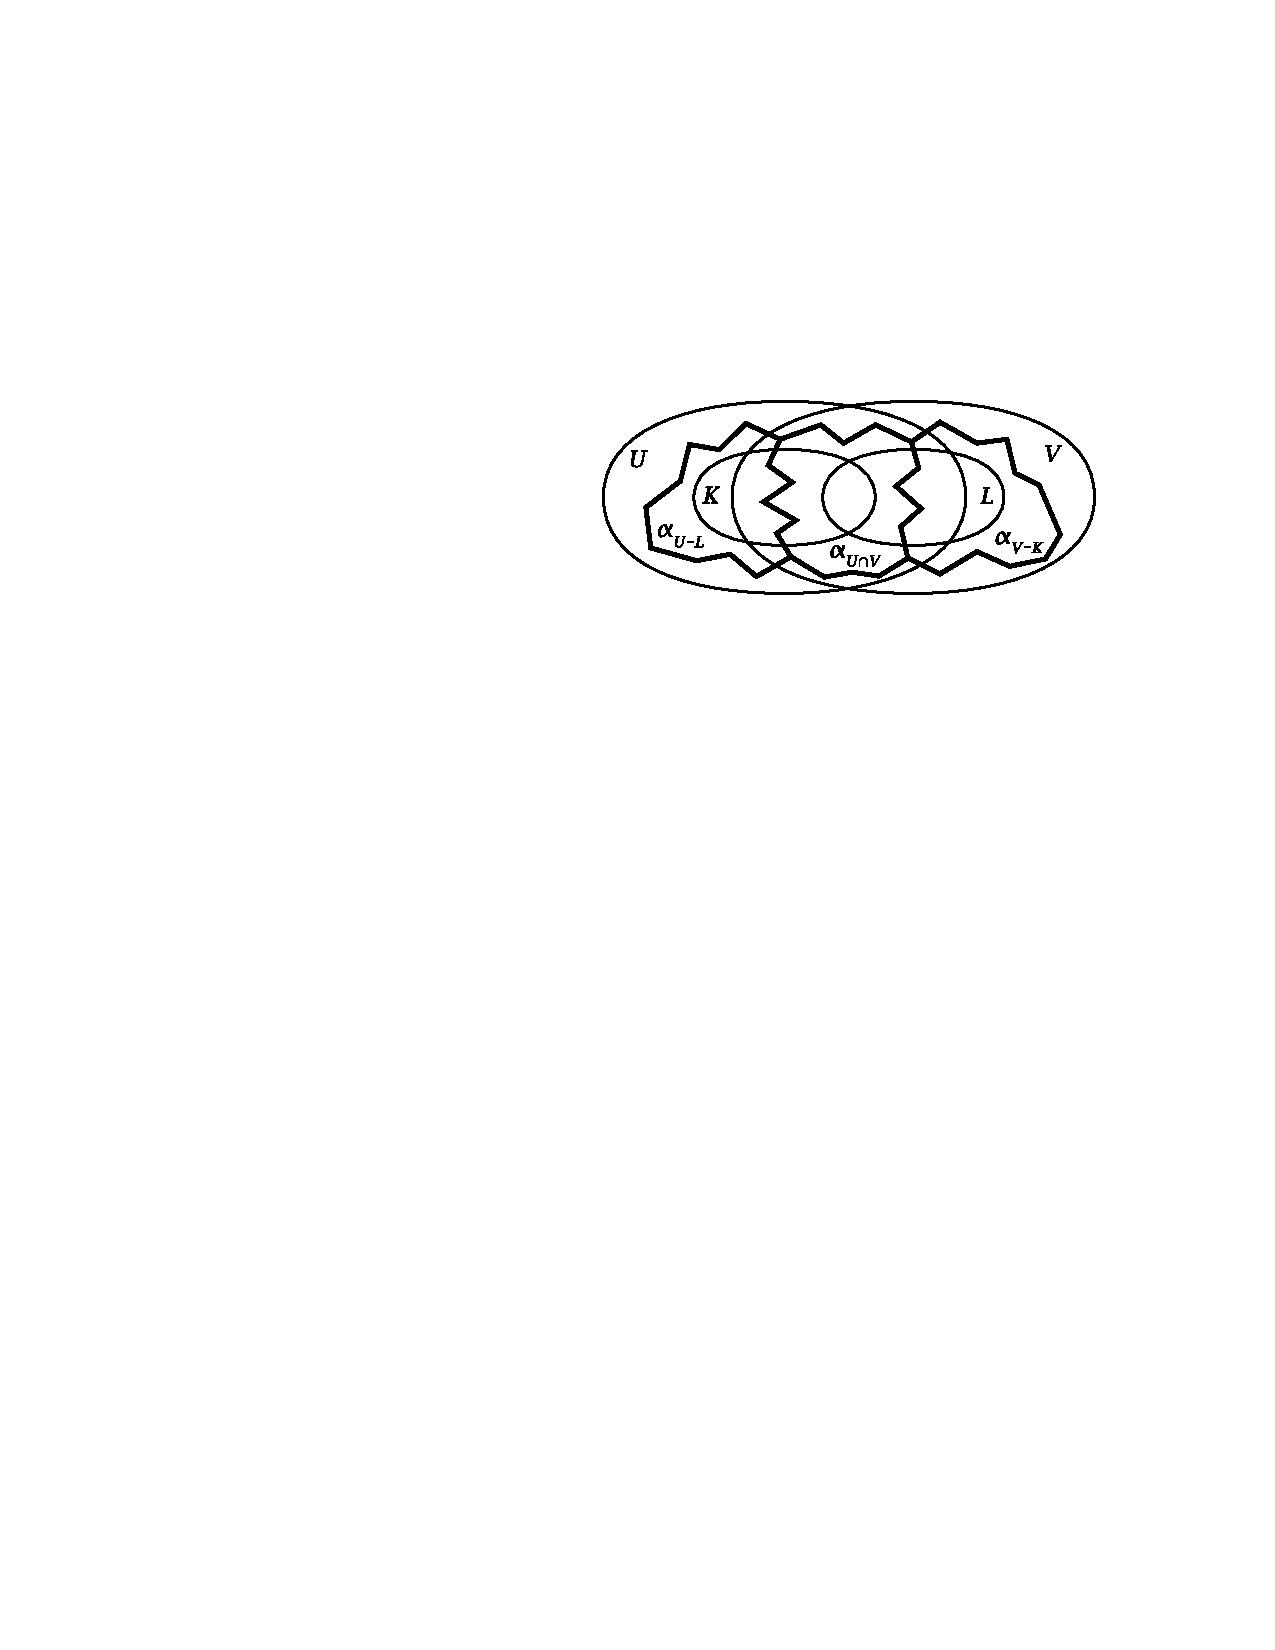
\includegraphics{Duality}
\end{figure}
In the square $(*) $ let $\varphi$ be a cocycle representing an element of $H^k(M|K\cup L)$. Under $\delta$ this maps to the cohomology class of $\delta\varphi_A$. Continuing on to $H_{n-k-1}(U\cap V)$ we obtain $\alpha_{U\cap V}\cap\delta\varphi_A$, which is in the same homology class as $\partial\alpha_{U\cap V}\cap\varphi_A$ since
\[\partial(\alpha_{U\cap V}\cap\varphi_A)=(-1)^k(\partial\alpha_{U\cap V}\cap\varphi_A-\alpha_{U\cap V}\cap\delta\varphi_A)\]
and $\alpha_{U\cap V}\cap\varphi_A$ is a chain in $U\cap V$.\par
Going around the square $(*)$ the other way, $\varphi$ maps first to $\alpha\cap\varphi$. To apply the Mayer-Vietoris boundary map $\partial$ to this, we first write $\alpha\cap\varphi$ as a sum of a chain in $U$ and a chain in $V$:
\[\alpha\cap\varphi=(\alpha_{U-L}\cap\varphi)+(\alpha_{U\cap V}\cap\varphi+\alpha_{V-K}\cap\varphi)\]
Then we take the boundary of the first of these two chains, obtaining the homology class $[\partial(\alpha_{U-L}\cap\varphi)]\in H_{n-k-1}(U\cap V)$. To compare this with $[\partial\alpha_{U\cap V}\cap\varphi_A]$, we have
\begin{align*}
\partial(\alpha_{U-L}\cap\varphi)&\stackrel{1}{=}(-1)^k\partial\alpha_{U-L}\cap\varphi\stackrel{2}{=}(-1)^k\partial\alpha_{U-L}\cap\varphi_A\\
&\stackrel{3}{=}(-1)^{k+1}\partial\alpha_{U\cap V}\cap\varphi_A
\end{align*}
where $\stackrel{1}{=}$ comes from $\delta\varphi=0$, $\stackrel{2}{=}$ from $\partial\alpha_{U-L}\cap\varphi_B=0$ since $\varphi_B$ is zero on chains in $B=M-L$. And $\stackrel{3}{=}$ comes from the fact that $\partial(\alpha_{U-L}+\alpha_{U\cap V})\cap\varphi_A=0$ since $\partial(\alpha_{U-L}+\alpha_{U\cap V})$ is a chain in $U-K$ by the earlier observation that $\alpha_{U-L}+\alpha_{U\cap V}$ represents $\mu_K$, and $\varphi_A$ vanishes on chains in $A=M-K$.\par
Thus the square $(*)$ commutes up to a sign depending only on $k$.
\end{proof}
\begin{proof}[\textbf{Proof of Poincar\'e Duality}]
There are two inductive steps, finite and infinite:
\begin{itemize}
\item[$(A)$]If $M$ is the union of open sets $U$ and $V$ and if $D_U$, $D_V$, and $D_{U\cap V}$ are isomorphisms, then so is $D_M$. Via the five-lemma, this is immediate from the preceding lemma. (Even though the commutativity is up to a sign, we can still use the five lemma.)
\item[$(B)$]If $M$ is the union of a sequence of open sets $U_1\sub U_2\sub\cdots$ and each duality map $D_{U_i}:H^k_c(U_i)\to H_{n-k}(U_i)$ is an isomorphism, then so is $D_M$. To show this we notice first that by excision, $H^k_c(U_i)$ can be regarded as the limit of the groups $H^k(M|K)$ as $K$ ranges over compact subsets of $U_i$. Then there are natural maps $H^k_c(U_i)\to H^k_c(U_{i+1})$ since the second of these groups is a limit over a larger collection of $K$'s. Thus we can form $\rlim H^k_c(U_i)$ which is obviously isomorphic to $H^k_c(M)$ since the compact sets in $M$ are just the compact sets in all the $U_i$'s. By Proposition~\ref{homology limit}, $H_{n-k}(M)\cong\rlim H_{n-k}(U_i)$. The map $D_M$ is thus the limit of the isomorphisms $D_{U_i}$, hence is an isomorphism.
\end{itemize}
Now after all these preliminaries we can prove the theorem in three easy steps:
\begin{itemize}
\item[$(1)$]The case $M=\R^n$ can be proved by regarding $\R^n$ as the interior of $\Delta^n$, and then the map $D_M$ can be identified with the map $H^k(\Delta^n,\partial\Delta^n)\to H_{n-k}(\Delta^n)$ given by cap product with a unit times the generator $[\Delta^n]\in H_n(\Delta^n,\partial\Delta^n)$ defined by the identity map of $\Delta^n$, which is a relative cycle. The only nontrivial value of $k$ is $k=n$, when the cap product map is an isomorphism since a generator of $H^n(\Delta^n,\partial\Delta^n)\cong\Hom(H_n(\Delta^n,\partial\Delta^n),R)$ is represented by a cocycle $\varphi$ taking the value $1$ on $\Delta^n$, so by the definition of cap product, $\Delta^n\cap\varphi$ is the last vertex of $\Delta^n$, representing a generator of $H_0(\Delta^n)$.
\item[$(2)$]More generally, $D_M$ is an isomorphism for $M$ an arbitrary open set in $\R^n$. To see this, first write $M$ as a countable union of nonempty bounded convex open sets $U_i$, for example open balls, and let $V_i=\bigcup_{j<i}U_j$. Both $V_i$ and $U_i\cap V_i$ are unions of $i-1$ bounded convex open sets, so by induction on the number of such sets in a cover we may assume that $D_{V_i}$ and $D_{U_i\cap V_i}$ are isomorphisms. By $(1)$, $D_{U_i}$ is an isomorphism since $U_i$ is homeomorphic to $\R^n$. Hence $D_{U_i\cup V_i}$ is an isomorphism by $(A)$. Since $M$ is the increasing union of the $V_i$'s and each $D_{V_i}$ is an isomorphism, so is $D_M$ by $(B)$.
\item[$(3)$]If $M$ is a finite or countably infinite union of open sets $U_i$ homeomorphic to $\R^n$, the theorem now follows by the argument in $(2)$, with each appearance of the words bounded convex open set replaced by open set in $\R^n$. Thus the proof is finished for closed manifolds, as well as for all the noncompact manifolds one ever encounters in actual practice.
\end{itemize}
To handle a completely general noncompact manifold $M$ we use a Zorn's Lemma
argument. Consider the collection of open sets $U\sub M$ for which the duality maps $D_U$ are isomorphisms. This collection is partially ordered by inclusion, and the union of every totally ordered subcollection is again in the collection by the argument in $(B)$, which did not really use the hypothesis that the collection $\{U_i\}$ was indexed by the positive integers. Zorn's Lemma then implies that there exists a maximal open set $U$ for which the theorem holds. If $U\neq M$, choose a point $x\in M-U$ and an open neighborhood $V$ of $x$ homeomorphic to $\R^n$. The theorem holds for $V$ and $U\cap V$ by $(1)$ and $(2)$, and it holds for $U$ by assumption, so by $(A)$ it holds for $U\cup V$, contradicting the maximality of $U$.
\end{proof}
\begin{corollary}
A closed manifold of odd dimension has Euler characteristic zero.
\end{corollary}
\begin{proof}
Let $M$ be a closed $n$-manifold. If $M$ is orientable, we have $\rank H_i(M;\Z)=\rank H^{n-i}(M;\Z)$, which equals $\rank H_{n-i}(M;\Z)$ by the universal coefficient theorem. Thus if $n$ is odd, all the terms of $\sum_i(-1)^i\rank H_i(M;\Z)$ cancel in pairs.\par
If $M$ is not orientable we apply the same argument using $\Z/2\Z$ coefficients, with $\rank H_i(M;\Z)$ replaced by $\dim H_i(M;\Z/2\Z)$, the dimension as a vector space over $\Z/2\Z$. It remains to check that the alternating sum $\sum_i(-1)^i\dim H_i(M;\Z/2\Z)$ equals the Euler characteristic $\sum_i(-1)^i\rank H_i(M;\Z)$. We can do this by using
the universal coefficient theorem for cohomology. Each $\Z$ summand of $H_i(M;\Z)$ gives a $\Z/2\Z$ summand of $H^i(M;\Z/2\Z)$. Each $\Z/m\Z$ summand of $H_i(M;\Z)$ with $m$ even gives $\Z/2\Z$ summands of $H^i(M;\Z/2\Z)$ and $H_{i+1}(M,\Z/2\Z)$, whose contributions to $\sum_i(-1)^i\dim H_i(M;\Z/2\Z)$ cancel. And $\Z/m\Z$ summands of $H_i(M;\Z)$ with $m$ odd contribute nothing to $H^*(M;\Z/2\Z)$.
\end{proof}
\subsection{Connection with Cup Product}
Cup and cap product are related by the formula
\begin{align}
\psi(\alpha\cap\varphi)=(\varphi\cup\psi)(\alpha)\tag{$\ast$}
\end{align}
for $\alpha\in C_{k+\ell}(X;R)$, $\varphi\in C^k(X;R)$, and $\psi\in C^\ell(X;R)$. This holds since for a singular $(k+\ell)$ simplex $\sigma:\Delta^{k+\ell}\to X$ we have
\begin{align*}
\psi(\sigma\cap\varphi)&=\psi(\varphi(\sigma|[v_0,\cdots,v_k])\,\sigma|[v_k,\cdots,v_{k+\ell}])\\
&=\varphi(\sigma|[v_0,\cdots,v_k])\,\psi(\sigma|[v_k,\cdots,v_{k+\ell}])\\
&=(\varphi\cup\psi)(\sigma)
\end{align*}
The formula $(*)$ says that the map $\varphi\cup:C^\ell(X;R)\to C^{k+\ell}(X;R)$ is equal to the map $\Hom_R(C^\ell(X;R),R)\to\Hom_R(C^{k+\ell}(X;R),R)$ dual to $\cap\varphi$. Passing to homology and cohomology, we obtain the commutative diagram
\[\begin{tikzcd}
H^\ell(X;R)\ar[r,"h"]\ar[d,"\varphi\cup"]&\Hom_R(H_\ell(X;R),R)\\
H^{k+\ell}(X;R)\ar[r,"h"]&\Hom_R(H_{k+\ell}(X;R),R)\ar[u,"(\cap\varphi)^*"]
\end{tikzcd}\]
When the maps $h$ are isomorphisms, for example when $R$ is a field or when $R=\Z$ and the homology groups of $X$ are free, then the map $\varphi\cup$ is the dual of $\cap\varphi$. Thus in these cases cup and cap product determine each other, at least if one assumes finite generation so that cohomology determines homology as well as vice versa. However, there are examples where cap and cup products are not equivalent when $R=\Z$ and there is torsion in homology.\par
By means of the formula $(*)$, Poincar\'e duality has nontrivial implications for the cup product structure of manifolds. For a closed $R$-orientable $n$ manifold $M$, consider the cup product pairing
\[H^k(M;R)\times H^{n-k}(M;R)\to R,\quad (\varphi,\psi)\mapsto(\varphi\cup\psi)[M]\]
Such a bilinear pairing $A\times B\to R$ is said to be \textbf{nonsingular} if the maps $A\to\Hom_R(B,R)$ and $B\to\Hom_R(A,R)$, obtained by viewing the pairing as a function of each variable separately, are both isomorphisms.
\begin{proposition}
The cup product pairing is nonsingular for closed $R$-orientable manifolds when $R$ is a field, or when $R=\Z$ and torsion in $H^*(M;\Z)$ is factored out.
\end{proposition}
\begin{proof}
Consider the composition
\[\begin{tikzcd}
H^{n-k}(M;R)\ar[r,"h"]&\Hom_R(H_{n-k}(M;R),R)\ar[r,"D^*"]&\Hom(H^{k}(M;R),R)
\end{tikzcd}\]
where $h$ is the map appearing in the universal coefficient theorem, induced by evaluation of cochains on chains, and $D^*$ is the Hom dual of the Poincar\'e duality map $D:H^k\to H_{n-k}$. The composition $D^*h$ sends $\psi\in H^{n-k}(M;R)$ to the homomorphism $\varphi\mapsto\psi([M]\cap\varphi)=(\varphi\cup\psi)[M]$. For field coefficients or for integer coefficients with torsion factored out, $h$ is an isomorphism. Nonsingularity of the pairing in one of its variables is then equivalent to $D$ being an isomorphism. Nonsingularity in the other variable follows by commutativity of cup product.
\end{proof}
\begin{corollary}
If $M$ is a closed connected orientable $n$-manifold, then an element $\alpha\in H^k(M;\Z)$ generates an infinite cyclic summand of $H^k(M;\Z)$ iff there exists an element $\beta\in H_{n-k}(M;\Z)$ such that $\alpha\cup\beta$ is a generator of $H_n(M;\Z)=\Z$. With coefficients in a field this holds for any $\alpha\neq0$.
\end{corollary}
\begin{proof}
For $\alpha$ to generate a $\Z$ summand of $H^k(M;\Z)$ is equivalent to the existence of a homomorphism $\varphi:H^k(M;\Z)\to\Z$ with $\varphi(\alpha)=\pm1$. By the nonsingularity of the cup product pairing, $\varphi$ is realized by taking cup product with an element $\beta\in H_{n-k}(M;\Z)$ and evaluating on $[M]$, so having a $\beta$ with $\alpha\cup\beta$ generating $H_n(M;\Z)$ is equivalent to having $\varphi$ with $\varphi(\alpha)=\pm1$. The case of field coefficients is similar but easier.
\end{proof}
\subsection{Other Forms of Duality}
Generalizing the definition of a manifold, an $n$-manifold with boundary is a
Hausdorff space $M$ in which each point has an open neighborhood homeomorphic
either to $\R^n$ or to the half-space $\R^n_+$.\par
If $M$ is a manifold with boundary, then a \textbf{collar} neighborhood of $\partial M$ in $M$ is an open neighborhood homeomorphic to $\partial M\times[0,1)$ by a homeomorphism taking $\partial M$ to $\partial M\times\{0\}$.
\begin{proposition}
If $M$ is a $n$-manifold with boundary, then $\partial M$ has a collar neighborhood.
\end{proposition}
\begin{proof}
Let $M'$ be $M$ with an external collar attached, the quotient of the disjoint union of $M$ and $\partial M\times[-1,0]$ in which $x\in\partial M$ is identified with $(x,0)\in\partial M\times[-1,0]$. Observe that $M'$ is also a $n$-manifold with its boundary homeomorphic to $\partial M\times\{-1\}$. It will suffice to construct a homeomorphism $h:M\to M'$ since $\partial M'$ has a collar neighborhood $\partial M\times[-1,0)$.\par
Begin with a partition of unity $\{\varphi_i\}$ on $\partial M$ such that $\supp\varphi_i$ is contained in a coordinate open set $U_i$ of $\partial M$ together with a homeomorphism $\phi_i $ from $U_i\times[0,1)$ onto an open subset $V_i$ of $M$. Let \[\psi_k=\sum_{i=1}^k\varphi_i,\quad M_k:=M\cup\{(x,t)\in\partial M\times[-1,0]:-\psi_k(x)\leq t\leq 0\}\]
By definition $\psi_0=0$ and $M_0=M$. We construct a homeomorphism $h_k:M_{k-1}\to M_k$ as follows.
\begin{itemize}
\item First consider the spaces $U_i\times[-1,0]$, define
\[Z_k:=\{(x,t)\in U_k\times[-1,1]:-\psi_{k-1}\leq t\leq1\};\quad Z'_k=\{(x,t)\in U_k\times[-1,1]:-\psi_{k}\leq t\leq 1\}\]
Let $\alpha_k:Z_k\to Z_k'$ be the homeomorphism which linearly stretches the segment $[-\psi_{k-1}(x),1]$ homeomorphically onto the segment $[-\psi_k(x),1]$, for each $x$.
\item let $\beta_k:Z'_k\to M_k$ be the embeddings given by
\[\beta_k(x,t)=\begin{cases}
\phi_k(x,t),&t\geq 0\\
(x,t),&t\leq 0
\end{cases}\]
\item We define homeomorphisms $h_k:M_{k-1}\to M_k$ as follows:
\[h_k(z)=\begin{cases}
z,&z\in M-\phi_k(U_k\times[0,1))\\
(x,t),&z=(x,t),x\notin U_k\\
\beta_k\circ\alpha_k(x,t),&z\in\phi_k(U_k\times[0,1))\text{ with }z=\phi_k(x,t)\\
\beta_k\circ\alpha_k(x,t),&x\in U_k, t\leq 0
\end{cases}\]
So $h_k$ is identity outside $U_k\times[-1,1]$, and for $x\in U_k$ it stretches the segment $\{x\}\times[-1,\psi_{k-1}(x)]$ linearly onto $\{x\}\times[-1,\psi_k(x)]$.
\end{itemize} 
The composition of all the $h_k$'s then gives a map $h:M\to M'$. First of all note that on the complement of $V=\bigcup_i\phi_i(U_i\times[0,1))$, $h$ is identity. On $V$ itself, $h$ makes sense, since given any point $x\in\partial M$, there are only finitely many $i$ for which $x\in U_i$ and $h_k(x,t)=(x,t)$ if $x\notin U_k$. Indeed in a neighbourhood of $x$, all $h_k$ are identity except those $k$ for which $\varphi_k(x)\neq 0$. For this reason, $h$ is also a proper mapping. Since $\sum_k\varphi_k(x)=1$, it follows that $h$ is surjective. Since each $h_k$ is an embedding $h$ is injective. Therefore $h$ is a homeomorphism.
\end{proof}
A compact manifold $M$ with boundary is defined to be $R$-orientable if $M-\partial M$ is $R$-orientable as a manifold without boundary. If $\partial M\times[0,1)$ is a collar neighborhood of $\partial M$ in $M$ then $H_i(M,\partial M;R)$ is naturally isomorphic to $H_i(M-\partial M,\partial M\times(0,\eps);R)$, so when $M$ is $R$-orientable, Lemma~\ref{orientation lem} gives a relative fundamental class $[M]$ in $H_n(M,\partial M;R)$ restricting to a given orientation at each point of $M-\partial M$.\par
It will not be difficult to deduce the following generalization of Poincar\'e duality to manifolds with boundary from the version we have already proved for noncompact manifolds:
\begin{theorem}
Suppose $M$ is a compact $R$-orientable $n$-manifold whose boundary $\partial M$ is decomposed as the union of two compact $(n-1)$-dimensional manifolds $A$ and $B$ with a common boundary $\partial A=\partial B=A\cap B$. Then cap product with a fundamental class $[M]\in H_n(M,\partial M;R)$ gives isomorphisms $D_M:H_k(M,A;R)\to H_{n-k}(M,B;R)$ for all $k$.
\end{theorem}
\begin{proof}
The cap product map $D_M:H^k(M,A;R)\to H_{n-k}(M,B;R)$ is defined since the
existence of collar neighborhoods of $A\cap B$ in $A$ and $B$ and $\partial M$ in $M$ implies that $A$ and $B$ are deformation retracts of open neighborhoods $U$ and $V$ in $M$ such that $U\cup V$ deformation retracts onto $A\cup B=\partial M$ and $U\cap V$ deformation retracts onto $A\cap B$.\par
The case $B=\emp$ is proved by applying Theorem~\ref{Poincare duality} to $M-\partial M$. Via a collar neighborhood of $\partial M$ we see that $H^k(M,\partial M;R)\cong H^k_c(M-\partial M;R)$, and there are obvious isomorphisms $H_{n-k}(M;R)\cong H_{n-k}(M-\partial M;R)$.\par
The general case reduces to the case $B=\emp$ by applying the five-lemma to \[\begin{tikzcd}
\cdots\ar[r]&H^k(M,\partial M)\ar[dd,"{[M]\cap}"]\ar[r]&H^k(M,A)\ar[dd,"{[M]\cap}"]\ar[r]&H^k(\partial M,A)\ar[d,"\cong"]\ar[r]&H^{k+1}(M,\partial M)\ar[dd,"{[M]\cap}"]\ar[r]&\cdots\\
&&&H^k(B,\partial B)\ar[d,"{[B]\cap}"]&&\\
\cdots\ar[r]&H_{n-k}(M)\ar[r]&H_{n-k}(M,B)\ar[r]&H_{n-k}(B)\ar[r]&H_{n-k-1}(M)\ar[r]&\cdots
\end{tikzcd}\]
For commutativity of the middle square one needs to check that the boundary map $H_n(M,\partial M)\to H_{n-1}(\partial M)$ sends a fundamental class for $(M,\partial M)$ to a fundamental class for $\partial M$. We identify $(0,1)\times\partial M$ with its image in $M$, and let
\[K=M-[0,1)\times\partial M\sub M-\partial M.\]
Consider the following diagram for $x\in(0,1)\times\partial M$:
\[\begin{tikzcd}
H_{n-1}(\partial M)\ar[r,"\cong"]&H_{n-1}(\partial M\cup K,K)&H_{n-1}(\partial I\times\partial M,\{1\}\times\partial M)\ar[l,swap,"\cong"]\\
H_n(M,\partial M)\ar[u,"\partial"]\ar[rd]\ar[r]&H_n(M,\partial M\cup K)\ar[u,"\partial","\cong"']\ar[d]&H_{n}(I\times\partial M,\partial I\times\partial M)\ar[l,swap,"\cong"]\ar[u,"\partial","\cong"']\ar[d]\\
&H_n(M,M-x)&H_{n}(I\times\partial M,I\times\partial M-x)\ar[l,swap,"\cong"]
\end{tikzcd}\]
This shows $[M]$ restricts to a generator of $H_{n}(I\times\partial M|x)$, hence a fundamental class in $H_n(I\times\partial M,\partial I\times\partial M)$. The upper part shows that this fundamental class corresponds to a fundamental class in $H_{n-1}(\partial M)$, since fundamental classes are characterized by the fact that they are generators.
\end{proof}
Here is another kind of duality which generalizes the calculation of the local homology groups $H_i(M,M-\{x\};\Z)$:
\begin{theorem}\label{loc contract dual}
If $K$ is a compact, locally contractible subspace of a closed orientable $n$-manifold $M$, then $H_i(M,M-K;\Z)\cong H^{n-i}(K;\Z)$ for all $i$.
\end{theorem}
\begin{proof}
Let $U$ be an open neighborhood of $K$ in $M$. Consider the following diagram whose rows are long exact sequences of pairs and isomorphisms come from excision:
\[\begin{tikzcd}[column sep=small]
\cdots\ar[r]&H_i(M-K)\ar[r]&H_i(M)\ar[r]&H_i(M,M-K)\ar[r]&H_{i-1}(M-K)\ar[r]&\cdots\\
&H^{n-i}(M-K,U-K)\ar[u]&&H_i(U,U-K)\ar[u,"\cong"]&H^{n-i+1}(M-K,U-K)\ar[u]&\\
\cdots\ar[r]&H^{n-i}(M,U)\ar[u,"\cong"]\ar[r]&H^{n-i}(M)\ar[uu]\ar[r]&H^{n-i}(U)\ar[r]\ar[u]&H^{n-i+1}(M,U)\ar[r]\ar[u,"\cong"]&\cdots
\end{tikzcd}\]
The second vertical map is the Poincar\'e duality isomorphism given by cap products with a fundamental class $[M]$. This class can be represented by a cycle which is the sum of a chain in $M-K$ and a chain in $U$ representing elements of $H_n(M-K,U-K)$ and $H_n(U,U-K)$ respectively, and the first and third vertical maps are given by relative cap products with these classes. It is not hard to check that the diagram commutes up to sign, where for the square involving boundary and coboundary maps one uses the formula for the boundary of a cap product.\par
Passing to the direct limit over decreasing $U\sups K$, the first vertical arrow become the Poincar\'e duality isomorphism $H_i(M-K)\cong H^{n-i}_c(M-K)$. The five-lemma then gives an isomorphism $H_i(M,M-K)\cong\rlim H^{n-i}(U)$. We will show that the natural
map from this limit to $H^{n-i}(K)$ is an isomorphism. This is easy when $K$ has a neighborhood that is a mapping cylinder of some map $X\to K$, since in this case we can compute the direct limit using neighborhoods $U$ which are segments of the mapping cylinder that deformation retract to $K$.\par
For the general case, $M$ can be embedded in some $\R^k$ as a retract of a neighborhood $N$ in $\R^k$, and $K$ is a retract of a neighborhood in $\R^k$
and hence, by restriction, of a neighborhood $W$ in $M$. We can compute $\rlim H^{n-i}(U)$ using just neighborhoods $U$ in $W$, so these also retract to $K$ and hence the map $\lim H_{n-i}(U)\to H_{n-i}(K)$ is surjective. To show that it is injective, note first that the
retraction $U\to K$ is homotopic to the identity $U\to U$ through maps $U\to\R^k$, via the standard linear homotopy. Choosing a smaller $U$ if necessary, wemay assume this homotopy is through maps $U\to N$ since $K$ is stationary during the homotopy. Applying the retraction $N\to M$ gives a homotopy through maps $U\to M$ fixed on $K$. Restricting to sufficiently small $V\sub U$, we then obtain a homotopy in $U$ from the inclusion map $V\to U$ to the retraction $V\to K$. Thus the map $H_{n-i}(U)\to H_{n-i}(V)$ factors as $H_{n-i}(U)\to H_{n-i}(K)\to H_{n-i}(V)$ where the first map is induced by inclusion and the second by the retraction. This implies that the kernel of $\rlim H_{n-i}(U)\to H_{n-i}(K)$ is trivial.
\end{proof}
From this theorem we can easily deduce \textbf{Alexander duality}:
\begin{corollary}
If $K$ is a compact, locally contractible, nonempty, proper subspace of $S^n$, then $\widetilde{H}_i(S^n-K;\Z)\cong\widetilde{H}^{n-i-1}(K;\Z)$ for all $i$.
\end{corollary}
\begin{proof}
The long exact sequence of reduced homology for the pair $(S^n,S^n-K)$ gives
isomorphisms $\widetilde{H}^i(S^n-K;\Z)\cong H_{i+1}(S^n,S^n-K;\Z)$ for most values of $i$. The exception is when $i=n-1$ and we have only a short exact sequence
\[\begin{tikzcd}
0\ar[r]&\widetilde{H}_n(S^n;\Z)\ar[r]&H_n(S^n,S^n-K;\Z)\ar[r]&\widetilde{H}_{n-1}(S^n-K;\Z)\ar[r]&0
\end{tikzcd}\]
where the initial $0$ is $\widetilde{H}_n(S^n-K;\Z)$ which is zero since the components of $S^n-K$ are noncompact $n$-manifolds. This short exact sequence splits since we can map it to the corresponding sequence with $K$ replaced by a point in $K$. Thus $\widetilde{H}_{n-1}(S^n-K;\Z)$ is $H_n(S^n,S^n-K;\Z)$ with a $\Z$ summand canceled, just as $\widetilde{H}^0(K;\Z)$ is $H^0(K;\Z)$ with a $\Z$ summand canceled.
\end{proof}
\begin{corollary}
If $X\sub\R^n$ is compact and locally contractible then $H_i(X;\Z)$ is $0$ for $i\geq n$ and torsion-free for $i=n-1$ and $n-2$.
\end{corollary}
For example, a closed nonorientable $n$-manifold $M$ cannot be embedded as a subspace of $\R^{n+1}$ since $H_{n-1}(M;\Z)$ contains a $\Z/2\Z$ subgroup, by Corollary~\ref{homology n-mani n-1}. Thus the Klein bottle cannot be embedded in $\R^3$. 
\begin{proof}
Viewing $X$ as a subspace of the one-point compactification $S^n$, Alexander
duality gives isomorphisms $\widetilde{H}^i(X;\Z)\cong\widetilde{H}^{n-i-1}(S^n-X;\Z)$. The latter group is zero for $i\geq n$ and torsionfree for $i=n-1$, so the result follows from the universal coefficient theorem since $X$ has finitely generated homology groups.
\end{proof}
There is a way of extending Alexander duality and the duality in Theorem~\ref{loc contract dual} to compact sets $K$ that are not locally contractible, by replacing the singular cohomology of $K$ with another kind of cohomology called \textbf{\v{C}ech cohomology}. This is defined in
the following way. To each open cover $\mathcal{U}=\{U_\alpha\}$ of a given space $X$ we can associate a simplicial complex $N(\mathcal{U})$ called the \textbf{nerve} of $\mathcal{U}$. This has a vertex $v_\alpha$ for each $U_\alpha$, and a set of $k+1$ vertices spans a $k$-simplex whenever the $k+1$ corresponding $U_\alpha$'s have nonempty intersection. When another cover $\mathcal{V}=\{V_\beta\}$ is a refinement of $\mathcal{U}$, so each $V_\beta$ is contained in some $U_\alpha$, then these inclusions induce a simplicial map $N(\mathcal{V})\to N(\mathcal{U})$ that is well-defined up to homotopy. We can then form the direct limit $\rlim H^i(N(\mathcal{U});G)$ with respect to finer and finer open covers $\mathcal{U}$. This limit group is by definition the \v{C}ech cohomology group $\check{H}^i(X;G)$.
\subsection{Exercise}
\begin{exercise}
Show that there exist nonorientable $1$-dimensional manifolds if the Hausdorff  condition is dropped from the definition of a manifold.
\end{exercise}
\begin{proof}
Let $X$ be the subset $([-1,1]\times\{0\})\cup([-1,1]\times\{1\})\sub\R^2$. Define an equivalence relation on $X$ by declaring $(0,0)\sim(0,1)$. Show that the quotient space $X/\sim$ is locally Euclidean and second countable, but not Hausdorff. Calculating the homology we find $H^1(X/\sim)=0$, so $X/\sim$ is not oritentable.
\end{proof}
\begin{exercise}
Show that deleting a point from a manifold of dimension greater than $1$ does not affect orientability of the manifold.
\end{exercise}
\begin{proof}
By excision we can show an orientation class in $M-x$ extends to that in $M$.
\end{proof}
\begin{exercise}
Given a covering space action of a group $G$ on an orientable manifold $M$ by orientation-preserving homeomorphisms, show that $M/G$ is also orientable.
\end{exercise}
\begin{exercise}
Show that $M\times N$ is orientable iff $M$ and $N$ are both orientable.
\end{exercise}
\begin{proof}
If $M$ is orientable, then every open set in $M$ is also orientable.\par
For $M$ and $\R^k$, we have $\widetilde{M\times\R^k}\approx\widetilde{M}\times\R^k$, which is done by $(\mu_x,y)\mapsto\mu_{(x,y)}$. Hence if $M$ is not orientable, then $M\times\R^k$ is not orientable for any $k$.\par
Now for $M\times N$, choose a neighborhood $M\times B^k$. If $M$ is not orientable, then this is not orientable, hence $M\times N$ is not orientable.\par
If $M$, $N$ are orientable, then $M\times B^k$ are orientable for any $B^k$ open in $N$. Since we can choose a orientation class $\mu_N$ restricting to generator in each ball $B^k$, we see $M\times N$ is orientable.
\end{proof}
\begin{exercise}
Given two connected $n$-manifolds $M_1$ and $M_2$,
\begin{itemize}
\item[$(a)$]Show that if $M_1$ and $M_2$ are closed then there are isomorphisms $H_i(M_1\#M_2;\Z)\cong H_i(M_1;\Z)\oplus H_i(M_2;\Z)$ for $0<i<n$, with one exception: If both $M_1$ and $M_2$ are nonorientable, then $H_{n-1}(M_1\#M_2;\Z)$ is obtained from $H_{n-1}(M_1\#M_2;\Z)\cong H_{n-1}(M_1;\Z)\oplus H_i(M_2;\Z)$ by replacing one of the two $\Z/2\Z$ summands by a $\Z$ summand.
\item[$(b)$]Show that $\chi(M_1\#M_2)=\chi(M_1)+\chi(M_2)-\chi(S^n)$ if $M_1$ and $M_2$ are closed.
\end{itemize}
\end{exercise}